\documentclass{beamer}

\usepackage{graphics}
\usepackage{graphicx}
\usepackage{amsmath,amssymb,amsthm}
\usepackage{cancel}
%\usepackage{subeqnarray}
%\usepackage{easybmat}
%\usepackage{subfigure}



%\usepackage{HA-prosper}
%\usepackage[dvips,letterpaper]{geometry}

\def\M{\mathcal{M}}
\def\R{\mathcal{R}}
\def\D{\mathcal{D}}
\def\C{\mathcal{C}}
\def\I{\mathcal{I}}
\def\IC{\mathbb{C}}
\def\IN{\mathbb{N}}
\def\IR{\mathbb{R}}
\def\IK{\mathbb{K}}
\def\II{\mathbb{I}}
\def\IZ{\mathbb{Z}}
\def\Rzero{\mathcal{R}_0}
\def\diag{\textrm{diag}}
\def\tr{\ensuremath{\mathsf{tr}}}
\def\det{\ensuremath{\mathsf{det}}}
\def\Span{\ensuremath{\mathsf{span}}}
\def\sgn{\textrm{sgn}}
\def\sign{\textrm{sign}}
\def\imply{$\Rightarrow$}
\def\dbint{\int\!\!\!\int}
\def\dbintb{\mathop{\int\!\!\!\!\int}}
\def\tpint{\int\!\!\!\int\!\!\!\int}
\def\Proba#1{\mathcal{P}\left(#1\right)}
\def\Surv{\mathcal{S}}

\def\R{\mathcal{R}}
\def\D{\mathcal{D}}
\def\C{\mathcal{C}}
\def\IC{\mathbb{C}}
\def\IN{\mathbb{N}}
\def\IR{\mathbb{R}}
\def\Rzero{\mathcal{R}_0}
\def\diag{\textrm{diag}}
\def\tr{\textrm{tr}}
\def\det{\textrm{det}}
\def\sgn{\textrm{sgn}}
\def\imply{$\Rightarrow$}
\def\dbint{\int\!\!\!\int}
\def\dbintb{\mathop{\int\!\!\!\!\int}}
\def\tpint{\int\!\!\!\int\!\!\!\int}
\def\nbOne{{\mathchoice {\rm 1\mskip-4mu l} {\rm 1\mskip-4mu l}
{\rm 1\mskip-4.5mu l} {\rm 1\mskip-5mu l}}}

\newtheorem{proposition}{Proposition}

\setbeamertemplate{theorems}[numbered]
\setbeamertemplate{navigation symbols}{}
\setbeamertemplate{footline}
{%
\quad\insertsection\hfill p. \insertpagenumber\quad\mbox{}\vskip2pt
}

\AtBeginSection[]
{
\begin{frame}<beamer>
\frametitle{Outline}
%\tableofcontents[currentsection,hideothersubsections]
\tableofcontents[sectionstyle=show/hide,subsectionstyle=show/show/hide]
\end{frame}
}

\AtBeginSection[]
{
\begin{frame}<beamer>
\frametitle{Outline}
\tableofcontents[currentsection,hideothersubsections]
%\tableofcontents[sectionstyle=show/hide,subsectionstyle=show/show/hide]
\end{frame}
}

% \AtBeginSection[]
% {
% }

\AtBeginSubsection[]
{
\begin{frame}<beamer>
\tableofcontents[sectionstyle=show/hide,subsectionstyle=show/shaded/hide]
\end{frame}
}

% \AtBeginSubsection[]
% {
% }

\title{Summary of topics relevant for the final}
\date{}


\begin{document}
\frame{\titlepage}

\frame{\frametitle{Mathematical techniques}
\tableofcontents[part=1,hideallsubsections]
}


%\maketitle
%%%%%%%%%%%%%%
%%%%%%%%%%%%%%
%%%%%%%%%%%%%%
%%%%%%%%%%%%%%
%%%%%%%%%%%%%%
%%%%%%%%%%%%%%
%%%%%%%%%%%%%%
%%%%%%%%%%%%%%
\part{Mathematical techniques}


%%%%%%%%%%%%%%
%%%%%%%%%%%%%%
%%%%%%%%%%%%%%
%%%%%%%%%%%%%%
\section{Regression}
\frame{\frametitle{Regression}
See Dr. Berry's notes.
}

%%%%%%%%%%%%%%
%%%%%%%%%%%%%%
%%%%%%%%%%%%%%
%%%%%%%%%%%%%%
\section{Discrete time systems}

\frame{\frametitle{Discrete-time systems}
So far, we have seen continuous-time models, where $t\in\IR_+$. Another way to model natural phenomena is by using a discrete-time formalism, that is, to consider equations of the form
\[
x_{t+1}=f(x_t),
\]
where $t\in\IN$ or $\IZ$, that is, $t$ takes values in a discrete valued (countable) set.
\vskip0.5cm
Time could for example be days, years, etc.
}


\frame{\frametitle{Some mathematical analysis}
Suppose we have a system in the form
\[
x_{t+1}=f(x_t),
\]
with initial condition given for $t=0$ by $x_0$. Then,
\begin{align*}
x_1 &= f(x_0) \\
x_2 &= f(x_1)= f(f(x_0))\stackrel{\Delta}{=} f^2(x_0) \\
& \vdots \\
x_k &= f^k(x_0).
\end{align*}
The $f^k=\underbrace{f\circ f\circ\cdots\circ f}_{k\textrm{ times}}$ are called the \emph{iterates} of $f$.
}

\frame{\frametitle{Fixed points}
\begin{definition}[Fixed point]
Let $f$ be a function. A point $p$ such that $f(p)=p$ is called a \emph{fixed point} of $f$.
\end{definition}
\begin{theorem}
Consider the closed interval $I=[a,b]$. If $f:I\to I$ is continuous, then $f$ has a fixed point in $I$.
\end{theorem}
\begin{theorem}
Let $I$ be a closed interval and $f:I\to\IR$ be a continuous function. If $f(I)\supset I$, then $f$ has a fixed point in $I$.
\end{theorem}
}

\frame{\frametitle{Periodic points}
\begin{definition}[Periodic point]
Let $f$ be a function. If there exists a point $p$ and an integer $n$ such that
\[
f^n(p)=p,\quad\textrm{but}\quad f^k(p)\neq p\textrm{ for }k<n,
\]
then $p$ is a periodic point of $f$ with (least) period $n$ (or a $n$-periodic point of $f$).
\end{definition}
\vskip0.5cm
Thus, $p$ is a $n$-periodic point of $f$ iff $p$ is a $1$-periodic point of $f^n$.
}


\frame{\frametitle{Stability of fixed points, of periodic points}
\begin{theorem}
Let $f$ be a continuously differentiable function (that is, differentiable with continuous derivative, or $C^1$), and $p$ be a fixed point of $f$. 
\begin{enumerate}
\item If $|f'(p)|<1$, then there is an open interval $\mathcal{I}\ni p$ such that $\lim_{k\to\infty}f^k(x)=p$ for all $x\in\mathcal{I}$.
\item If $|f'(p)|>1$, then there is an open interval $\mathcal{I}\ni p$ such that if $x\in\mathcal{I}$, $x\neq p$, then there exists $k$ such that $f^k(x)\not\in\mathcal{I}$.
\end{enumerate}
\end{theorem}
\begin{definition}
Suppose that $p$ is a $n$-periodic point of $f$, with $f\in C^1$. 
\begin{itemize}
\item If $|\left(f^n\right)'(p)|<1$, then $p$ is an \emph{attracting} periodic point of $f$. 
\item If $|\left(f^n\right)'(p)|>1$, then $p$ is an \emph{repelling} periodic point of $f$.
\end{itemize}
\end{definition}
}

\frame{\frametitle{Parametrized families of functions}
Consider a system
\[
x_{t+1}=f(x_t)
\]
which depends on a parameter $r$. We write
\[
x_{t+1}=f_r(x_t).
\]
The function $f_r$ is called a \emph{parametrized family} of functions.
}

\frame{\frametitle{Bifurcations}
\begin{definition}[Bifurcation]
Let $f_\mu$ be a parametrized family of functions. Then there is a \emph{bifurcation} at $\mu=\mu_0$ (or $\mu_0$ is a bifurcation point) if there exists $\varepsilon>0$ such that, if $\mu_0-\varepsilon<a<\mu_0$ and $\mu_0<b<\mu_0+\varepsilon$, then the dynamics of $f_a(x)$ are ``different'' from the dynamics of $f_b(x)$.
\end{definition}
\vskip0.5cm
An example of ``different'' would be that $f_a$ has a fixed point (that is, a 1-periodic point) and $f_b$ has a 2-periodic point.
}



%%%%%%%%%%%%%%
%%%%%%%%%%%%%%
%%%%%%%%%%%%%%
%%%%%%%%%%%%%%
\section{Systems of ODEs}


\frame{\frametitle{Steps of the analysis}
\begin{enumerate}
\item Assess well-posedness of the system:
\begin{enumerate}
\item Determine whether solutions exist and are unique.
\item Determine whether solutions remain in a realistic region and are bounded.
\end{enumerate}
\item Find the equilibria of the system.
\item Determine the local stability properties of the equilibria.
\item Determine the global stability properties of the equilibria ({\bf much harder}, often not possible).
\end{enumerate}
}

\frame{\frametitle{Existence and uniqueness of solutions}
\begin{theorem}[Cauchy-Lipschitz]
Consider the equation $x'=f(x)$, with $x\in\IR^n$, and suppose that $f\in C^1$. Then there exists a unique solution of $x'=f(x)$ such that $x(t_0)=x_0$, where $t_0\in\IR$ and $x_0\in\IR^n$, defined on the largest interval $J\ni t_0$ on which $f\in C^1$.
\end{theorem}
}


\frame{\frametitle{Equilibria}
\begin{definition}[Equilibrium point]
Consider a differential equation
\begin{equation}\label{eq:ODE}
x'=f(x),
\end{equation}
with $x\in\IR^n$ and $f:\IR^n\to\IR^n$.
Then $x^*$ is an equilibrium (solution) of \eqref{eq:ODE} if $f(x^*)=0$.
\end{definition}
}

\frame{\frametitle{Linearization}
Consider $x^*$ an equilibrium of \eqref{eq:ODE}. For simplicity, assume here that $x^*=0$ (it is always possible to do this, by considering $y=x-x^*$).
\vskip1cm
Taylor's theorem:
\[
f(x)=Df(0)x+\frac 12 D^2f(0)(x,x)+\cdots,
\]
where $Df(0)$ is the Jacobian matrix of $f$ evaluated at $0$.
}

\frame{\frametitle{What is stability?}
\begin{definition}[Stable and unstable EP]
Let $\phi_t$ be the flow of \eqref{eq:ODE}, assumed to be defined for all $t\in\IR$. An equilibrium $x^*$ of \eqref{eq:ODE} is (locally) \emph{stable} if for all $\varepsilon>0$, there exists $\delta>0$ such that for all $x\in\mathcal{N}_\delta(x^*)$ and $t\geq 0$, there holds
\[
\phi_t(x)\in\mathcal{N}_\varepsilon(x^*).
\]
The equilibrium point is \emph{unstable} if it is not stable.
\end{definition}
\begin{definition}[Asymptotically stable EP]
Let $\phi_t$ be the flow of \eqref{eq:ODE} is (locally) \emph{asymptotically stable} if there exists $\delta>0$ such that for all $x\in\mathcal{N}_\delta(x^*)$ and $t\geq 0$, there holds
\[
\lim_{t\to\infty}\phi_t(x)=x^*.
\]
\end{definition}
Clearly, Asymtotically Stable $\Rightarrow$ Stable.
}


\frame{\frametitle{Hyperbolic EPs, sinks, sources}
\begin{definition}[Sink]
An equilibrium point $x^*$ of \eqref{eq:ODE} is \emph{hyperbolic} if none of the eigenvalues of the matrix $Df(x^*)$ (Jacobian matrix of $f$ evaluated at $x^*$) have zero real parts.
\end{definition}
\begin{definition}[Sink]
An equilibrium point $x^*$ of \eqref{eq:ODE} is a \emph{sink} if all the eigenvalues of the matrix $Df(x^*)$ have negative real parts.
\end{definition}
\begin{definition}[Source]
An equilibrium point $x^*$ of \eqref{eq:ODE} is a \emph{source} if all the eigenvalues of the matrix $Df(x^*)$ have positive real parts.
\end{definition}
}

\frame{
\begin{theorem}
If $x^*$ is a sink of \eqref{eq:ODE} and for all the eigenvalues $\lambda_j$ of the matrix $Df(x^*)$
\[
\Re(\lambda_j)<-\alpha<0,
\]
where $\Re(\lambda)$ denotes the real part of $\lambda$, then for a given $\varepsilon>0$, there exists $\delta>0$ such that for all $x\in\mathcal{N}_\delta(x^*)$, the flow $\phi_t(x)$ of \eqref{eq:ODE} satisfies
\[
\|\phi_t(x)-x^*\|\leq\varepsilon e^{-\alpha t}
\]
for all $t\geq 0$.
\end{theorem}
\begin{theorem}
If $x^*$ is a stable equilibrium point of \eqref{eq:ODE}, no eigenvalue of $Df(x^*)$ has positive real part.
\end{theorem}
}

\frame{\frametitle{Phase plane analysis}
\begin{itemize}
\item In $\IR^2$, nullclines are curves.
\item Nullclines are the level set 0 of the vector field. If we have
\begin{align*}
x_1' &= f_1(x_1,x_2) \\
x_2' &= f_2(x_1,x_2)
\end{align*}
then the nullclines for $x_1$ are the curves defined by 
\[
\{(x_1,x_2)\in\IR^2:f_1(x_1,x_2)=0\}
\]
those for $x_2$ are
\[
\{(x_1,x_2)\in\IR^2:f_2(x_1,x_2)=0\}
\]
\item On the nullcline associated to one state variable, this state variable has zero derivative.
\item Equilibria lie at the intersections of nullclines for both state variables (in $\IR^2$).
\end{itemize}
}

%%%%%%%%%%%%%%
%%%%%%%%%%%%%%
%%%%%%%%%%%%%%
%%%%%%%%%%%%%%
\section{Linear systems of ODE -- Brief theory}


\frame{\frametitle{Linear ODEs}
\begin{definition}[Linear ODE]
A \emph{linear} ODE is a differential equation taking the form
\begin{equation}\label{sys:linear_general}
\frac{d}{dt}x=A(t)x+B(t),\tag{LNH}
\end{equation}
where $A(t)\in\mathcal{M}_n(\IR)$ with continuous entries, $B(t)\in\IR^n$ with real valued, continuous coefficients, and $x\in\IR^n$. The associated IVP takes the form 
\begin{equation}\label{sys:IVP_linear_general}
\begin{aligned}
\frac{d}{dt}x &= A(t)x+B(t) \\
x(t_0)&=x_0.
\end{aligned}
\end{equation}
\end{definition}
}

\frame{\frametitle{Types of systems}
\begin{itemize}
\item $x'=A(t)x+B(t)$ is linear nonautonomous ($A(t)$ depends on $t$) nonhomogeneous (also called \emph{affine} system).
\item $x'=A(t)x$ is linear nonautonomous homogeneous.
\item $x'=Ax+B$, that is, $A(t)\equiv A$ and $B(t)\equiv B$, is linear autonomous nonhomogeneous (or affine autonomous).
\item $x'=Ax$ is linear autonomous homogeneous.
\end{itemize}
}


\frame{\frametitle{Existence and uniqueness of solutions}
\begin{theorem}[Existence and Uniqueness]
Solutions to \eqref{sys:IVP_linear_general} exist and are unique on the whole interval over which $A$ and $B$ are continuous.

In particular, if $A,B$ are constant, then solutions exist on $\IR$.
\end{theorem}
}

\frame{\frametitle{Autonomous linear systems}
Consider the autonomous affine system
\begin{equation}\label{sys:affine_auton}
\frac{d}{dt}x=Ax+B,\tag{A}
\end{equation}
and the associated homogeneous autonomous system
\begin{equation}\label{sys:lin_auton}
\frac{d}{dt}x=Ax.\tag{L}
\end{equation}
}

\frame{\frametitle{Exponential of a matrix}
\begin{definition}[Matrix exponential]
Let $A\in\M_n(\IK)$ with $\IK=\IR$ or $\IC$. The \emph{exponential} of $A$, denoted $e^{At}$, is a matrix in $\M_n(\IK)$, defined by
\[
e^{At}=\II +\sum_{k=1}^\infty \frac{t^k}{k!}A^k,
\]
where $\II$ is the identity matrix in $\M_n(\IK)$.
\end{definition}
}

\frame{\frametitle{Properties of the matrix exponential}
\begin{itemize}
\item $e^{At_1}e^{At_2}=e^{A(t_1+t_2)}$ for all $t_1,t_2\in\IR$.
1\item $Ae^{At}=e^{At}A$ for all $t\in\IR$.
\item $(e^{At})^{-1}=e^{-At}$ for all $t\in\IR$.
\item The unique solution $\phi$ of \eqref{sys:lin_auton} with $\phi(t_0)=x_0$ is given by
\[
\phi(t)=e^{A(t-t_0)}x_0.
\]
\end{itemize}
}

\frame{\frametitle{Computing the matrix exponential}
Let $P$ be a nonsingular matrix in $\M_n(\IR)$. We transform the IVP
\begin{equation}\label{IVP:lin_auton}
\begin{aligned}
\frac{d}{dt}x &= Ax\\
x(t_0)&=x_0
\end{aligned}\tag{L\_IVP}
\end{equation}
using the transformation $x=Py$ or $y=P^{-1}x$.
\vskip0.5cm
The dynamics of $y$ is
\begin{align*}
y' &= (P^{-1}x)' \\
&= P^{-1}x' \\
&= P^{-1}Ax \\
&= P^{-1}APy
\end{align*}
The initial condition is $y_0=P^{-1}x_0$.
}

\frame{
We have thus transformed IVP \eqref{IVP:lin_auton} into
\begin{equation}\label{IVP:lin_auton2}
\begin{aligned}
\frac{d}{dt}y &= P^{-1}APy\\
y(t_0)&=P^{-1}x_0
\end{aligned}\tag{L\_IVP\_y}
\end{equation}
From the earlier result, we then know that the solution of \eqref{IVP:lin_auton2} is given by
\[
\psi(t)=e^{P^{-1}AP(t-t_0)}P^{-1}x_0,
\]
and since $x=Py$, the solution to \eqref{IVP:lin_auton} is given by
\[
\phi(t)=Pe^{P^{-1}AP(t-t_0)}P^{-1}x_0.
\]
So everything depends on $P^{-1}AP$.
}

\frame{\frametitle{The cases}
\begin{itemize}
\item $P^{-1}AP$ is diagonal,
the solution to \eqref{IVP:lin_auton} is given by
\[
\phi(t)=P
\begin{pmatrix}
e^{\lambda_1t} & & 0 \\
& \ddots & \\
0 & & e^{\lambda_nt}
\end{pmatrix}
P^{-1}x_0.
\]
\item $P^{-1}AP$ is not diagonal, then use Jordan form (slightly more complicated).
\end{itemize}
}

\frame{
\begin{theorem}
For all $(t_0,x_0)\in\IR\times\IR^n$, there is a unique solution $x(t)$ to \eqref{IVP:lin_auton} defined for all $t\in\IR$. Each coordinate function of $x(t)$ is a linear combination of functions of the form
\[
t^ke^{\alpha t}\cos(\beta t)\quad\textrm{and}\quad t^ke^{\alpha t}\sin(\beta t)
\]
where $\alpha+i\beta$ is an eigenvalue of $A$ and $k$ is less than the algebraic multiplicity of the eigenvalue.
\end{theorem}
}

\frame{\frametitle{Generalized eigenvectors, nilpotent matrix}
\begin{definition}[Generalized eigenvectors]
Let $A\in\M_r(\IR)$. Suppose $\lambda$ is an eigenvalue of $A$ with multiplicity $m\leq n$. Then, for $k=1,\ldots,m$, any nonzero solution $v$ of
\[
(A-\lambda\II)^kv=0
\]
is called a \emph{generalized eigenvector} of $A$.
\end{definition}
\begin{definition}[Nilpotent matrix]
Let $A\in\M_n(\IR)$. $A$ is \emph{nilpotent} (of order $k$) if $A^{j}\neq 0$ for $j=1,\ldots,k-1$, and $A^k=0$.
\end{definition}
}

\frame{\frametitle{Jordan normal form}
\begin{theorem}[Jordan normal form]
Let $A\in\M_n(\IR)$ have eigenvalues $\lambda_1,\ldots,\lambda_n$, repeated according to their multiplicities. 
\begin{itemize}
\item 
Then there exists a basis of generalized eigenvectors for $\IR^n$. 
\item 
And if $\{v_1,\ldots,v_n\}$ is any basis of generalized eigenvectors for $\IR^n$, then the matrix $P=[v_1\cdots v_n]$ is invertible, and $A$ can be written as
\[
A=S+N,
\]
where
\[
P^{-1}SP=\diag(\lambda_j),
\]
the matrix $N=A-S$ is nilpotent of order $k\leq n$, and $S$ and $N$ commute, i.e., $SN=NS$.
\end{itemize}
\end{theorem}
}

\frame{
\begin{theorem}
Under conditions of the Jordan normal form Theorem, the linear system $x'=Ax$ with initial condition $x(0)=x_0$, has solution
\[
x(t)=P\diag\left(e^{\lambda_j t}\right)P^{-1}\left(\II+Nt+\cdots\frac{t^k}{k!}N^k\right) x_0.
\]
\end{theorem}
The result is particularly easy to apply in the following case.
\begin{theorem}[Case of an eigenvalue of multiplicity $n$]
Suppose that $\lambda$ is an eigenvalue of multiplicity $n$ of $A\in\M_n(\IR)$. Then $S=\diag(\lambda)$, and the solution of $x'=Ax$ with initial value $x_0$ is given by
\[
x(t)=e^{\lambda t}\left(\II+Nt+\cdots\frac{t^k}{k!}N^k\right) x_0.
\]
\end{theorem}
In the simplified case, we do not need the matrix $P$ (the basis of generalized eigenvectors).
}

\frame{\frametitle{A variation of constants formula}
\begin{theorem}[Variation of constants formula]
Consider the IVP
\begin{subequations}\label{sys:lin_nonlin}
\begin{align}
x' &= Ax+B(t) \\
x(t_0) &= x_0,
\end{align}
\end{subequations}
where $B:\IR\to\IR^n$ a smooth function on $\IR$, and let $e^{A(t-t_0)}$ be matrix exponential associated to the homogeneous system $x'=Ax$. Then the solution $\phi$ of \eqref{sys:lin_nonlin} is given by
\begin{equation}
\phi(t)=e^{A(t-t_0)}x_0 + \int_{t_0}^t e^{A(t-s)}B(s)ds.
\end{equation}
\end{theorem}
}



%%%%%%%%%%%%%%
%%%%%%%%%%%%%%
%%%%%%%%%%%%%%
%%%%%%%%%%%%%%
\section{PDEs}

\frame{\frametitle{Checking that a given function is solution to a PDE}
Give a PDE, to check that a given function is solution to the PDE, you need to check that it satisfies the PDE.
\vskip0.5cm
For example, consider the wave equation
\begin{equation}\label{eq:wave_u}
u_{tt}=c^2u_{xx}
\end{equation}
To check that
\[
\xi(x,t)=F(x-ct)+G(x+ct)
\]
satisfies \eqref{eq:wave_u}, we need to compute $\xi_{tt}$, $\xi_{xx}$, and verify that
\[
\xi_{tt}=c^2\xi_{xx}
\]
}

\frame{
By the chain rule, we have
\[
\frac{\partial}{\partial t}\xi(x,t)=-cF'(x-ct)+cG'(x+ct)
\]
and thus
\[
\frac{\partial^2}{\partial t^2}\xi(x,t)=c^2F''(x-ct)+c^2G''(x+ct)
\]
Also, by the chain rule,
\[
\frac{\partial}{\partial x}\xi(x,t)=F'(x-ct)+G'(x+ct)
\]
and thus
\[
\frac{\partial^2}{\partial t^2}\xi(x,t)=F''(x-ct)+G'(x+ct)
\]
}


\frame{
So we have
\begin{align*}
\xi_{tt} &= c^2F''(x-ct)+c^2G''(x+ct) \\
&= c^2(F''(x-ct)+G''(x+ct)) \\
&= c^2\xi_{xx}
\end{align*}
which implies that 
\[
\xi(x,t)=F(x-ct)+G(x+ct)
\]
satisfies \eqref{eq:wave_u}.
}

%%%%%%%%%%%%%%
%%%%%%%%%%%%%%
%%%%%%%%%%%%%%
%%%%%%%%%%%%%%
\section{Some elementary probability}
\frame{\frametitle{Probability, random variable}
A \emph{probability} is a function $\mathcal{P}$, with values in $[0,1]$.
\vskip1cm
A random variable $X$ is a variable taking random values. If the values are in a continuous space ($\IR,\IR^n$, etc.), then the variable is continuous. Otherwise ($\IN,\IZ$, etc.), the variable is discrete.
}

\frame{\frametitle{Probability density function}
Suppose $T$ is a continuous random variable. Then it has a continuous \emph{probability density function}, $f$.
\begin{itemize}
\item $f\geq 0$,
\item $\int_{-\infty}^{+\infty}f(s)ds=1$.
\item $\Proba{a\leq T\leq b}=\int_a^bf(t)dt$.
\end{itemize}
\begin{center}
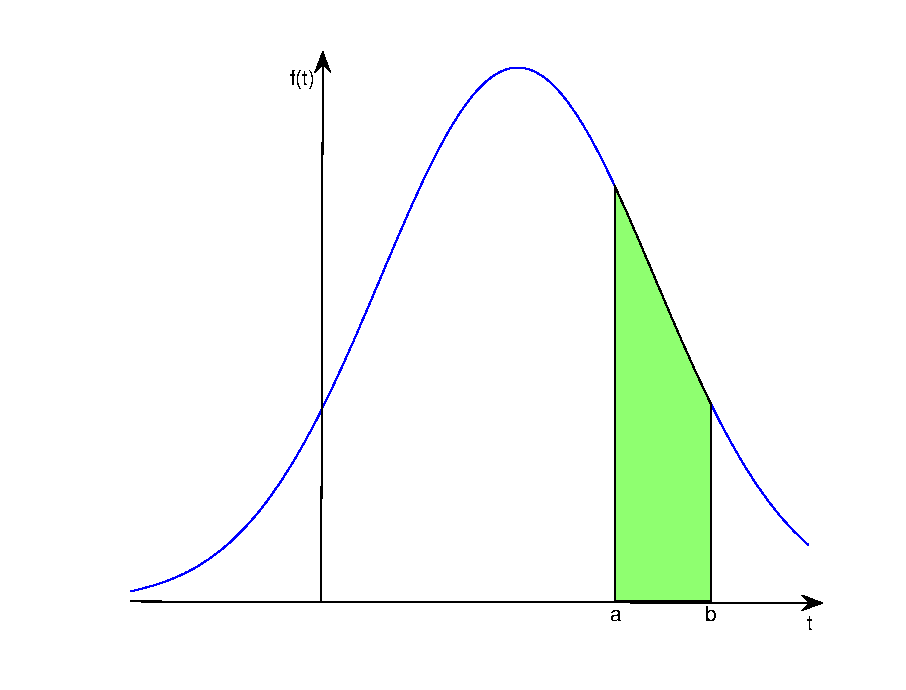
\includegraphics[width=0.6\textwidth]{residence_time/distrib_a_b}
\end{center}
}

\frame{\frametitle{Cumulative distribution function}
The cumulative distribution function (c.d.f.) is a function $F(t)$ that characterizes the distribution of $T$, and defined by
\[
F(s)=\Proba{T\leq s}=\int_{-\infty}^sf(x)dx.
\]
\begin{center}
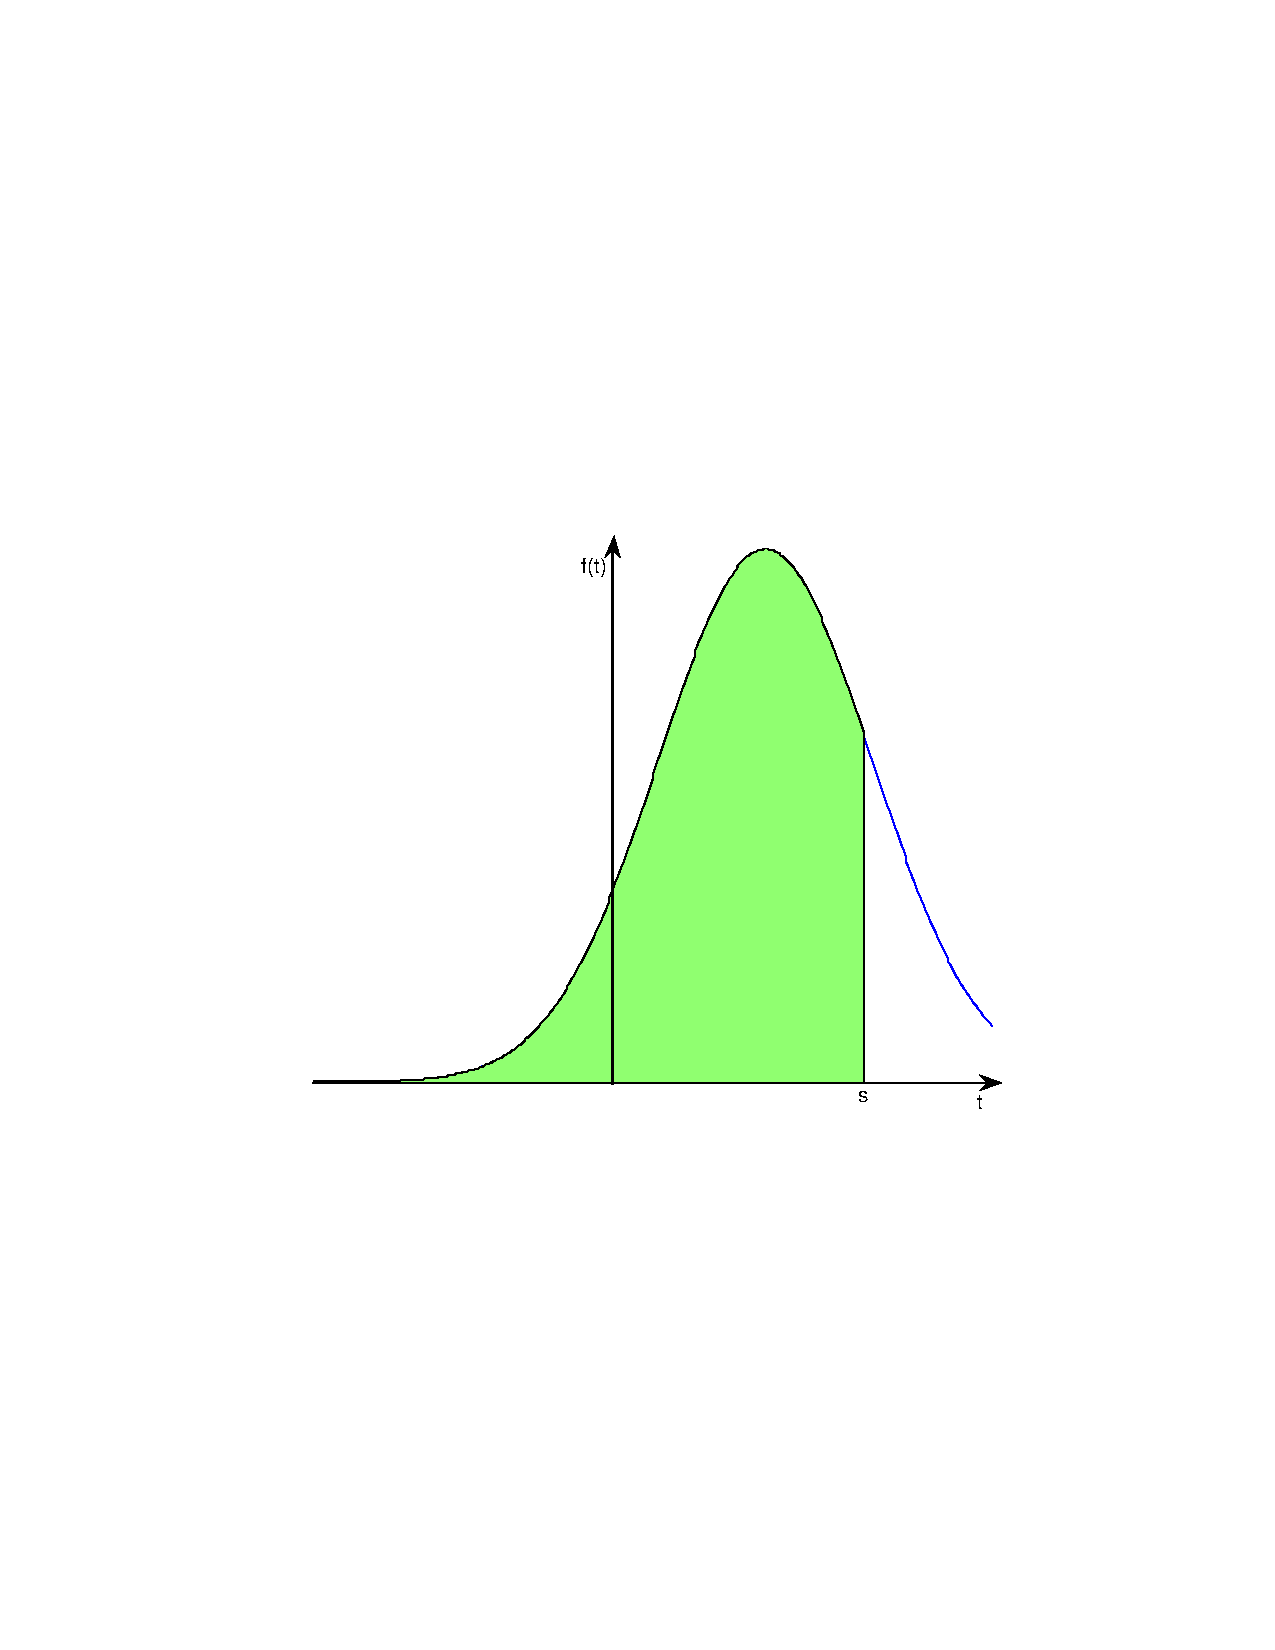
\includegraphics[width=0.6\textwidth]{residence_time/cdf_auc}
\end{center}
}

\frame{\frametitle{Properties of the c.d.f.}
\begin{itemize}
\item
Since $f$ is a nonnegative function, $F$ is nondecreasing.
\item
Since $f$ is a probability density function, $\int_{-\infty}^{+\infty}f(s)ds=1$, and thus $\lim_{t\to\infty}F(t)=1$.
\end{itemize}
\begin{center}
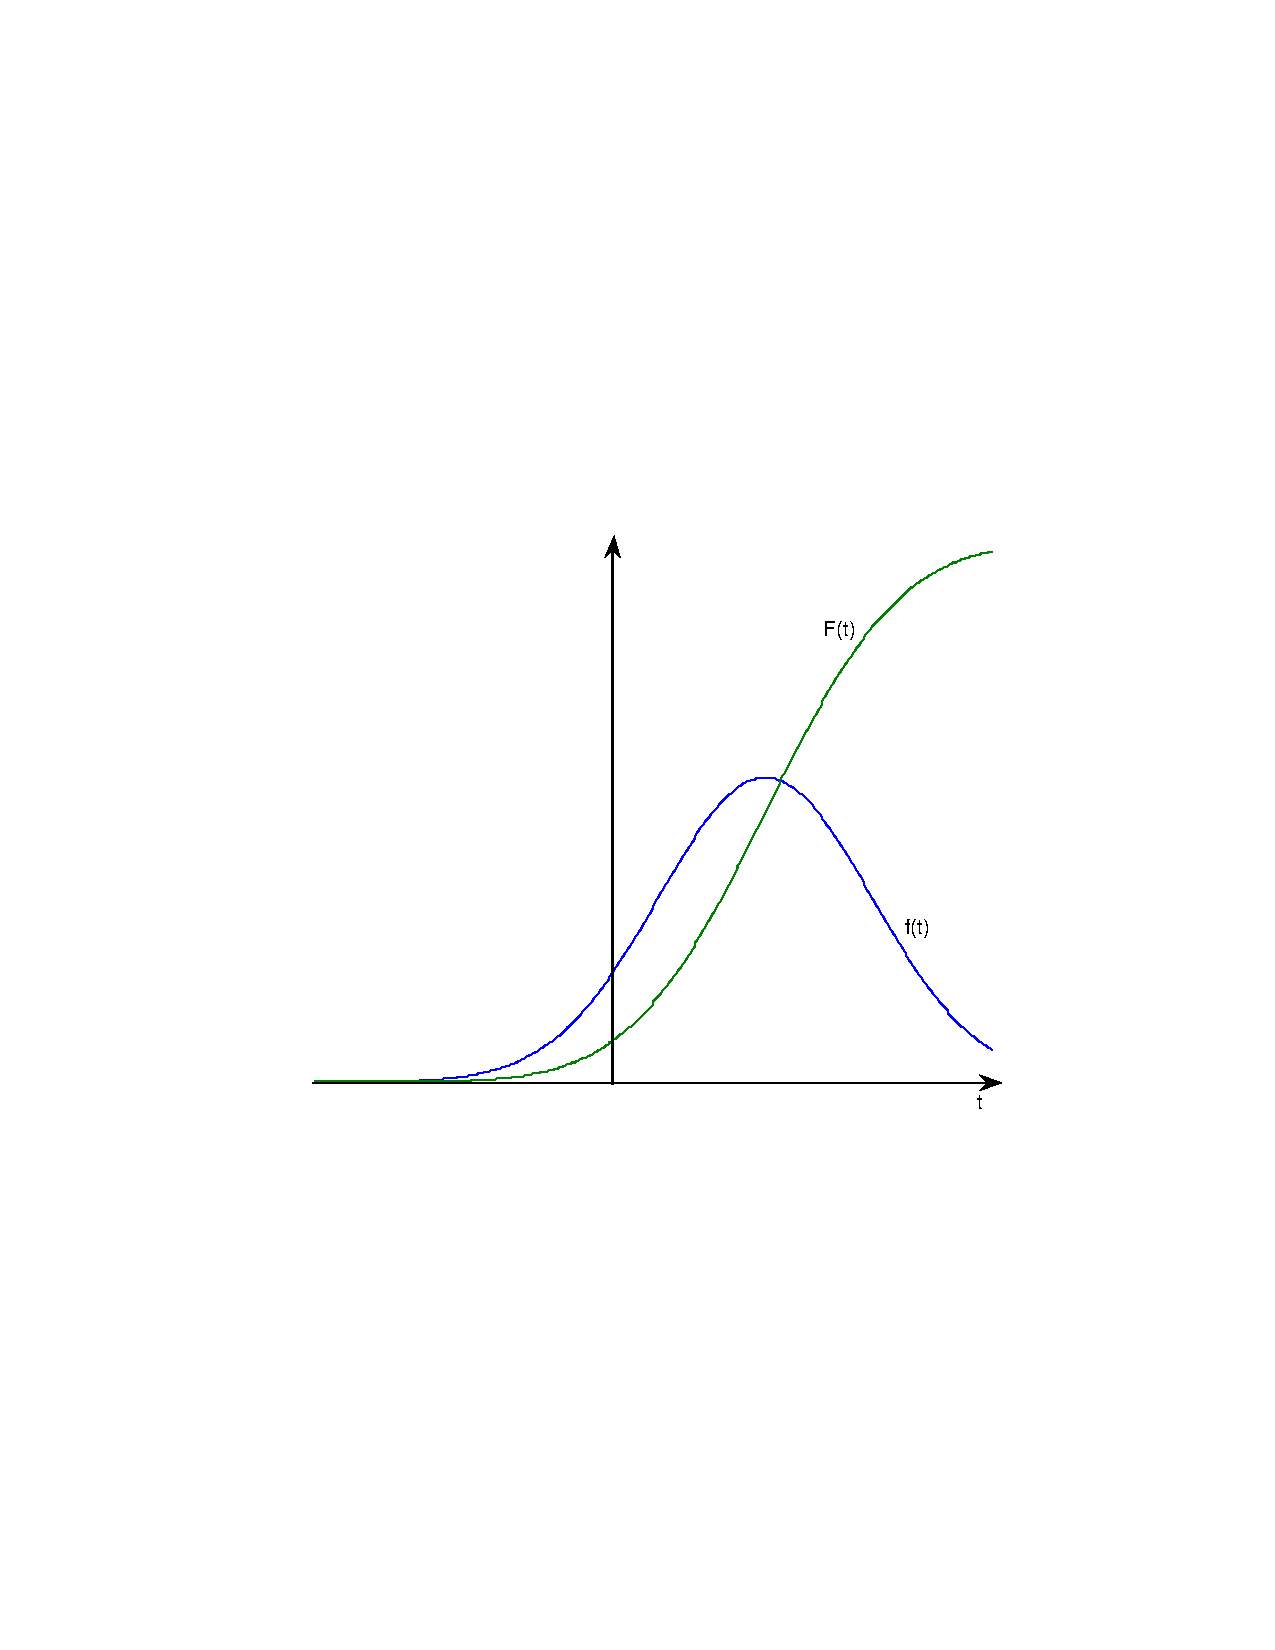
\includegraphics[width=0.6\textwidth]{residence_time/cdf_plot}
\end{center}
}

\frame{\frametitle{Mean value}
For a continuous random variable $T$ with probability density function $f$, the \emph{mean} value of $T$, denoted $\bar T$ or $E(T)$, is given by
\[
E(T)=\int_{-\infty}^{+\infty} tf(t)dt.
\]
}


\frame{\frametitle{Survival function}
Another characterization of the distribution of the random variable
$T$ is through the \emph{survival} (or \emph{sojourn}) function. 

\vskip1cm
The survival function of state $S_1$ is given by 
\begin{equation}
  \Surv(t)=1-F(t)=\Proba{T>t}
  \label{eq:survival}
\end{equation}
This gives a description of the \emph{sojourn time} of a
system in a particular state (the time spent in the state).
\vskip1cm
$\Surv$ is a nonincreasing function (since $\Surv=1-F$
with $F$ a c.d.f.), and
$\Surv(0)=1$ (since $T$ is a positive random variable).
}

\frame{
The \emph{average sojourn time} $\tau$ in state $S_1$ is given by
\[
\tau=E(T)=\int_0^\infty tf(t)dt
\]
Assuming that $\lim_{t\to\infty}t\Surv(t)=0$ (which is verified
for most probability distributions), 
\[
\tau=\int_0^\infty \Surv(t)dt
\]
}

%%%%%%%%%%%%%%
%%%%%%%%%%%%%%
%%%%%%%%%%%%%%
%%%%%%%%%%%%%%
\section{Markov chains}

\frame{
We conduct an experiment with a set of $r$ outcomes,
\[
S=\{S_1,\dots, S_r\}.
\]
\vskip0.4cm
The experiment is repeated $n$ times (with $n$ large, potentially infinite). 
\vskip0.4cm
The system has \underline{no memory}: the next state depends only on the present state. 
\vskip0.4cm
The probability of $S_j$ occurring on the next step, given that $S_i$ occurred on the last step, is
\[
p_{ij}=p(S_j|S_i).
\]
}

\frame{\frametitle{Markov chain}
\begin{definition}
An experiment with finite number of possible outcomes $S_1,\ldots,S_r$ is repeated. The sequence of outcomes is a \emph{Markov chain} if there is a set of $r^2$ numbers $\{p_{ij}\}$ such that the conditional probability of outcome $S_j$ on any experiment given outcome $S_i$ on the previous experiment is $p_{ij}$, i.e., for $1\leq i,j\leq r$, $n=1,\ldots$,
\[
p_{ij}=\mathsf{Pr}(S_j\textrm{ on experiment }n+1|S_i\textrm{ on experiment }n).
\]
The outcomes $S_1,\ldots,S_r$ are the \emph{states}, and the $p_{ij}$ are the \emph{transition probabilities}. The matrix $P=[p_{ij}]$ is the \emph{transition matrix}.
\end{definition}
}

\frame{\frametitle{Transition matrix}
The matrix 
\[
P=
\begin{pmatrix}
p_{11} & p_{12} & \cdots & p_{1r} \\
p_{21} & p_{22} & \cdots & p_{2r} \\
&&& \\
p_{r1} & p_{r2} & \cdots & p_{rr}
\end{pmatrix}
\]
has
\begin{itemize}
\item nonnegative entries, $p_{ij}\geq 0$
\item entries less than 1, $p_{ij}\leq 1$
\item row sum 1, which we write
\[
\sum_{j=1}^r p_{ij}=1,\quad i=1,\ldots,r
\]
or, using the notation $\nbOne^T=(1,\ldots,1)$,
\[
P\nbOne=\nbOne
\]
\end{itemize}
}


\frame{\frametitle{Repetition of the process}
Let $p_i(n)$ be the probability that the state $S_i$ will occur on the $n^{th}$ repetition of the experiment, $1\leq i\leq r$. Then
\begin{equation}
p(n+1)=p(n)P, \quad n=1,2,3,\dots
\end{equation}
where $p(n)=(p_1(n),p_{2}(n),\dots , p_r(n))$ is a (row) probability vector and $P=(p_{ij})$ is a $r\times r$ \emph{transition matrix},
\[
P=
\begin{pmatrix}
p_{11} & p_{12} & \cdots & p_{1r} \\
p_{21} & p_{22} & \cdots & p_{2r} \\
&&& \\
p_{r1} & p_{r2} & \cdots & p_{rr}
\end{pmatrix}
\]
}

\frame{\frametitle{Stochastic matrices}
\begin{definition}[Stochastic matrix]
The nonnegative $r\times r$ matrix $M$ is \emph{stochastic} if $\sum_{j=1}^ra_{ij}=1$ for all $i=1,2,\dots, r$.
\end{definition}
\begin{theorem}
Let $M$ be a stochastic matrix $M$. Then all eigenvalues $\lambda$ of $M$ are such that $|\lambda|\leq 1$. 
Furthermore, $\lambda =1$ is an eigenvalue of $M$.
\end{theorem}
\vskip0.4cm
To see that $1$ is an eigenvalue, write the definition of a stochastic matrix, i.e., $M$ has row sums 1. In vector form, $M\nbOne=\nbOne$. Now remember that $\lambda$ is an eigenvalue of $M$, with associated eigenvector $v$, iff $Mv=\lambda v$. So, in the expression $M\nbOne=\nbOne$, we read an eigenvector, $\nbOne$, and an eigenvalue, $1$.
}

\frame{\frametitle{Long ``time'' behavior}
Let $p(0)$ be the initial distribution (row) vector. Then
\begin{align*}
p(1) &= p(0)P \\
p(2) &= p(1)P\\
&= (p(0)P)P \\
&= p(0)P^2
\end{align*}
Iterating, we get that for any $n$,
\[
p(n)=p(0)P^n
\]
Therefore, 
\[
\lim_{n\rightarrow +\infty}p(n)=\lim_{n\rightarrow +\infty}p(0)P^n=p(0)\lim_{n\rightarrow +\infty}P^n
\]
}

\frame{\frametitle{Additional properties of stochastic matrices}
\begin{theorem}
If $M,N$ are stochastic matrices, then $MN$ is a stochastic matrix.
\end{theorem}
\begin{theorem}
If $M$ is a stochastic matrix, then for any $k\in\IN$, $M^k$ is a stochastic matrix.
\end{theorem}
}

\subsection{Regular Markov chains}


\frame{\frametitle{Regular Markov chain}
\begin{definition}[Regular Markov chain]
A regular Markov chain is one in which $P^k$ is positive for some integer $k>0$, i.e., $P^k$ has only positive entries, no zero entries.
\end{definition}
\begin{definition}
A nonnegative matrix $M$ is primitive if, and only if, there is an integer $k>0$ such that $M^k$ is positive.
\end{definition}
\begin{theorem}
A Markov chain is regular if, and only if, the transition matrix $P$ is primitive.
\end{theorem}
}

\frame{\frametitle{Important result for regular Markov chains}
\begin{theorem}
If $P$ is the transition matrix of a regular Markov chain, then
\begin{enumerate}
\item the powers $P^n$ approach a stochastic matrix $W$,
\item each row of $W$ is the same (row) vector $w=(w_1,\ldots,w_r)$,
\item the components of $w$ are positive.
\end{enumerate}
\end{theorem}
So if the Markov chain is regular,
\[
\lim_{n\rightarrow +\infty}p(n)=p(0)\lim_{n\rightarrow +\infty}P^n
=p(0)W
\]
}


\frame{\frametitle{Left and right eigenvectors}
Let $M$ be an $r\times r$ matrix, $u,v$ be two column vectors, $\lambda\in\IR$. Then, if  
\[
Mu=\lambda u,
\]
$u$ is the (right) eigenvector corresponding to $\lambda$, and if
\[
v^TM=\lambda v^T
\]
then $v$ is the left eigenvector corresponding to $\lambda$. Note that to a given eigenvalue there corresponds one left and one right eigenvector.
}

\frame{
The vector $w$ is in fact the left eigenvector corresponding to the eigenvalue 1 of $P$. (We already know that the (right) eigenvector corresponding to 1 is $\nbOne$.)
\vskip0.5cm
To see this, remark that, if $p(n)$ converges, then $p(n+1)=p(n)P$, so $w$ is a fixed point of the system. We thus write
\[
wP=w
\]
and solve for $w$, which amounts to finding $w$ as the left eigenvector corresponding to the eigenvalue 1.
\vskip0.5cm
Alternatively, we can find $w$ as the (right) eigenvector associated to the eigenvalue 1 for the transpose of $P$,
\[
P^Tw^T=w^T
\]
}

\frame{
Now remember that when you compute an eigenvector, you get a result that is the eigenvector, to a multiple.
\vskip1cm
So the expression you obtain for $w$ might have to be normalized (you want a probability vector). Once you obtain $w$, check that the norm $\|w\|$ defined by
\[
\|w\|=w_1+\cdots+w_r
\]
is equal to one. If not, use
\[
\frac{w}{\|w\|}
\]
}


\subsection{Absorbing Markov chains}

\frame{\frametitle{Absorbing states, absorbing chains}
\begin{definition}
A state $S_i$ in a Markov chain is \emph{absorbing} if whenever it occurs on the $n^{th}$ generation of the experiment, it then occurs on every subsequent step. In other words, $S_i$ is absorbing if $p_{ii}=1$ and $p_{ij}=0$ for $i\neq j$.
\end{definition}

\begin{definition}
A Markov chain is said to be absorbing if it has at least one absorbing state, and if from every state it is possible to go to an absorbing state.
\end{definition}

In an absorbing Markov chain, a state that is not absorbing is called \emph{transient}.
}


\frame{\frametitle{Some questions on absorbing chains}
Suppose we have a chain like the following:
\begin{center}
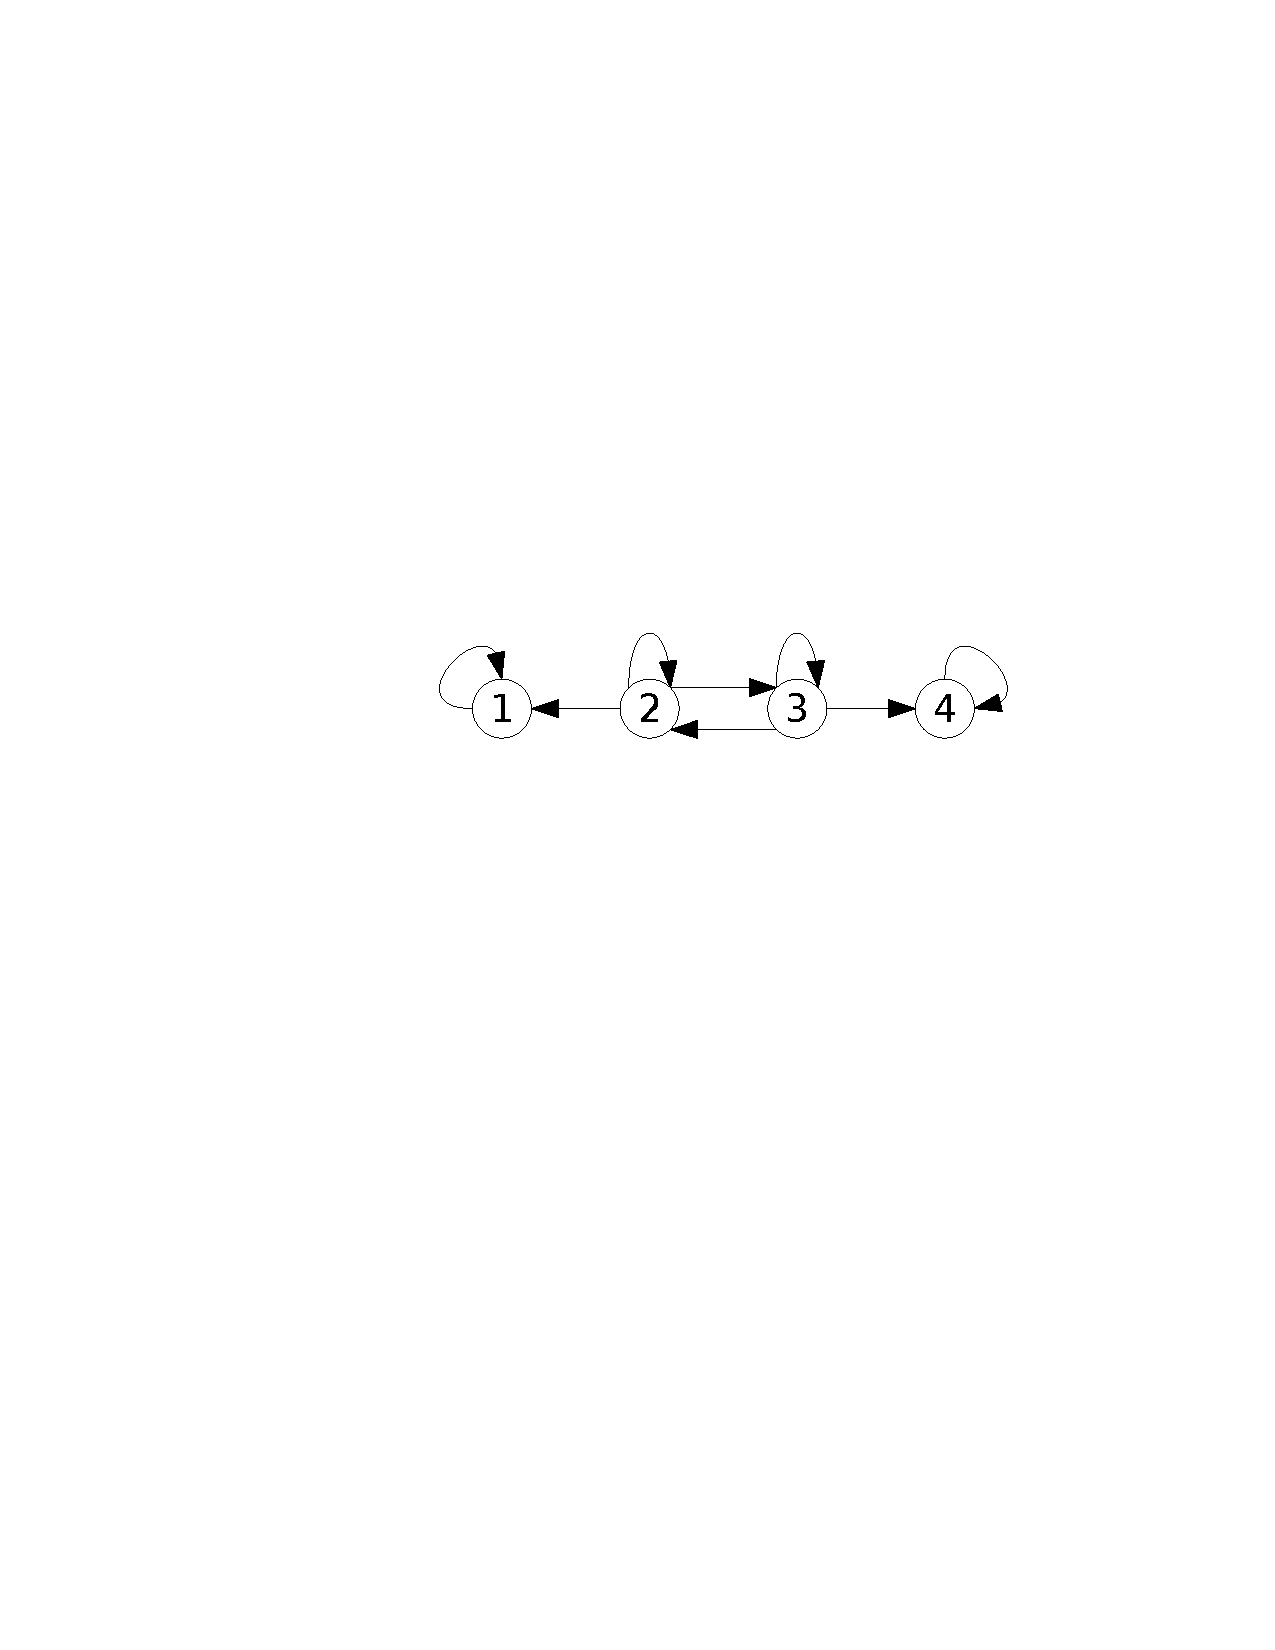
\includegraphics[width=0.8\textwidth]{genetics/graphe_absorbant}
\end{center}
\begin{enumerate}
\item Does the process eventually reach an absorbing state?
\item Average number of times spent in a transient state, if starting in a transient state?
\item Average number of steps before entering an absorbing state?
\item Probability of being absorbed by a given absorbing state, when there are more than one, when starting in a given transient state?
\end{enumerate}
}

\frame{\frametitle{Reaching an absorbing state}
Answer to question 1:
\begin{theorem}
In an absorbing Markov chain, the probability of reaching an absorbing state is 1.
\end{theorem}
}

\frame{\frametitle{Standard form of the transition matrix}
For an absorbing chain with $k$ absorbing states and $r-k$ transient states, the transition matrix can be written as
\[
P=\begin{pmatrix}
\mathbb{I}_k & \mathbf{0} \\
R & Q
\end{pmatrix}
\]
with following meaning,
\begin{center}
\begin{tabular}{ccc}
& Absorbing states & Transient states \\
Absorbing states & $\mathbb{I}_k$ & $\mathbf{0}$ \\
Transient states & $R$ & $Q$
\end{tabular}
\end{center}
with $\mathbb{I}_k$ the $k\times k$ identity matrix, $\mathbf{0}$ an $k\times(r-k)$ matrix of zeros, $R$ an $(r-k)\times k$ matrix and $Q$ an $(r-k)\times(r-k)$ matrix.
}

\frame{
The matrix $\mathbb{I}_{r-k}-Q$ is invertible. Let
\begin{itemize}
\item $N=(\mathbb{I}_{r-k}-Q)^{-1}$ be the \emph{fundamental matrix} of the Markov chain
\item $T_i$ be the sum of the entries on row $i$ of $N$
\item $B=NR$.
\end{itemize}
\vskip0.5cm
Answers to our remaining questions:
\begin{enumerate}
\setcounter{enumi}{1}
\item $N_{ij}$ is the average number of times the process is in the $j$th transient state if it starts in the $i$th transient state.
\item $T_i$ is the average number of steps before the process enters an absorbing state if it starts in the $i$th transient state.
\item $B_{ij}$ is the probability of eventually entering the $j$th absorbing state if the process starts in the $i$th transient state.
\end{enumerate}
}




%%%%%%%%%%%%%%
%%%%%%%%%%%%%%
%%%%%%%%%%%%%%
%%%%%%%%%%%%%%
%%%%%%%%%%%%%%
%%%%%%%%%%%%%%
%%%%%%%%%%%%%%
%%%%%%%%%%%%%%
\part{Modelling topics}

\frame{\frametitle{Modelling topics}
\tableofcontents[part=2,hideallsubsections]
}


%%%%%%%%%%%%%%
%%%%%%%%%%%%%%
%%%%%%%%%%%%%%
%%%%%%%%%%%%%%
\section{Single population dynamics and the logistic situation}

\subsection{The data: US census}

\frame{\frametitle{The US population from 1790 to 1910}
\begin{center}
\begin{tabular}[t]{cc}
\begin{tabular}{cc}
Year & Population\\
& (millions) \\
\hline
1790 & 3.929 \\
1800 & 5.308 \\
1810 & 7.240 \\
1820 & 9.638 \\
1830 & 12.866 \\
1840 & 17.069 \\
1850 & 23.192
\end{tabular} 
&
\begin{tabular}{cc}
Year & Population \\
& (millions) \\
\hline
1860 & 31.443 \\
1870 & 38.558 \\
1880 & 50.156 \\
1890 & 62.948 \\
1900 & 75.995 \\
1910 & 91.972 
\end{tabular}
\end{tabular}
\end{center}
}


\frame{
\begin{center}
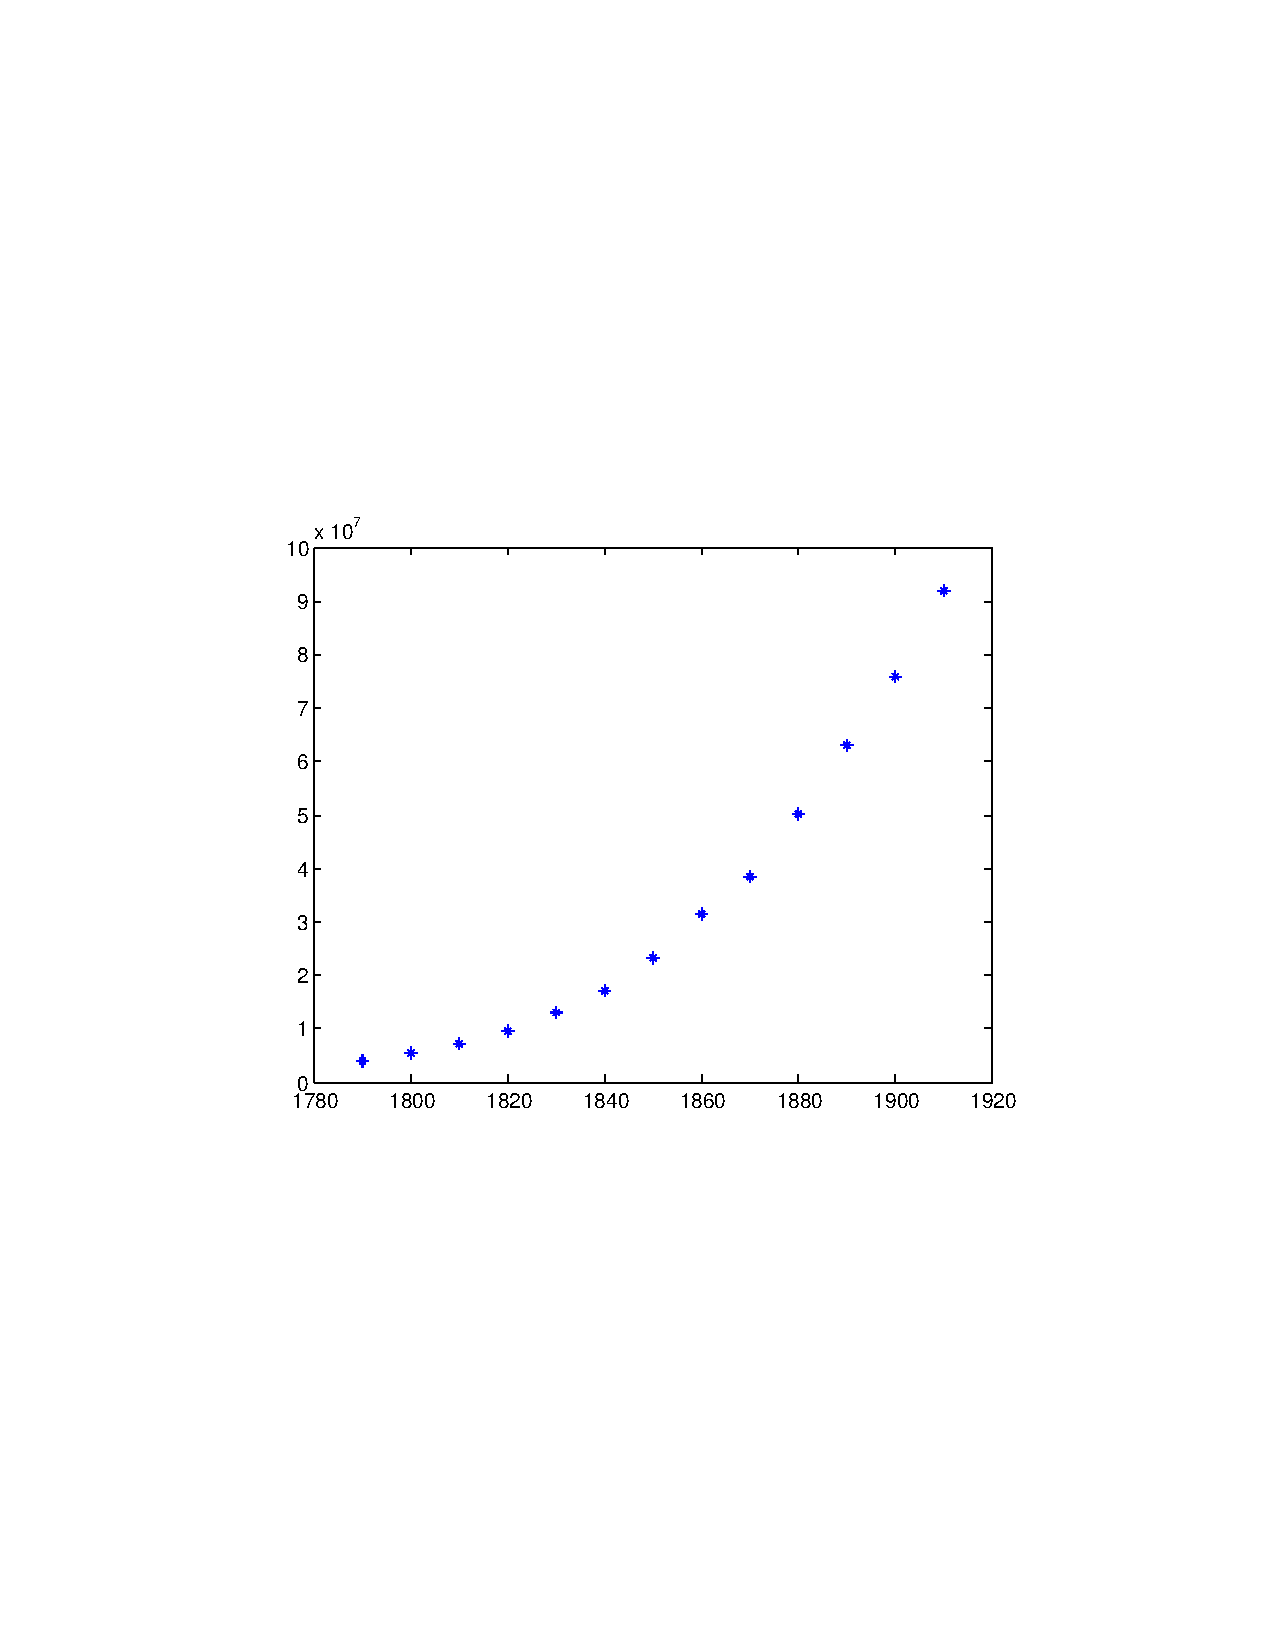
\includegraphics[width=0.9\textwidth]{population_growth/USpop_to1910_points}
\end{center}
}

\subsection{A quadratic curve?}

\frame{\frametitle{First idea}
The curve looks like a piece of a parabola. So let us fit a curve of the form
\[
P(t)=a+bt+ct^2.
\]
To do this, we want to minimize
\[
S=\sum_{k=1}^{13} \left(P(t_k)-P_k\right)^2,
\]
where $t_k$ are the known dates, $P_k$ are the known populations, and $P(t_k)=a+bt_k+ct_k^2$.
}

\frame{\frametitle{Our first guess, in pictures}
\begin{center}
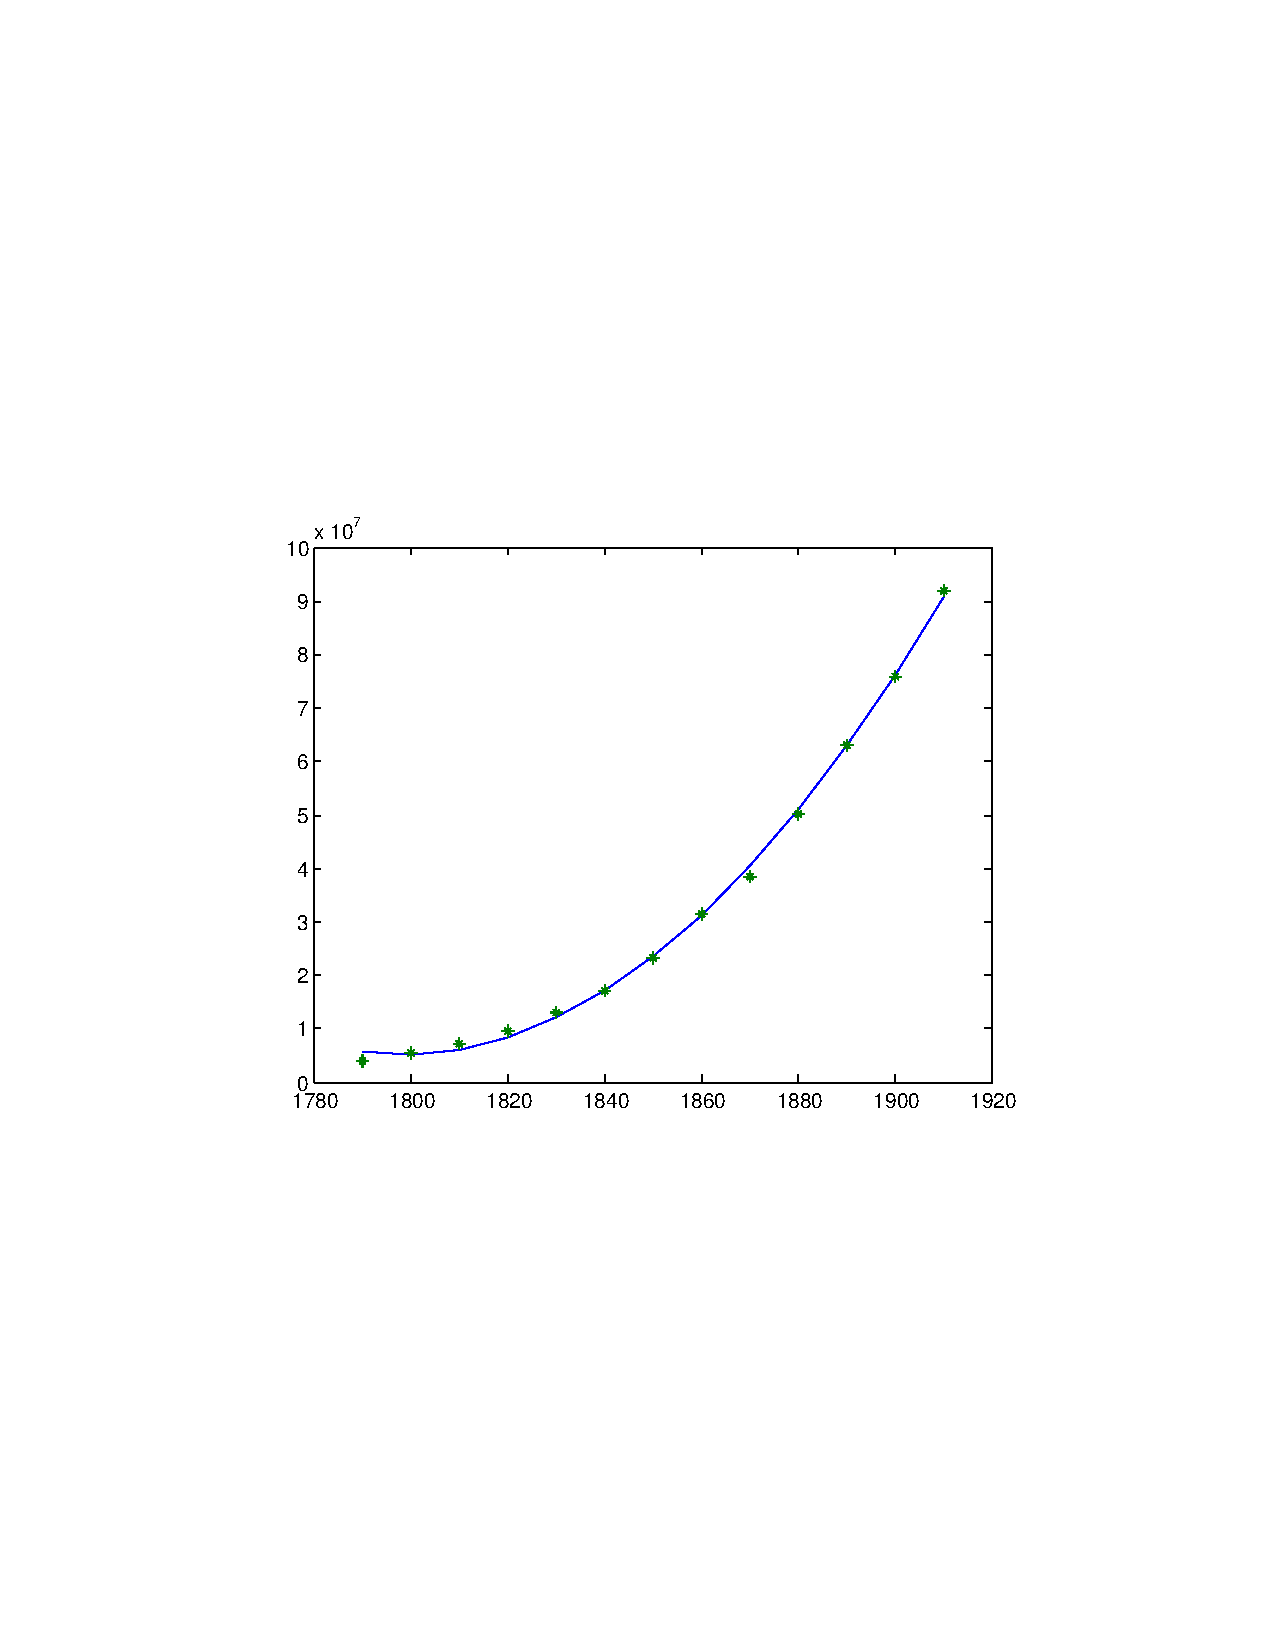
\includegraphics[width=0.9\textwidth]{population_growth/quadratic_fit}
\end{center}
}


\frame[containsverbatim]{\frametitle{which turned out to work quite well}
How does our formula do for present times?
\begin{verbatim}
f(2006)
ans =     301468584.066013
\end{verbatim}
301,468,584, compared to the 298,444,215 July 2006 estimate, overestimates the population by 3,024,369, a relative error of approximately 1\%.
}

\subsection{Population growth -- Logistic equation}

\frame{\frametitle{The logistic equation}
The logistic curve is the solution to the ordinary differential equation
\[
N'=rN\left(1-\frac NK\right),
\]
which is called the \emph{logistic equation}. $r$ is the \emph{intrinsic growth rate}, $K$ is the \emph{carrying capacity}.
\vskip1cm
This equation was introduced by Pierre-Fran\c{c}ois Verhulst (1804-1849), in 1844.
}

\frame{\frametitle{Reinterpreting the logistic equation}
The equation
\[
N'=bN-dN-cN^2
\]
is rewritten as
\[
N'=(b-d)N-cN^2.
\]
\begin{itemize}
\item $b-d$ represents the rate at which the population increases (or decreases) in the absence of competition. It is called the \emph{intrinsic growth rate} of the population.
\item $c$ is the rate of \emph{intraspecific} competition. The prefix \emph{intra} refers to the fact that the competition is occurring between members of the same species, that is, within the species.
\end{itemize}
}


\frame{\frametitle{Equivalent equations}
\begin{align*}
N' &= (b-d)N-cN^2\\
&= \bigl((b-d)-cN\bigr)N \\
&= \left(r-\frac rr cN\right)N,\quad\textrm{with }r=b-d \\
&= rN\left(1-\frac crN\right) \\
&= rN\left(1-\frac NK\right),
\end{align*}
with
\[
\frac cr=\frac 1K,
\]
that is, $K=r/c$.
}

\subsection{Qualitative analysis of the logistic ODE}

\frame{\frametitle{Studying the logistic equation qualitatively}
We study
\begin{equation}\label{eq:logistic_ode}
N'=rN\left(1-\frac NK\right).\tag{ODE1}
\end{equation}
For this, write
\[
f(N)=rN\left(1-\frac NK\right).
\]
Consider the initial value problem (IVP) 
\begin{equation}\label{ivp:logistic_ode}
N'=f(N),\quad N(0)=N_0>0.\tag{IVP1}
\end{equation}
\begin{itemize}
\item $f$ is $C^1$ (differentiable with continuous derivative) so solutions to \eqref{ivp:logistic_ode} exist and are unique.
\end{itemize}
}

\frame{
\emph{Equilibria} of \eqref{eq:logistic_ode} are points such that $f(N)=0$ (so that $N'=f(N)=0$, meaning $N$ does not vary). So we solve $f(N)=0$ for $N$. We find two points:
\begin{itemize}
\item $N=0$
\item $N=K$.
\end{itemize}
By uniqueness of solutions to \eqref{ivp:logistic_ode}, solutions cannot cross the lines $N(t)=0$ and $N(t)=K$.
}

\frame{
There are several cases.
\begin{itemize}
\item $N=0$ for some $t$, then $N(t)=0$ for all $t\geq 0$, by uniqueness of solutions.
\item $N\in(0,K)$, then $rN>0$ and $N/K<1$ so $1-N/K>0$, which implies that $f(N)>0$. As a consequence, $N(t)$ increases if $N\in(0,K)$.
\item $N=K$, then $rN>0$ but $N/K=1$ so $1-N/K=0$, which implies that $f(N)=0$. As a consequence, $N(t)=K$ for all $t\geq 0$, by uniqueness of solutions.
\item $N>K$, the $rN>0$ and $N/K>1$, implying that $1-N/K<0$ and in turn, $f(N)<0$. As a consequence, $N(t)$ decreases if $N\in(K,+\infty)$.
\end{itemize}
}

\frame{
Therefore,
\begin{theorem}
Suppose that $N_0>0$. Then the solution $N(t)$ of \eqref{ivp:logistic_ode} is such that
\[
\lim_{t\to\infty} N(t)=K,
\]
so that $K$ is the number of individuals that the environment can support, the \emph{carrying capacity} of the environment.

If $N_0=0$, then $N(t)=0$ for all $t\geq 0$.
\end{theorem}
}


\subsection{The delayed logistic equation}
\frame{\frametitle{The delayed logistic equation}
Consider the equation as
\[
\frac{N'}{N}=(b-d)-cN,
\]
that is, the per capita rate of growth of the population depends on the net growth rate $b-d$, and some density dependent inhibition $cN$ (resulting of competition).

Suppose that instead of instantaneous inhibition, there is some delay $\tau$ between the time the inhibiting event takes place and the moment where it affects the growth rate. (For example, two individuals fight for food, and one later dies of the injuries sustained when fighting).
}

\frame{\frametitle{The delay logistic equation}
In the of a time $\tau$ between inhibiting event and inhibition, the equation would be written as
\[
\frac{N'}N=(b-d)-cN(t-\tau).
\]
Using the change of variables introduced earlier, this is written
\begin{equation}\label{eq:logistic_dde}
N'(t)=rN(t)\left(1-\frac{N(t-\tau)}K\right). \tag{DDE1}
\end{equation}
Such an equation is called a \emph{delay} differential equation. It is much more complicated to study than \eqref{eq:logistic_ode}. In fact, some things remain unknown about \eqref{eq:logistic_dde}.
}

\frame{\frametitle{Delayed initial value problem}
The IVP takes the form
\begin{equation}\label{ivp:logistic_dde}
\begin{aligned}
N'(t)&= rN(t)\left(1-\frac{N(t-\tau)}K\right),\\
N(t) &= \phi(t)\textrm{ for }t\in[-\tau,0],
\end{aligned} \tag{IVP2}
\end{equation}
where $\phi(t)$ is some continuous function. Hence, initial conditions (called initial data in this case) must be specific on an interval, instead of being specified at a point, to guarantee existence and uniqueness of solutions.

We will not learn how to study this type of equation (this is graduate level mathematics). I will give a few results.
}

\frame{
To find equilibria, remark that delay should not play a role, since $N$ should be constant. Thus, equilibria are found by considering the equation with no delay, which is \eqref{eq:logistic_ode}.
\begin{theorem}
Suppose that $r\tau<22/7$. Then all solutions of \eqref{ivp:logistic_dde} with positive initial data $\phi(t)$ tend to $K$. If $r\tau>\pi/2$, then $K$ is an unstable equilibrium and all solutions of \eqref{ivp:logistic_dde} with positive initial data $\phi(t)$ on $[-\tau,0]$ are oscillatory.
\end{theorem}
\vskip1cm
Note that there is a gray zone between $22/7$ and $\pi/2$.. The first part of the theorem was proved in 1945 by Wright. Although there is very strong numerical evidence that this is in fact true up to $\pi/2$, nobody has yet managed to prove it.
}

\subsection{The logistic map}

\frame{\frametitle{The logistic map}
The logistic \emph{map} is, for $t\geq 0$,
\begin{equation}\label{eq:logistic_discrete}
N_{t+1}=rN_t\left(1-\frac{N_t}K\right). \tag{DT1}
\end{equation}
To transform this into an initial value problem, we need to provide an initial condition $N_0\geq 0$ for $t=0$.
}


\frame{
Consider the simplified version \eqref{eq:logistic_discrete_scaled},
\[
x_{t+1}=rx_t(1-x_t)\stackrel{\Delta}{=}f_r(x_t).
\]
{\bf Are solutions well defined?}
Suppose $x_0\in[0,1]$, do we stay in $[0,1]$? 
$f_r$ is continuous on $[0,1]$, so it has a extrema on $[0,1]$. We have
\[
f_r'(x)=r-2rx=r(1-2x),
\]
which implies that $f_r$ increases for $x<1/2$ and decreases for $x>1/2$, reaching a maximum at $x=1/2$. 
\vskip0.5cm
$f_r(0)=f_r(1)=0$ are the minimum values, and $f(1/2)=r/4$ is the maximum. Thus, if we want $x_{t+1}\in[0,1]$ for $x_t\in[0,1]$, we need to consider $r\leq 4$.
}

\frame{
\begin{itemize}
\item Note that if $x_0=0$, then $x_t=0$ for all $t\geq 1$. 
\item Similarly, if $x_0=1$, then $x_1=0$, and thus $x_t=0$ for all $t\geq 1$.
\item This is true for all $t$: if there exists $t_k$ such that $x_{t_k}=1$, then $x_t=0$ for all $t\geq t_k$.
\item This last case might occur if $r=4$, as we have seen.
\item Also, if $r=0$ then $x_t=0$ for all $t$.
\end{itemize}
For these reasons, we generally consider
\[
x\in(0,1)
\]
and
\[
r\in(0,4).
\]
}

\frame{\frametitle{Fixed points: existence}
{\bf Fixed points} of \eqref{eq:logistic_discrete_scaled} satisfy $x=rx(1-x)$, giving:
\begin{itemize}
\item $x=0$;
\item $1=r(1-x)$, that is, $p\stackrel{\Delta}{=}\dfrac{r-1}{r}$. 
\end{itemize}
Note that $\lim_{r\to 0^+}p=1-\lim_{r\to 0^+}1/r=-\infty$, $\frac{\partial}{\partial r}p=1/r^2>0$ (so $p$ is an increasing function of $r$), $p=0\Leftrightarrow r=1$ and $\lim_{r\to\infty}p=1$. 
So we come to this first conclusion:
\begin{itemize}
\item 0 always is a fixed point of $f_r$.
\item If $0<r<1$, then $p$ tales negative values so is not relevant.
\item If $1<r<4$, then $p$ exists.
\end{itemize}
}


\frame{\frametitle{Stability of the fixed points}
{\bf Stability} of the fixed points is determined by the (absolute) value $f_r'$ at these fixed points. We have
\[
|f'_r(0)|=r,
\]
and
\begin{align*}
|f'_r(p)| &= \left|r-2r\dfrac{r-1}{r}\right|\\
&= |r-2(r-1)| \\
&= |2-r|
\end{align*}
Therefore, we have
\begin{itemize}
\item if $0<r<1$, then the fixed point $x=p$ does not exist and $x=0$ is attracting,
\item if $1<r<3$, then $x=0$ is repelling, and $x=p$ is attracting,
\item if $r>3$, then $x=0$ and $x=p$ are repelling.
\end{itemize}
}

\frame{
\begin{center}
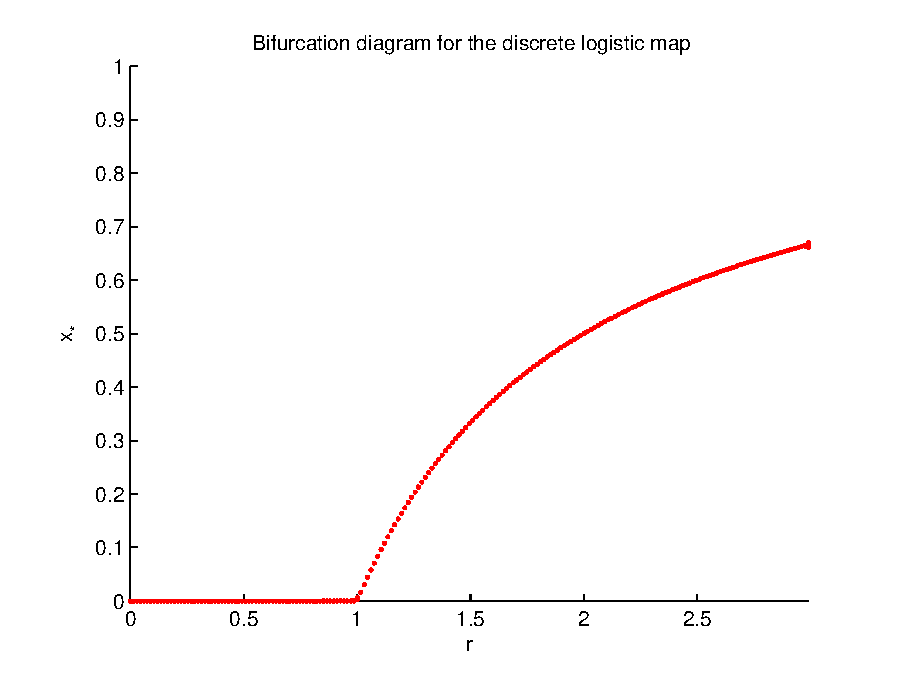
\includegraphics[width=0.9\textwidth]{population_growth/bif_cascade_1}
\end{center}
}


\frame{\frametitle{Another bifurcation}
Thus the points $r=1$ and $r=3$ are bifurcation points. To see what happens when $r>3$, we need to look for period 2 points.

\begin{align}
f_r^2(x) &= f_r(f_r(x)) \nonumber\\
&= r f_r(x)(1-f_r(x)) \nonumber\\
&= r^2 x(1-x)(1-r x(1-x)). \label{eq:f_mu_2_a}
\end{align}
0 and $p$ are points of period 2, since a fixed point $x^*$ of $f$ satisfies $f(x^*)=x^*$, and so, $f^2(x^*)=f(f(x^*))=f(x^*)=x^*$. 

This helps localizing the other periodic points. Writing the fixed point equation as
\[
Q(x)\stackrel{\Delta}{=}f_r^2(x)-x=0,
\]
we see that, since $0$ and $p$ are fixed points of $f_\mu^2$, they are roots of $Q(x)$. Therefore, $Q$ can be factorized as
\[
Q(x)=x(x-p)(-r^3x^2+Bx+C),
\]
}


\frame{
Substitute the value $(r-1)/r$ for $p$ in $Q$, develop $Q$ and \eqref{eq:f_mu_2_a} and equate coefficients of like powers gives
\begin{equation}\label{eq:Q}
Q(x)=x\left(x-\frac{r-1}{r}\right)\left(-r^3 x^2+r^2(r+1)x-r(r+1)\right).
\end{equation}
We already know that $x=0$ and $x=p$ are roots of \eqref{eq:Q}. So we search for roots of
\[
R(x):=-r^3 x^2+r^2(r+1)x-r(r+1).
\]
Discriminant is 
\begin{align*}
\Delta &=r^4(r+1)^2-4r^4(r+1)\\ 
&= r^4(r+1)(r+1-4)\\
&= r^4(r+1)(r-3). 
\end{align*}
Therefore, $R$ has distinct real roots if $r>3$.
Remark that for $r=3$, the (double) root is $p=2/3$. For $r>3$ but very close to 3, it follows from the continuity of $R$ that the roots are close to $2/3$.

}


\frame{
We use Descartes' rule of signs. 
\begin{itemize}
\item
$R$ has signed coefficients $-+-$, so 2 sign changes imlying 0 or 2 positive real roots. 
\item
$R(-x)$ has signed coefficients $---$, so no negative real roots. 
\item 
Since $\Delta>0$, the roots are real, and thus it follows that both roots are positive.
\end{itemize}
To show that the roots are also smaller than 1, consider the change of variables $z=x-1$. The polynomial $R$ is transformed into 
\begin{align*}
R_2(z) &= -r^3 (z+1)^2+r^2(r+1)(z+1)-r(r+1) \\
&= -r^3z^2+r^2(1-r)z-r.
\end{align*}
For $r>1$, the signed coefficients are $---$, so $R_2$ has no root $z>0$, implying in turn that $R$ has no root $x>1$.
}


\frame{\frametitle{Summing up}
\begin{itemize}
\item If $0<r<1$, then $x=0$ is attracting, $p$ does not exist and there are no period 2 points.
\item At $r=1$, there is a bifurcation (called a \emph{transcritical} bifurcation).
\item If $1<r<3$, then $x=0$ is repelling, $p$ is attracting, and there are no period 2 points.
\item At $r=3$, there is another bifurcation (called a \emph{period-doubling} bifurcation).
\item For $r>3$, both $x=0$ and $x=p$ are repelling, and there is a period 2 point.
\end{itemize}
}

\frame{
\begin{center}
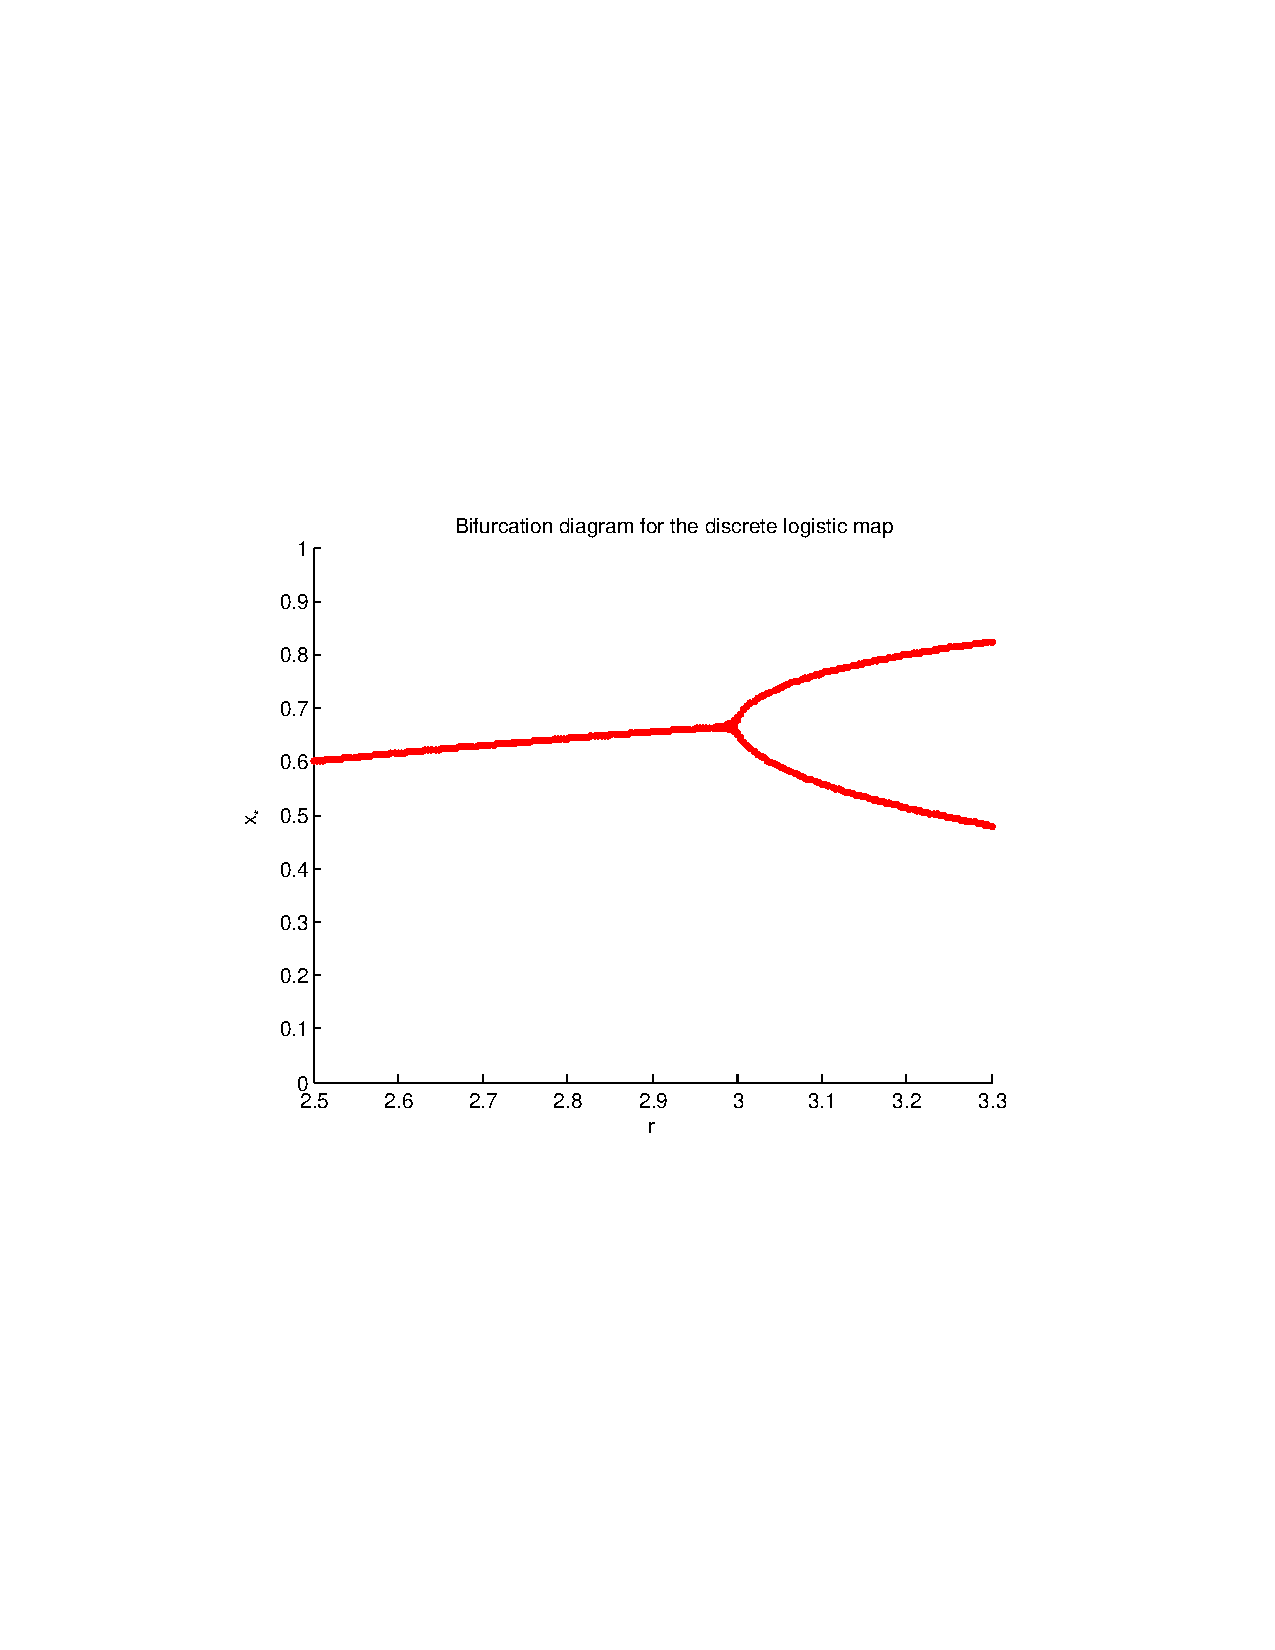
\includegraphics[width=0.9\textwidth]{population_growth/bif_cascade_2}
\end{center}
}
\frame{
\begin{center}
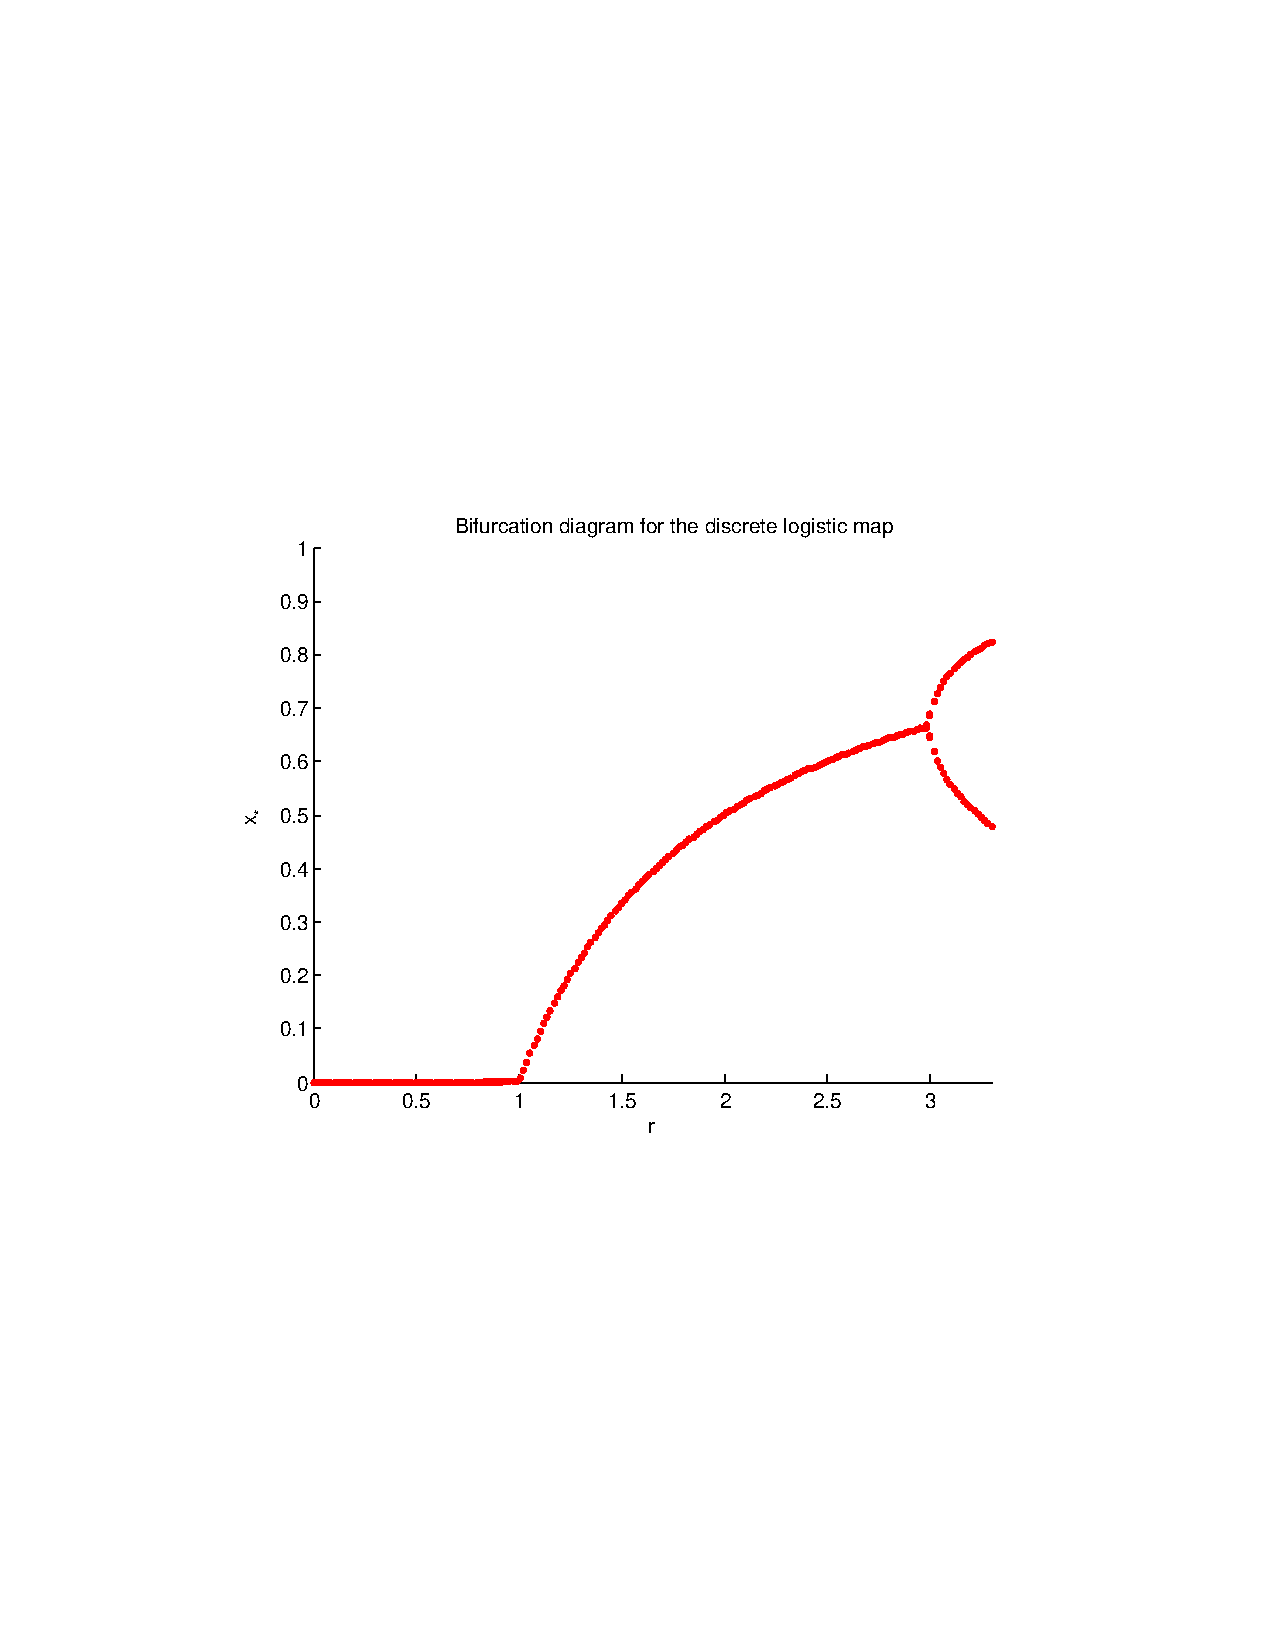
\includegraphics[width=0.9\textwidth]{population_growth/bif_cascade_3}
\end{center}
}


\frame{\frametitle{This process continues}
\begin{center}
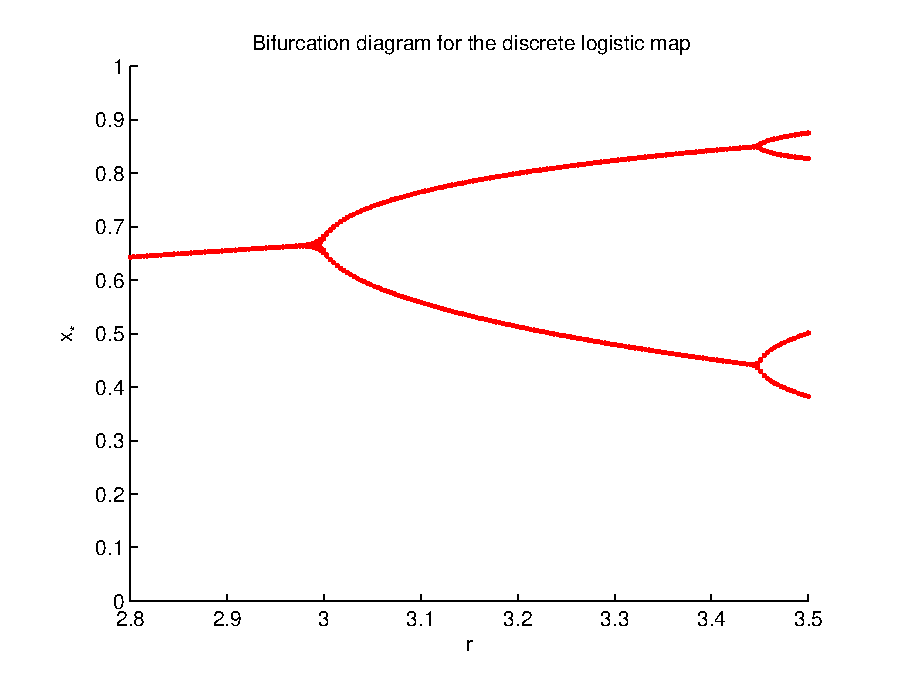
\includegraphics[width=0.9\textwidth]{population_growth/bif_cascade_4}
\end{center}
}

\frame{\frametitle{The period-doubling cascade to chaos}
The logistic map undergoes a sequence of period doubling bifurcations, called the \emph{period-doubling cascade}, as $r$ increases from 3 to 4.

\begin{itemize}
\item Every successive bifurcation leads to a doubling of the period.
\item The bifurcation points form a sequence, $\{r_n\}$, that has the property that
\[
\lim{n\to\infty}\frac{r_n-r_{n-1}}{r_{n+1}-r_n}
\]
exists and is a constant, called the Feigenbaum constant, equal to 4.669202\ldots
\item This constant has been shown to exist in many of the maps that undergo the same type of cascade of period doubling bifurcations.
\end{itemize}
}


\frame{
\begin{center}
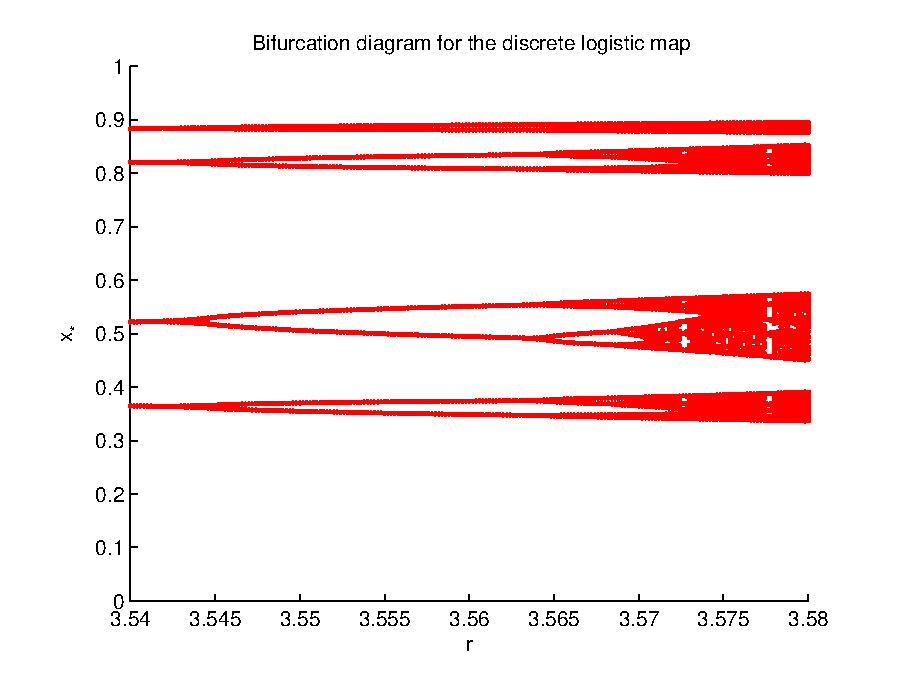
\includegraphics[width=0.9\textwidth]{population_growth/bif_cascade_5}
\end{center}
}

\frame{\frametitle{Chaos}
After a certain value of $r$, there are periodic points with all periods. In particular, there are periodic points of period 3. 
\vskip1cm
By a theorem (called the Sarkovskii theorem), the presence of period 3 points implies the presence of points of all periods.
\vskip1cm
At this point, the system is said to be in a \emph{chaotic regime}, or \emph{chaotic}.
}



%%%%%%%%%%%%%%
%%%%%%%%%%%%%%
%%%%%%%%%%%%%%
%%%%%%%%%%%%%%
\section{Time of residence in a state -- Exponential distribution}

\frame{\frametitle{The exponential distribution}
The random variable $T$ has an \emph{exponential} distribution if its probability density function takes the form
\begin{equation}\label{eq:exp_distrib}
f(t)=\begin{cases}0&\textrm{if }t<0,\\
\theta e^{-\theta t}&\textrm{if }t\geq 0,
\end{cases}
\end{equation}
with $\theta>0$. Then the
survival function for state $S_1$ is of the form $\Surv(t)=e^{-\theta
  t}$, for $t\geq 0$, and the average sojourn time in state $S_1$ is
\[
\tau=\int_0^\infty e^{-\theta t}dt=\frac 1\theta
\]
}

\subsection{A cohort model} 

\frame{\frametitle{A model for a cohort with one cause of death}
We consider a population consisting of individuals born at the same time (a \emph{cohort}), for example, the same year.

\vskip1cm
We suppose
\begin{itemize}
\item At time $t=0$, there are initially $N_0>0$ individuals.
\item All causes of death are compounded together. 
\item The time until death, for a given individual, is a random variable $T$, with continuous probability density distribution $f(t)$ and survival function $P(t)$.
\end{itemize}
}

\frame{\frametitle{The model}
Denote $N(t)$ the population at time $t\geq 0$. Then
\begin{equation}\label{eq:N_general}
N(t)=N_0P(t).
\end{equation}
\begin{itemize}
\item $N_0P(t)$ gives the proportion of $N_0$, the initial population, that is still alive at time $t$.
\end{itemize}
}

\frame{\frametitle{Case where $T$ is exponentially distributed}
Suppose that $T$ has an exponential distribution with mean $1/d$ (or parameter $d$), $f(t)=de^{-dt}$. Then the survival function is $P(t)=e^{-dt}$, and \eqref{eq:N_general} takes the form
\begin{equation}\label{eq:N}
N(t)=N_0e^{-dt}.
\end{equation}
Now note that
\begin{align*}
\frac{d}{dt} N(t) &= -dN_0e^{-dt} \\
&= -dN(t),
\end{align*}
with $N(0)=N_0$.
\vskip1cm
{$\Rightarrow$} The ODE $N'=-dN$ makes the assumption that the life expectancy at birth is exponentially distributed.
}


\subsection{Sojourn times in an SIS disease transmission model} 

\frame{\frametitle{An SIS model}
Consider a disease that confers no immunity. In this case,
individuals are either
\begin{itemize}
\item \emph{susceptible} to the disease, with the number of such individuals at time $t$ denoted by $S(t)$,
\item or \emph{infected} by the disease (and are also \emph{infective} in the sense that they propagate the disease), with the number of such individuals at time $t$ denoted by $I(t)$.
\end{itemize}
\vskip1cm
Assumptions:
\begin{itemize}
\item Individuals typically recover from the disease.
\item The disease does not confer immunity.
\item There is no birth or death.
\item Infection is of \emph{standard incidence} type
\end{itemize}
}

\frame{\frametitle{A flow diagram for the model}
This is the \emph{flow diagram} of our model:
\begin{center}
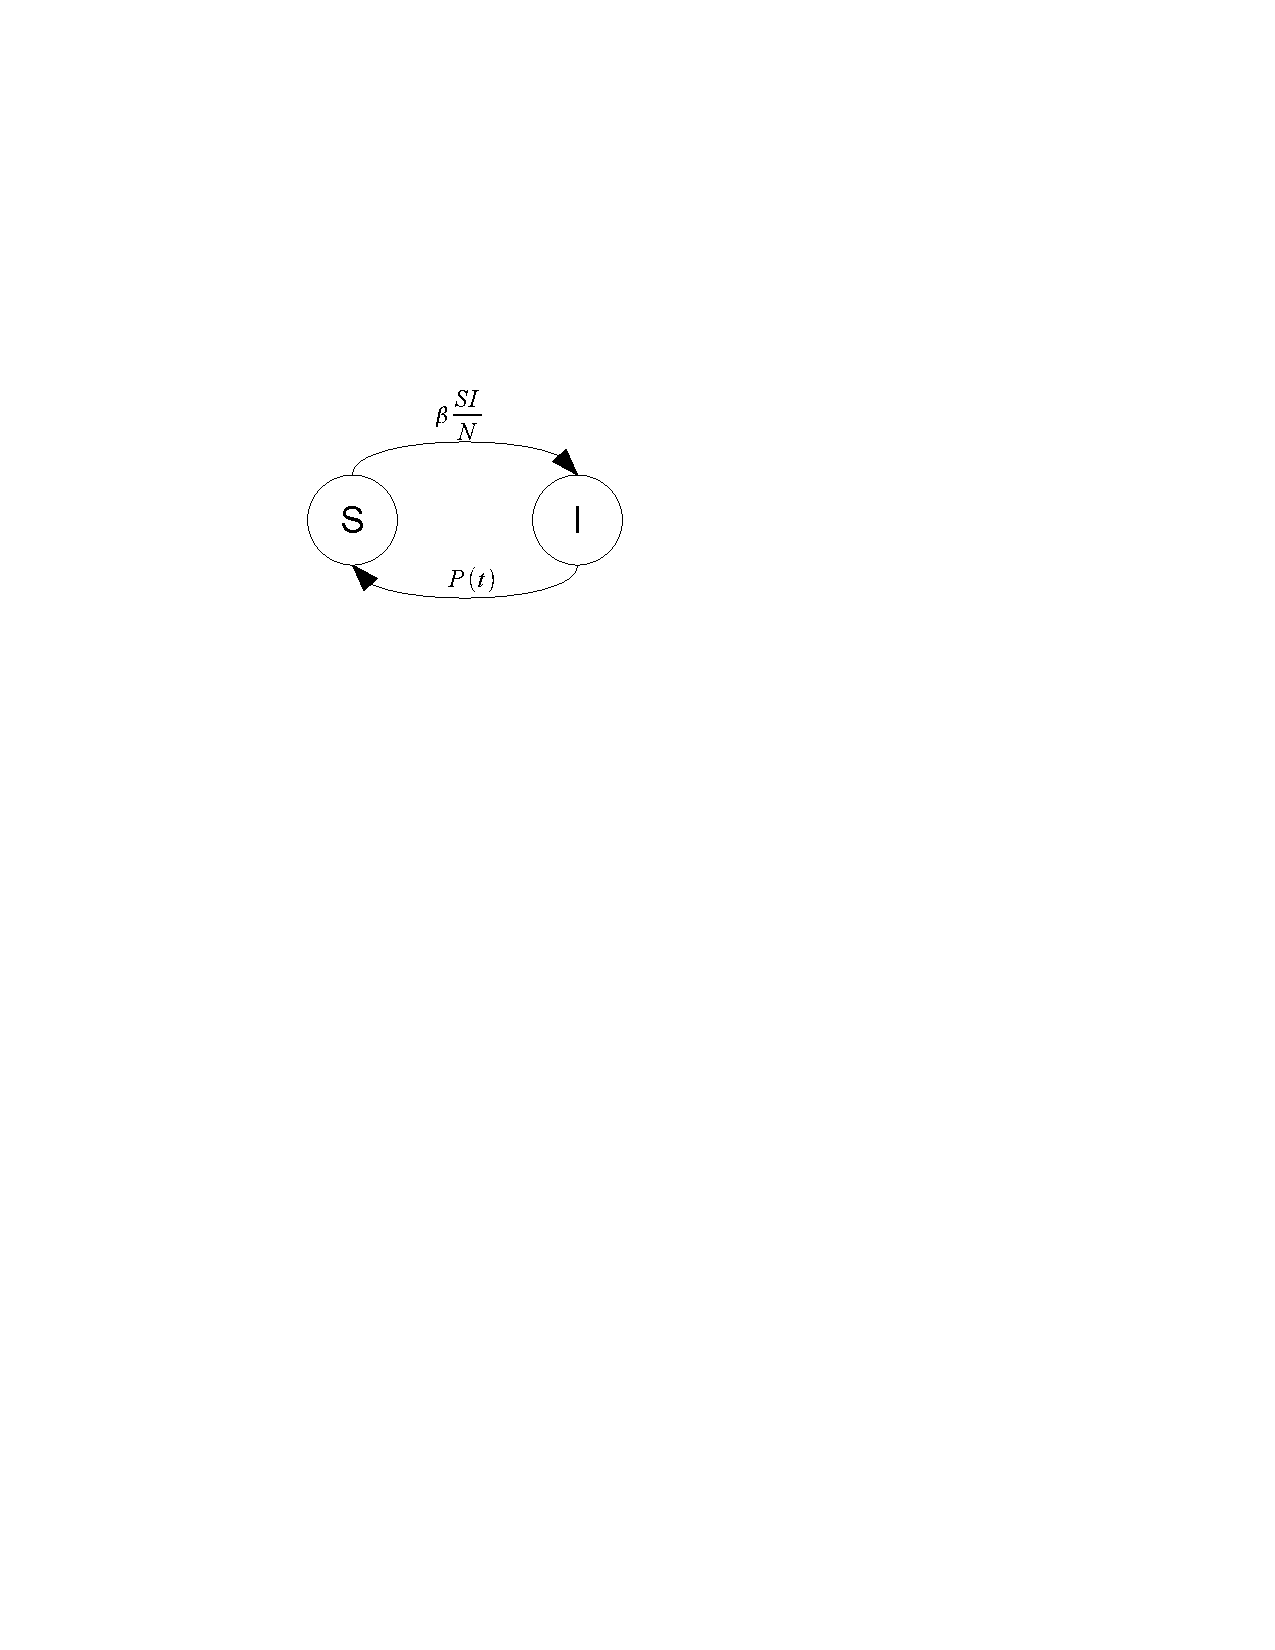
\includegraphics[width=0.5\textwidth]{residence_time/SIS_general}
\end{center}
}


\frame{\frametitle{Reducing the dimension of the problem}
To formulate our model, we would in principle require an equation for $S$ and an equation for $I$.

\vskip1cm
But we have
\[
S(t)+I(t)=N, \textrm{ or equivalently, }S(t)=N-I(t).
\]
$N$ is constant (equal total population at time $t=0$), so we can deduce the value of $S(t)$, once we know $I(t)$, from the equation $S(t)=N-I(t)$.

\vskip1cm
We only need to consider 1 equation. {\bf Do this when possible!} (nonlinear systems are hard, one less equation can make a lot of difference)
}

\frame{\frametitle{Model for infectious individuals}
Integral equation for the number of infective individuals: 
\begin{equation}
I(t) = I_0(t)+ \int_0^t\beta\frac{(N-I(u))I(u)}{N} P(t-u) du
\label{eq:SIS_I} 
\end{equation}
\begin{itemize}
\item $I_0(t)$ number of individuals who were infective at time
$t=0$ and still are at time $t$.
\begin{itemize}
\item $I_0(t)$ is nonnegative, nonincreasing, and
such that $\lim_{t\to\infty}I_0(t)=0$.
\end{itemize}
\item $P(t-u)$ proportion of individuals who became infective at time $u$ and
who still are at time $t$.
\item $\beta (N-I(u))S(u)/N$ is $\beta S(u)I(u)/N$ with $S(u)=N-I(u)$, from the reduction of dimension.
\end{itemize}
}


\frame{\frametitle{Case of an exponentially distributed time to recovery}
Suppose that $P(t)$ is such that the sojourn time in the infective
state has an exponential distribution with mean $1/\gamma$,
\emph{i.e.}, $P(t)=e^{-\gamma t}$.
\vskip0.5cm
Then the initial condition function $I_0(t)$ takes the form
\[
I_0(t)=I_0(0)e^{-\gamma t},
\]
with $I_0(0)$ the number of infective individuals at time $t=0$. This is obtained by considering the cohort of initially infectious individuals, giving a model such as \eqref{eq:N_general}.
\vskip0.5cm
Equation (\ref{eq:SIS_I}) becomes
\begin{equation}\label{eq:I_ODE}
I(t)=I_0(0)e^{-\gamma t}+\int_0^t \beta\frac{(N-I(u))I(u)}{N} e^{-\gamma (t-u)}du.
\end{equation}
}

\frame{
Taking the time derivative of \eqref{eq:I_ODE} yields
\begin{align*}
I'(t) &= \beta \frac{(N-I(t))I(t)}{N}-\gamma I(t),
\end{align*}
which is the classical logistic type ordinary differential equation
(ODE) for $I$ in an SIS model without vital dynamics (no birth or death).
}

\frame{\frametitle{Conclusion}
\begin{itemize}
\item The time of sojourn in classes (compartments) plays an important role in determining the type of model that we deal with.
\item All ODE models, when they use terms of the form $\kappa X$, make the assumption that the time of sojourn in compartments is exponentially distributed.
\item At the other end of the spectrum, delay delay differential with discrete delay make the assumption of a constant sojourn time, equal for all individuals.
\end{itemize}
\vskip1cm
\begin{itemize}
\item Both can be true sometimes.. but reality is often somewhere in between.
\end{itemize}
}


%%%%%%%%%%%%%%
%%%%%%%%%%%%%%
%%%%%%%%%%%%%%
%%%%%%%%%%%%%%
\section{Epidemic models}

\subsection{SIS model without vital dynamics}


\frame{\frametitle{A SIS model}
Consider a disease that confers no immunity. In this case,
individuals are either
\begin{itemize}
\item \emph{susceptible} to the disease, with the number of such individuals at time $t$ denoted by $S(t)$,
\item or \emph{infected} by the disease (and are also \emph{infective} in the sense that they propagate the disease), with the number of such individuals at time $t$ denoted by $I(t)$.
\end{itemize}
\vskip1cm
We want to model the evolution with time of $S$ and $I$ ($t$ is omitted unless necessary).
}

\frame{\frametitle{Hypotheses}
\begin{itemize}
\item Individuals recover from the disease at the \emph{per capita} rate $\gamma$.
\item The disease does not confer immunity.
\item There is no birth or death.
\item Infection is of \emph{standard incidence} type, $\beta=SI/N$.
\end{itemize}
}


\frame{\frametitle{Flow diagram of the model}
\begin{center}
    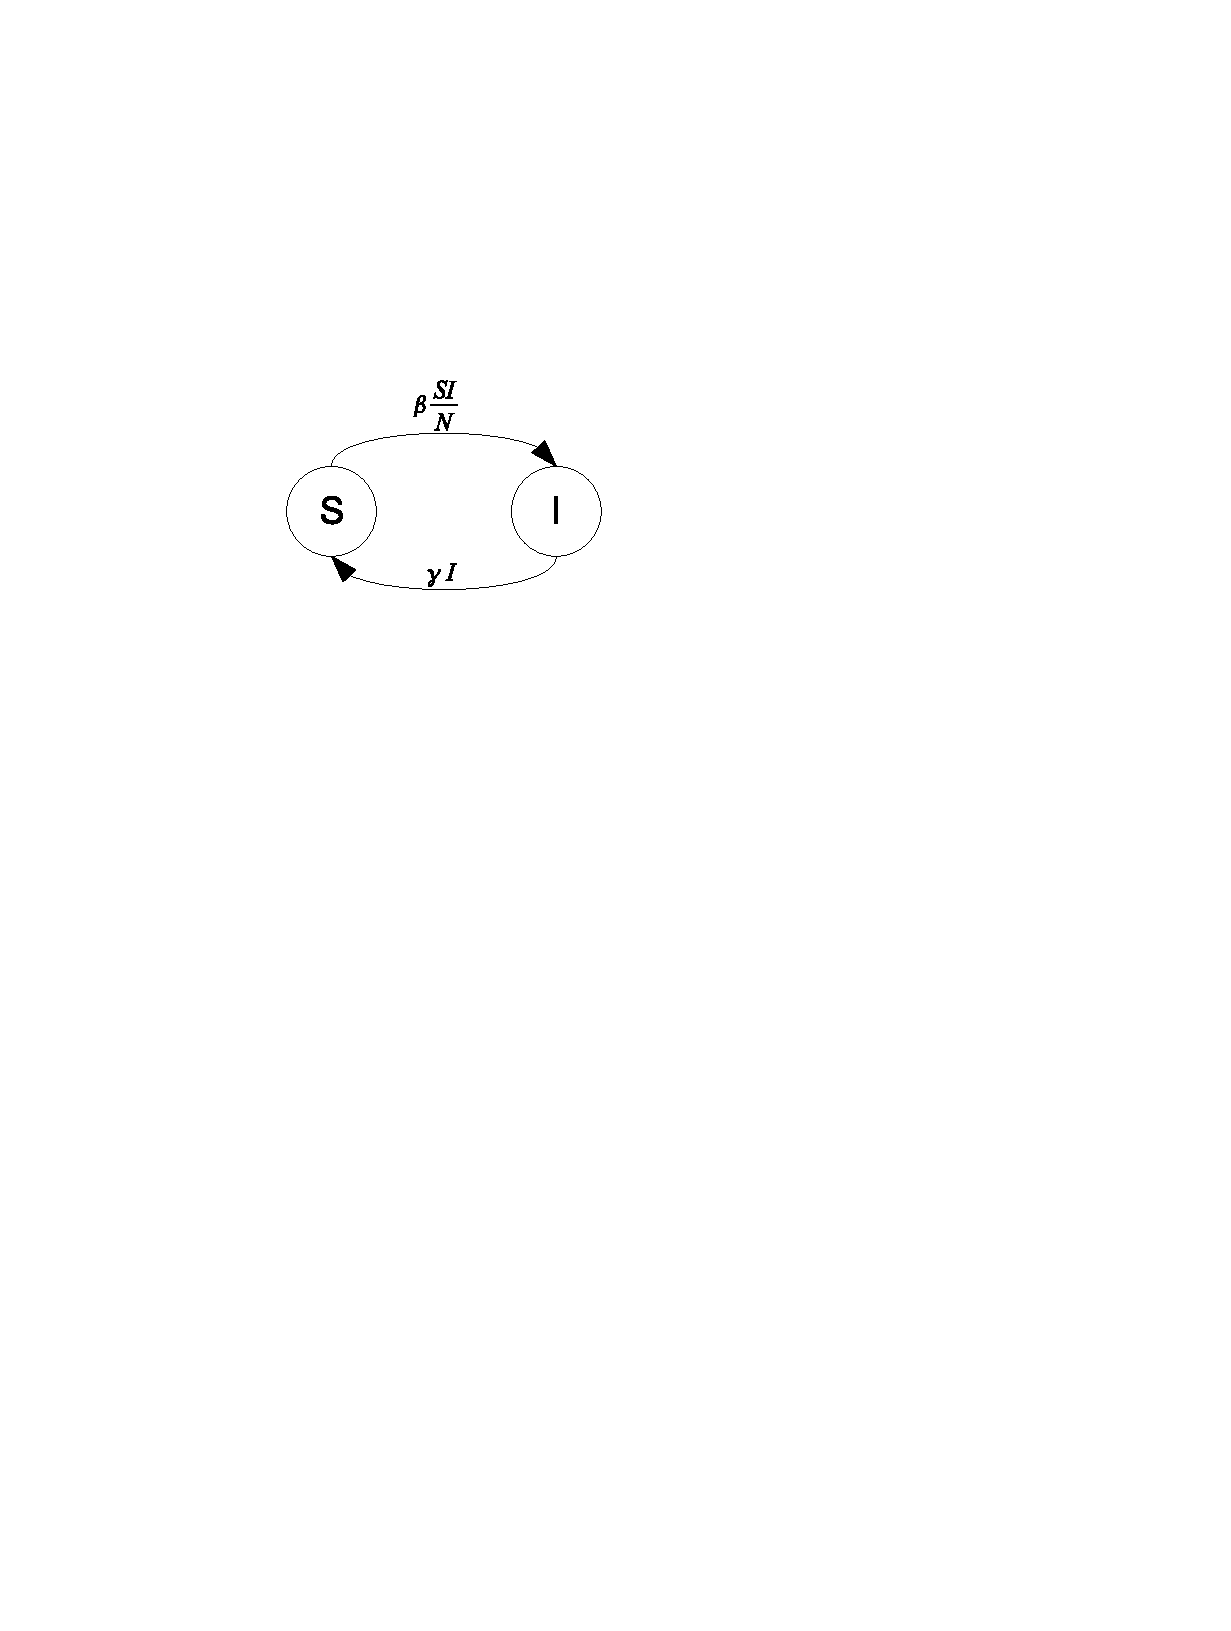
\includegraphics[width=0.5\textwidth]{epidemic_models/SIS_nodemography}
\end{center}
}


\frame{
The evolution of $I(t)$ is described by the following equation (see slides on \emph{residence time}):
\[
I'= \beta \frac{(N-I)I}{N}-\gamma I.
\]
Develop and reorder the terms, giving
\begin{equation}\label{sys:I_nodemography}
I'=(\beta-\gamma)I-\frac{\beta}{N} I^2
\end{equation}
}

\frame{\frametitle{The basic reproduction number}
Define the \emph{basic reproduction number} (the average number of people that an infectious individual will infect, when introduced in a population of susceptibles) as 
\[
\Rzero=\frac\beta\gamma
\]
We have
\[
\left(\Rzero<1\Leftrightarrow (\beta-\gamma)<0\right)\textrm{ and }\left(\Rzero>1\Leftrightarrow (\beta-\gamma)>0\right).
\]
Then
\begin{itemize}
\item If $\Rzero<1$, then $\lim_{t\to\infty}I(t)=0$.
\item If $\Rzero>1$, then
\[
lim_{t\to\infty} I(t)=\left(1-\frac{1}{\Rzero}\right)N.
\]
\end{itemize}
(the case $\Rzero=1$ is usually omitted)
}

\frame{
\begin{center}
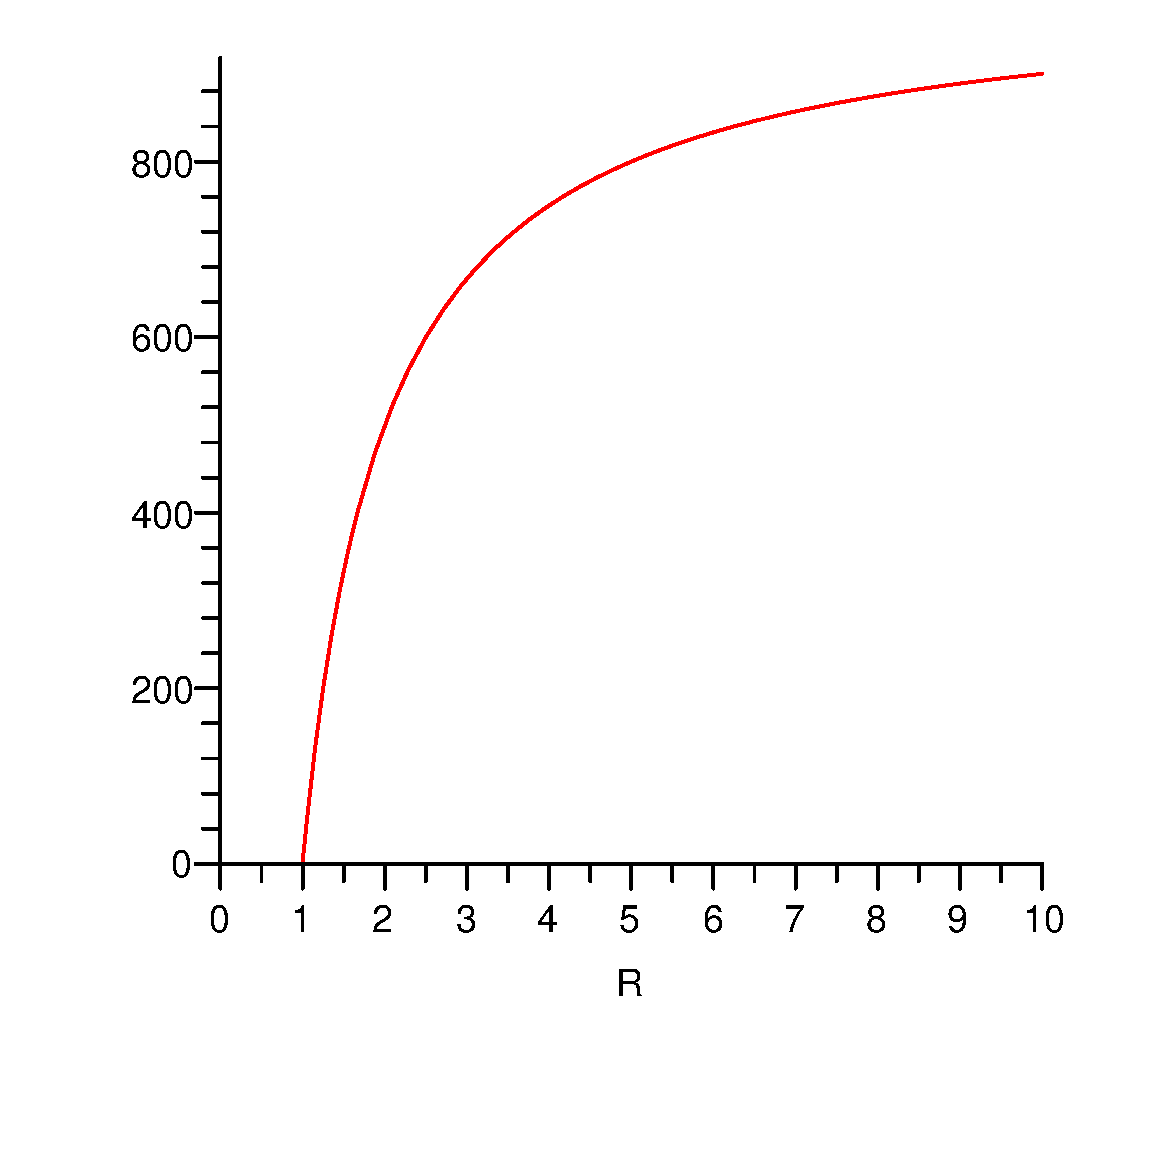
\includegraphics[width=0.6\textwidth]{epidemic_models/EEP_fct_R0}
\end{center}
}


\subsection{SIR model of Kermack and McKendrick}

\frame{\frametitle{Kermack and McKendrick}
In 1927, Kermack and McKendrick started publishing a series of papers on epidemic models. In the first of their papers, they have this model as a particular case:
\begin{equation}\label{sys:KMK}
\begin{aligned}
S' &= -\beta SI \\
I' &= \beta SI-\gamma I \\
R' &= \gamma I
\end{aligned}
\end{equation}
}

\frame{\frametitle{Analyzing the system}
First, note (as KMK) that the total population in the system is constant. This is deduced from the fact that
\[
N'=(S+I+R)'=-\beta SI+\beta SI-\gamma I+\gamma I=0.
\]
Since this is true for all values of $t$, we have $N$ constant.
}

\frame{
Let us ignore the $R$ equation for now.
We can compute
\[
\frac{dI}{dS}=\frac{dI}{dt}\frac{dt}{dS}=\frac{I'}{S'}=\frac{\gamma}{\beta S}-1
\]
This gives
\[
I(S)=S-\frac{\gamma}{\beta}\ln S+K,
\]
which, considering the initial condition $(S_0,I_0)$, is,
\[
I(S)=S-\frac{\gamma}{\beta}\ln S+I_0-(S_0-\frac{\gamma}{\beta}\ln S_0).
\]
This gives a curve in the $(S,I)$ plane.
}


\frame{
\[
I(S)=S-\frac{\gamma}{\beta}\ln S+I_0-(S_0-\frac{\gamma}{\beta}\ln S_0).
\]
Typically, assume $S\approx N$ and $I>0$ small.
Let us denote $S_\infty=\lim_{t\to\infty}S(t)$.

We want to find the value of $S$ when $I\to 0$.
Then
\[
I_0-\frac\gamma\beta\ln S_0=S_\infty -\frac\gamma\beta \ln S_\infty
\]
}

\subsection{SIRS model with demography}

\frame{\frametitle{The SIRS model -- Assumptions (1/2)}
\begin{itemize}
\item Like KMK, individuals are S, I or R.
\item Infection is $\beta SI$ (mass action) or $\beta SI/N$ (proportional incidence).
\item Different interpretation of the R class: R stands for ``removed'', individuals who are immune to the disease following recovery.
\item Recovery from the disease (movement from I class to R class) occurs at the per capita rate $\gamma$.\\ (Time spent in I before recovery is exponentially distributed.)
\item Immunity can be lost: after some time, R individuals revert back to S individuals.
\item Time spent in R class before loss of immunity is exponentially distributed, with mean $1/\nu$.
\end{itemize}
}

\frame{\frametitle{The SIRS model -- Assumptions (2/2)}
\begin{itemize}
\item There is birth and death of individuals:
\begin{itemize}
\item No vertical transmission of the disease (mother to child) or of immunity, so all birth is into the S class.\\ Birth occurs at the rate $\Pi$.
\item Individuals in all classes die of at the per capita rate $d$, i.e., the average life duration is exponentially distributed with mean $1/d$.
\item The disease is lethal: infected individuals are subject to additional mortality at the per capita rate $\delta$.
\end{itemize}
\end{itemize}
Note that birth and death can have different interpretations:
\begin{itemize}
\item birth and death in the classical sense,
\item but also, entering the susceptible population and leaving it.
\end{itemize}
}

\frame{\frametitle{Flow diagrams for the models}
\begin{description}
\item[Mass action]\qquad
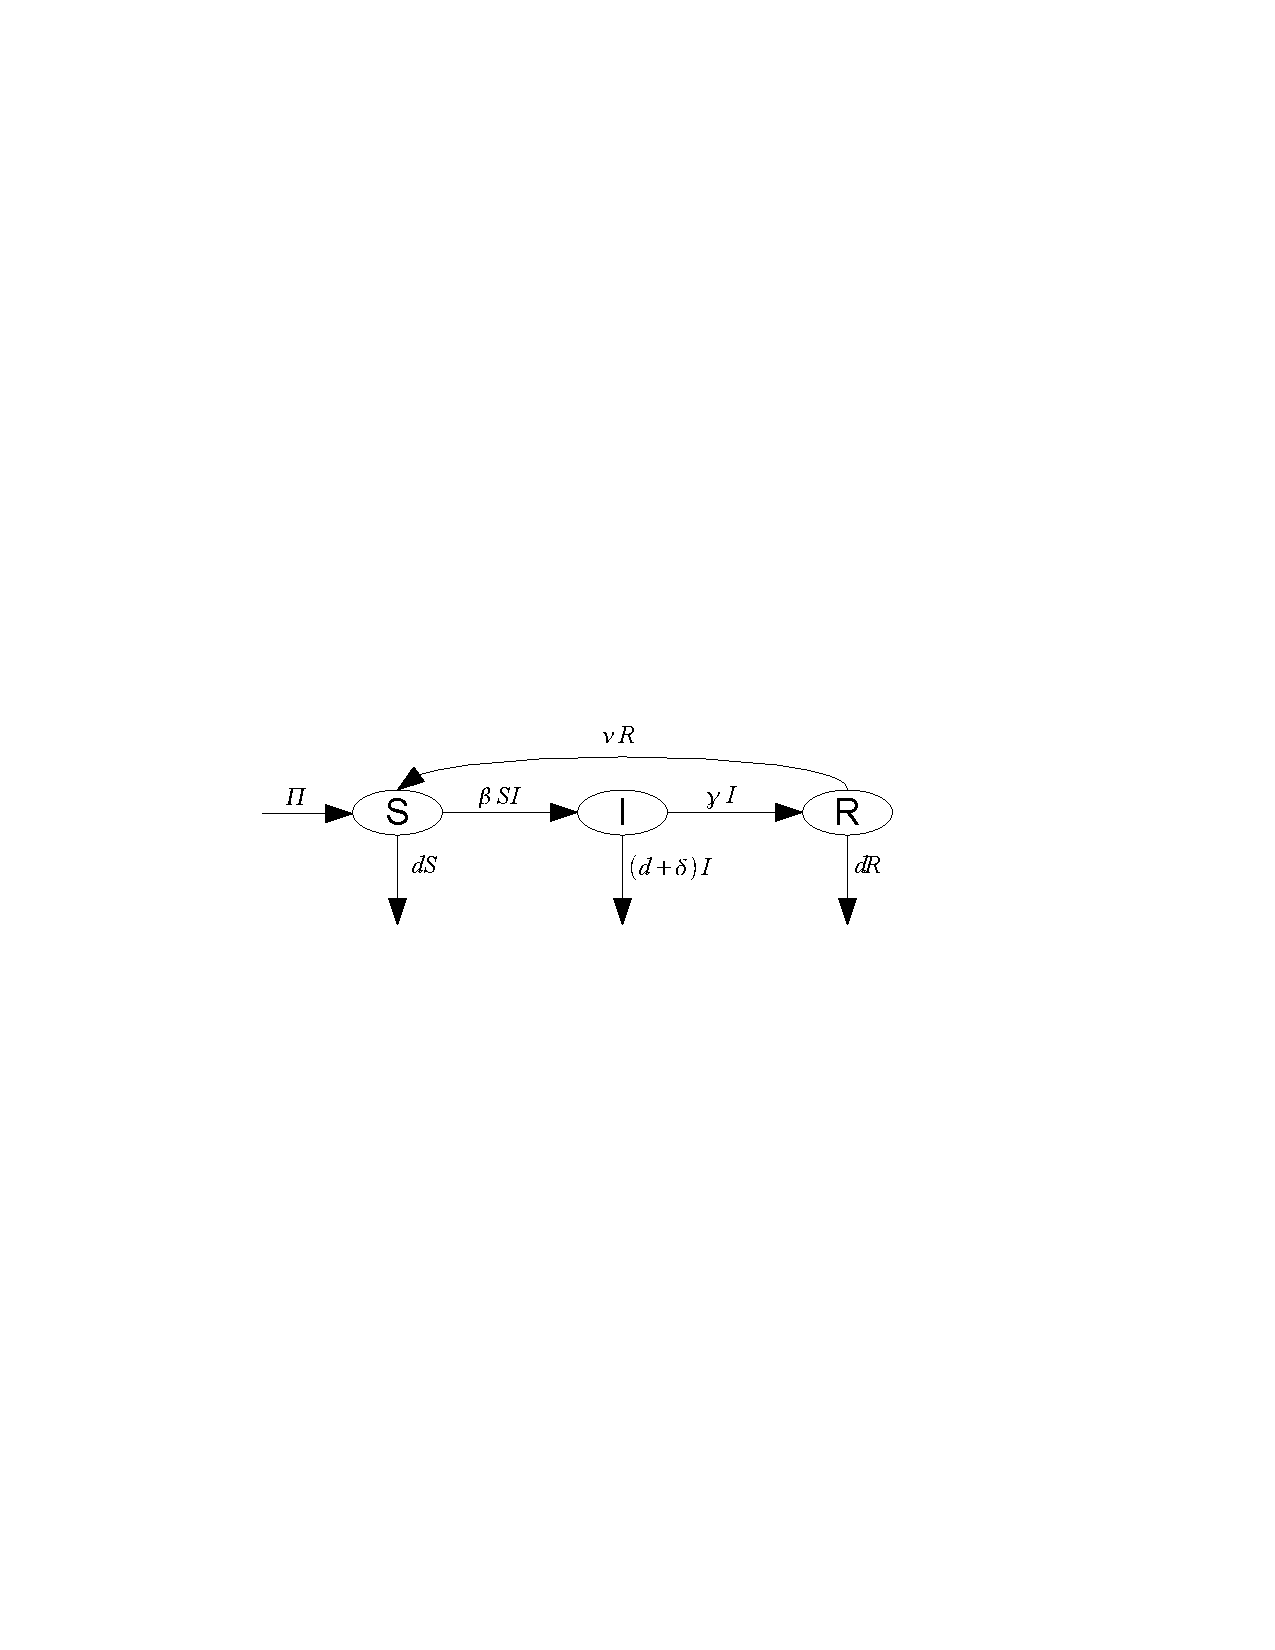
\includegraphics[width=0.75\textwidth]{epidemic_models/SIRS_massaction}\vskip1cm
\item[Standard incidence]
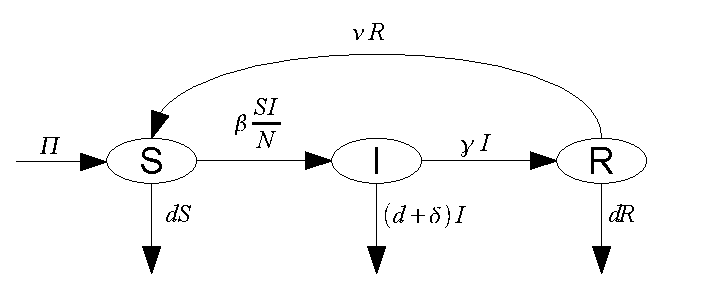
\includegraphics[width=0.75\textwidth]{epidemic_models/SIRS_propincidence}
\end{description}
}

\frame{\frametitle{SIRS model with mass action incidence}
Consider the model with mass action incidence,
\begin{align*}
S' &= \Pi+\nu R-\beta SI-dS \\
I' &= \beta SI-(d+\delta+\gamma)I \\
R' &= \gamma I-(d+\nu)R
\end{align*}
}




%%%%%%%%%%%%%%
%%%%%%%%%%%%%%
%%%%%%%%%%%%%%
%%%%%%%%%%%%%%
\section{The chemostat}

\frame{\frametitle{A chemostat}
\begin{center}
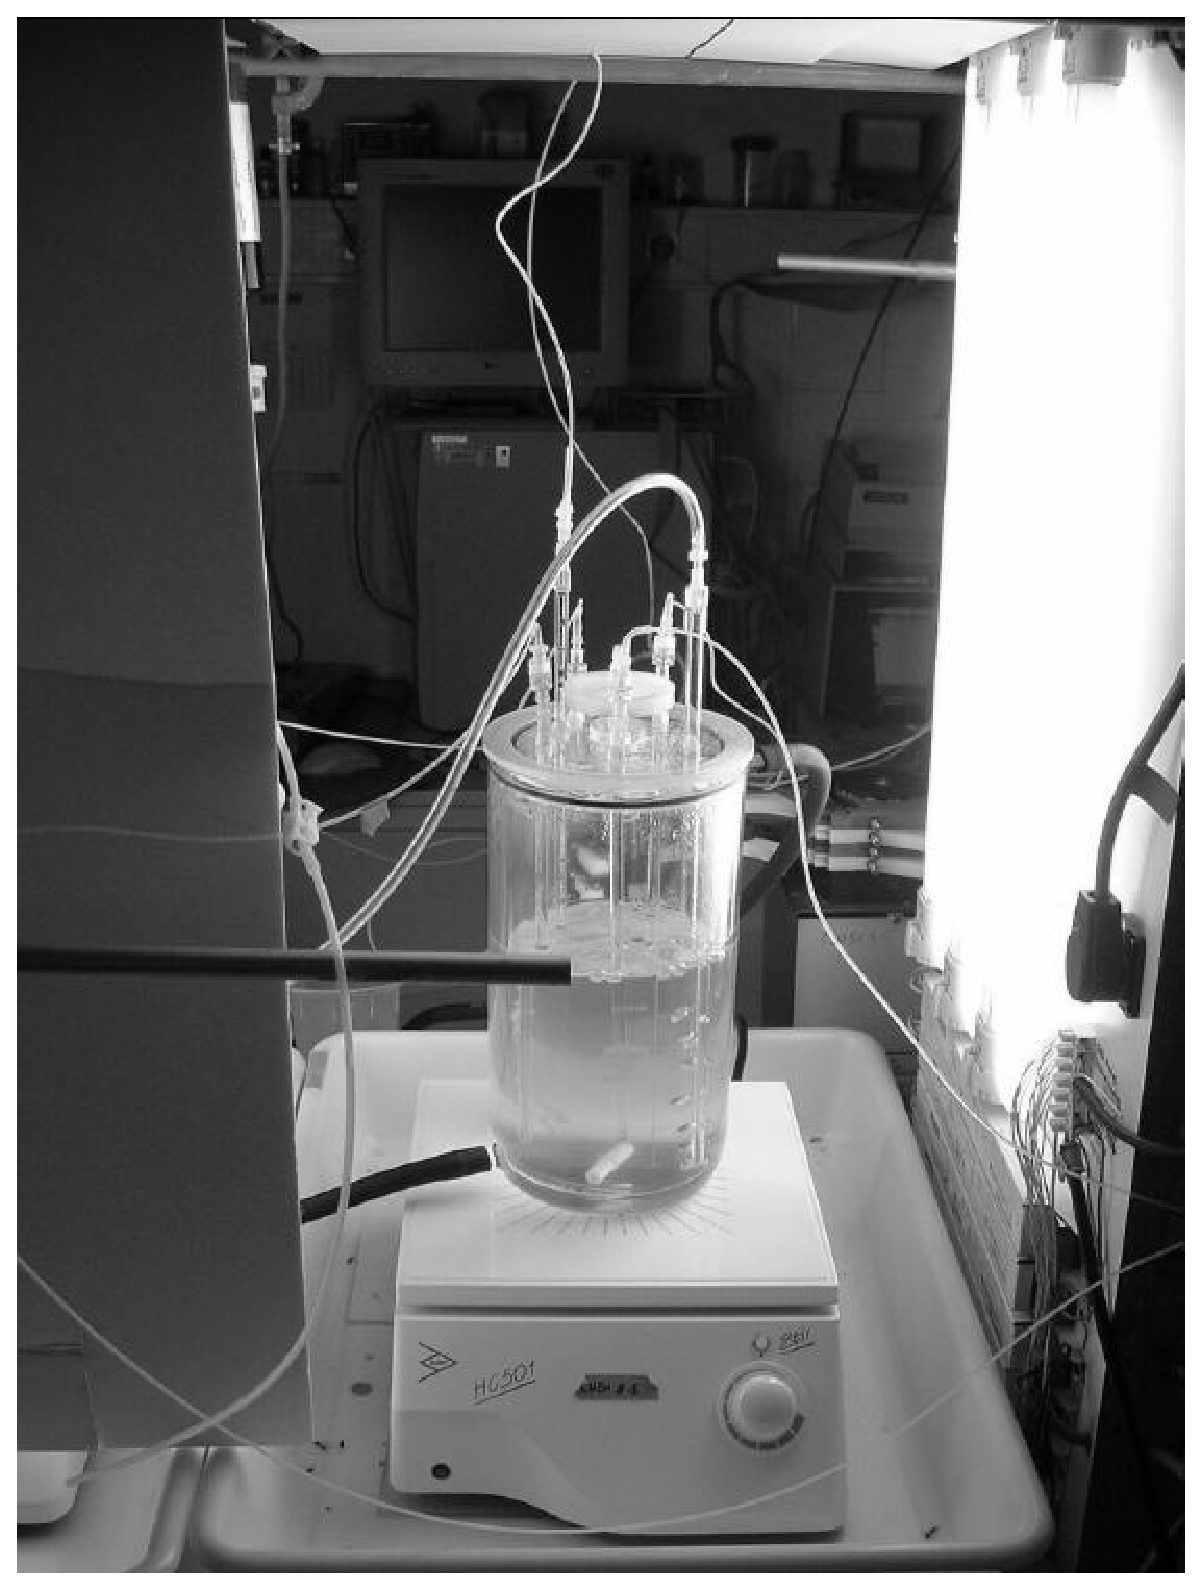
\includegraphics[height=0.9\textheight]{chemostat/chemostat}
\end{center}
}

\frame{\frametitle{Principle}
\begin{itemize}
\item
One main chamber (vessel), in which some microorganisms (bacteria, plankton), typically unicellular, are put, together with liquid and nutrient.
\item
Contents are stirred, so nutrient and organisms are well-mixed.
\item
Organisms consume nutrient, grow, multiply.
\item
Two major modes of operation:
\begin{itemize}
\item \emph{Batch} mode: let the whole thing sit.
\item \emph{Continuous flow} mode: there is an input of fresh water and nutrient, and an outflow the comprises water, nutrient and organisms, to keep the volume constant.
\end{itemize}
\end{itemize}
}


\subsection{Batch mode}


\frame{\frametitle{Model for batch mode -- No organism death}
First, assume no death of organisms. Model is
\begin{subequations}\label{sys:chemo_batch_nodeath}
\begin{align}
S' &= -\mu(S)x \\
x' &= \mu(S)x
\end{align}
\end{subequations}
with initial conditions $S(0)\geq 0$ and $x(0)>0$, and
where $\mu(S)$ is such that
\begin{itemize}
\item $\mu(0)=0$ (no substrate, no growth)
\item $\mu(S)\geq 0$ for all $S\geq 0$
\item $\mu(S)$ bounded for $S\geq 0$
\end{itemize}
}


\frame{\frametitle{The Michaelis-Menten curve}
Typical form for $\mu(S)$ is the \emph{Michaelis-Menten} (MM) curve,
\begin{equation}\label{eq:monod}
\mu(S)=\mu_{max}\frac S{K_S+S}
\end{equation}
\begin{minipage}[b]{0.5\textwidth}
\begin{itemize}
\item $\mu_{max}$ maximal growth rate
\item $K_S$ half-saturation constant ($\mu(K_S)=\mu_{max}/2$).
\end{itemize}
\end{minipage}
\begin{minipage}{0.45\textwidth}
\begin{center}
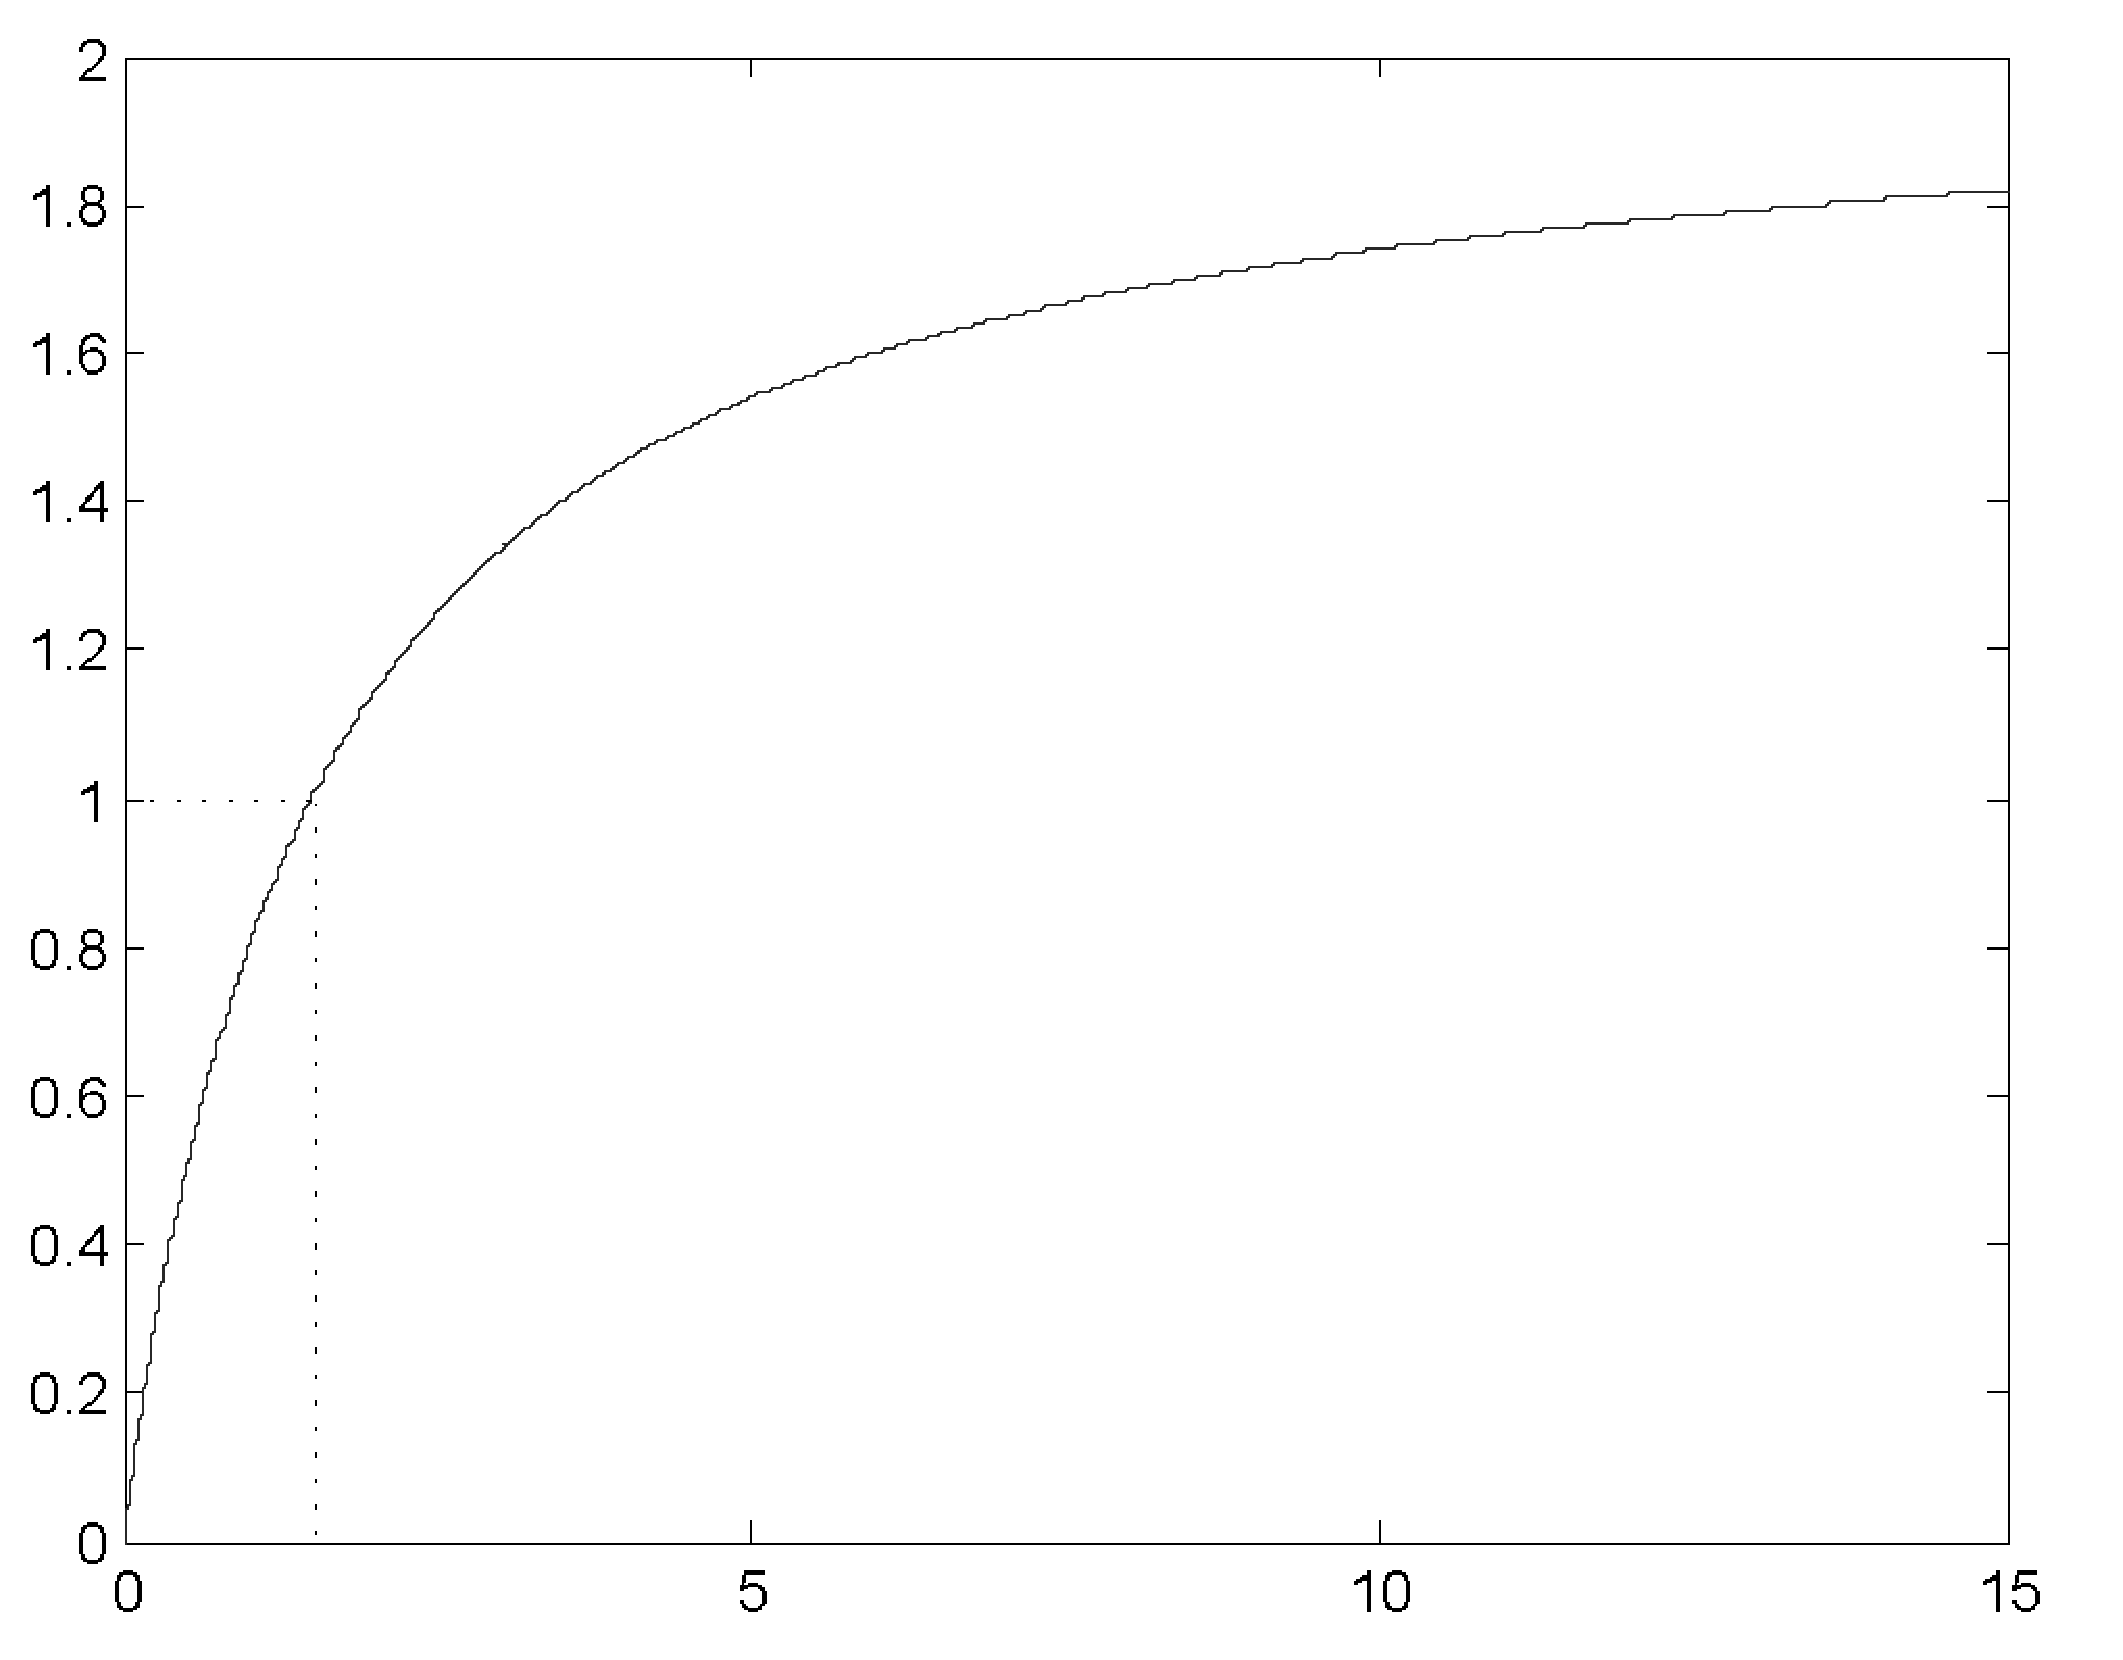
\includegraphics[width=\textwidth]{chemostat/monod}
\end{center}
\end{minipage}
From now on, assume MM function.
}


\frame{\frametitle{Equilibria}
To compute the equilibria, suppose $S'=x'=0$, giving
\[
\mu(S)x=-\mu(S)x=0
\]
This implies $\mu(S)=0$ or $x=0$. Note that $\mu(S)=0\Leftrightarrow S=0$, so the system is at equilibrium if $S=0$ or $x=0$.

\vskip1cm
This is a complicated situation, as it implies that there are lines of equilibria ($S=0$ and any $x$, and $x=0$ and any $S$), so that the equilibria are not \emph{isolated} (arbitrarily small neighborhoods of one equilibrium contain other equilibria), and therefore, studying the linearization is not possible.
}

\frame{
Here, some analysis is however possible.
Consider
\[
\frac{dx}{dS}=\frac{dx}{dt}\frac{dt}{dS}=-\frac{\mu(S)x}{\mu(S)x}=-1
\]
This implies that we can find the solution
\[
x(S)=C-S,
\]
or, supposing the initial condition is $(S(0),x(0))=(S_0,x_0)$, that is, $x(S_0)=x_0$,
\[
x(S)=S_0+x_0-S
\]
\begin{center}
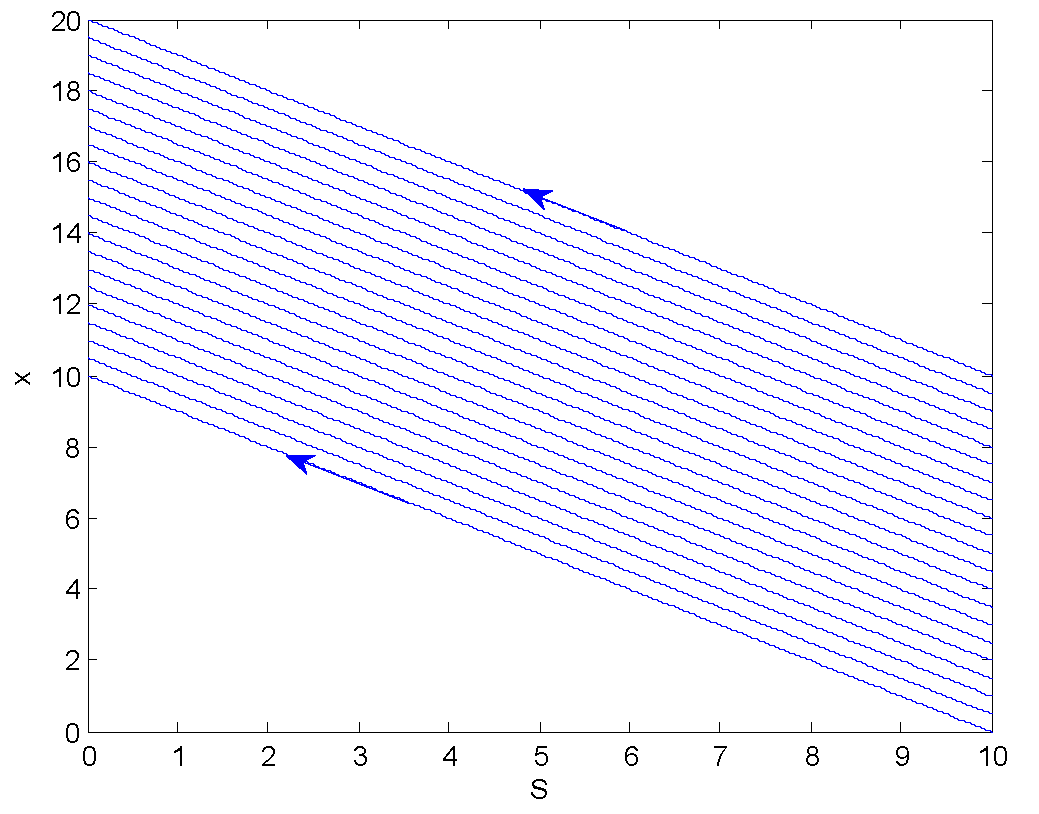
\includegraphics[width=0.5\textwidth]{chemostat/chemo_batch_nodeath_Sx}
\end{center}
}


\frame{\frametitle{Model for batch mode -- Organism death}
Assume death of organisms at per capita rate $d$. Model is
\begin{subequations}\label{sys:chemo_batch_death}
\begin{align}
S' &= -\mu(S)x \\
x' &= \mu(S)x-dx
\end{align}
\end{subequations}
}


\frame{\frametitle{Equilibria}
$S'=0\Leftrightarrow \mu(S)x=0$

$x'=0\Leftrightarrow (\mu(S)-d)x=0$.

So we have $x=0$ or $\mu(S)=d$. So $x=0$ and any value of $S$, and $S$ such that $\mu(S)=d$ and $x=0$. One such particular value is $(S,x)=(0,0)$.

\vskip1cm
This is once again a complicated situation, since there are lines of equilibria. Intuitively, most solutions will go to $(0,0)$. This is indeed the case (we will not show it).
}


\subsection{Continous flow mode}


\frame{\frametitle{Modelling principles -- Continuous flow mode}
\begin{itemize}
\item Organisms (concentration denoted $x$) are in the main vessel.
\item Limiting substrate (concentration in the vessel denoted $S$) is input (at rate $D$ and concentration $S^0$).
\item There is an outflow of both nutrient and organisms (at same rate $D$ as input). 
\item Homogeneous mixing.
\item Residence time in device is assumed small compared to lifetime (or time to division) $\Rightarrow$ no death considered.
\end{itemize}
}

\frame{\frametitle{Schematic representation}
\begin{center}
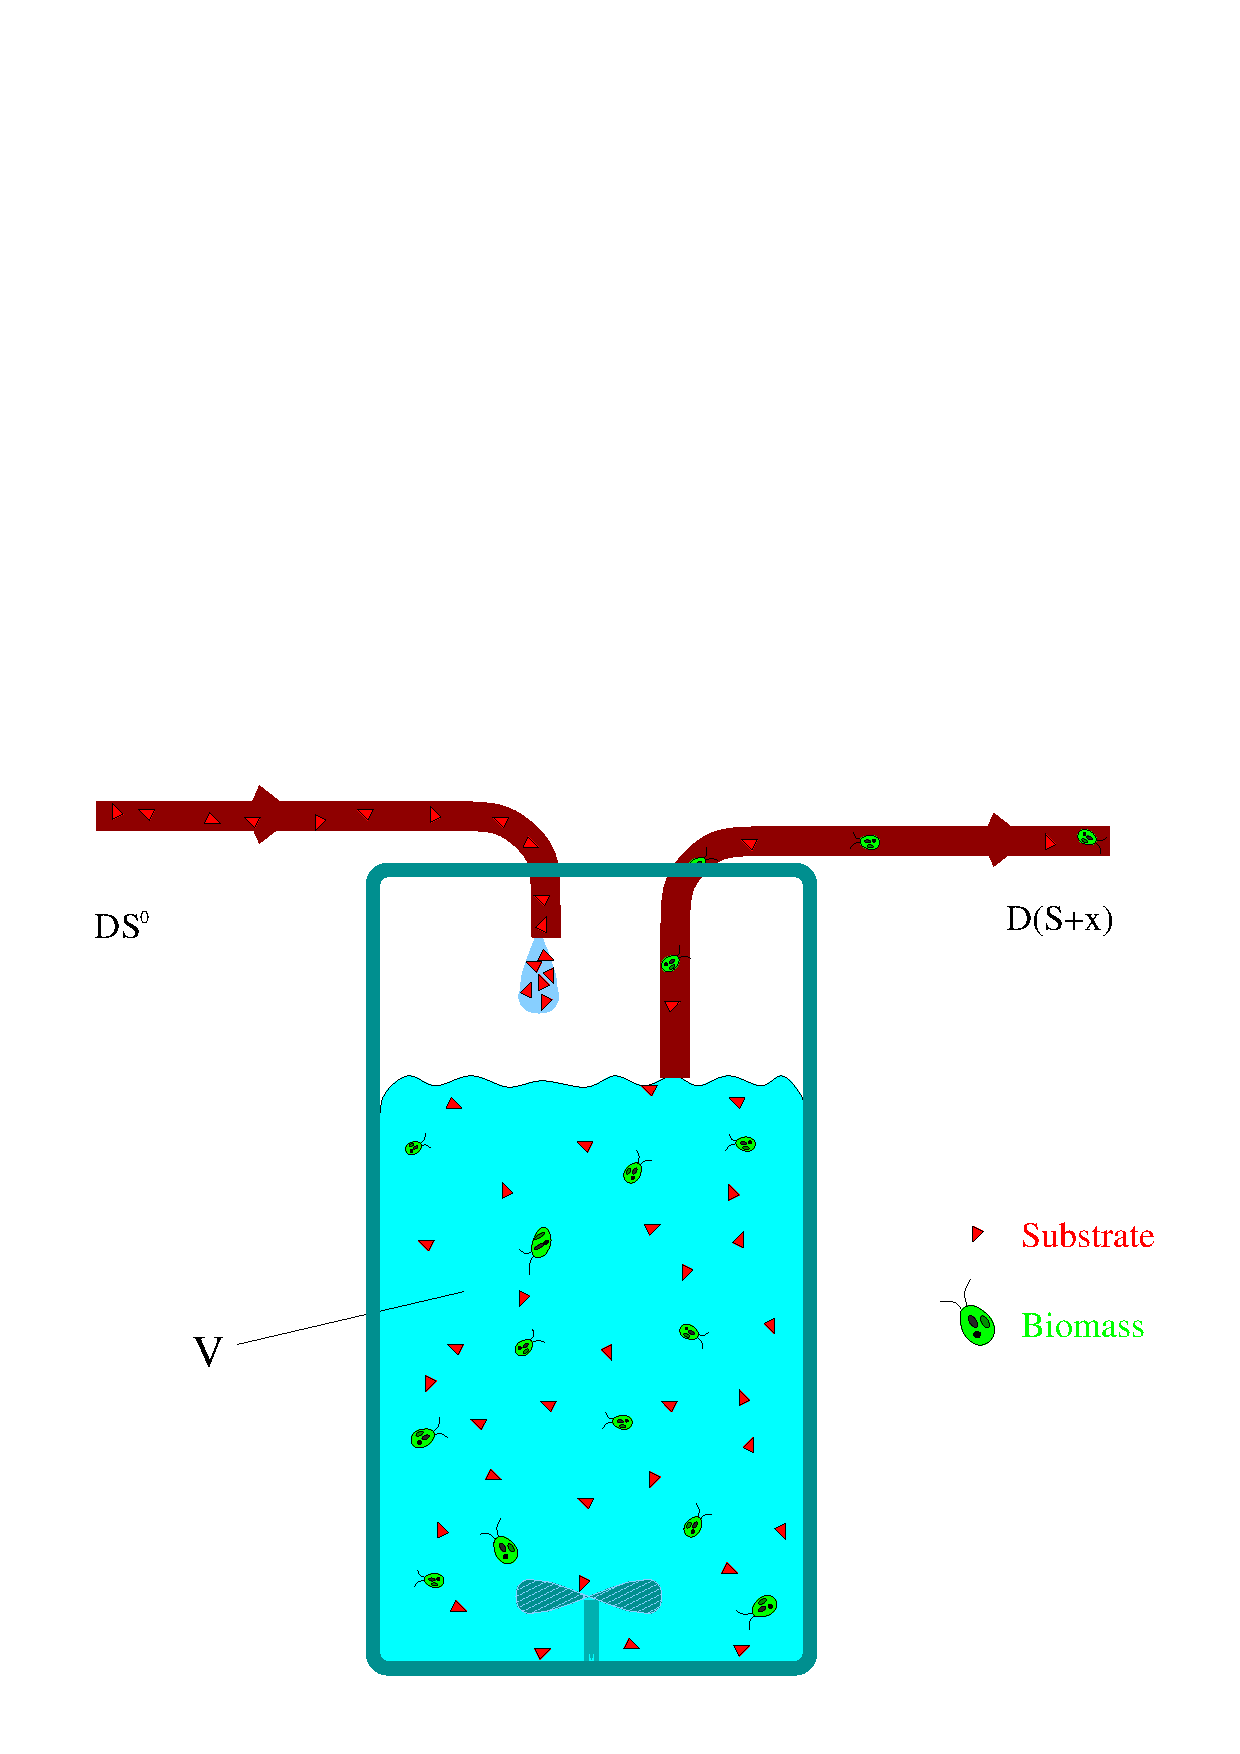
\includegraphics[height=0.9\textheight]{chemostat/figchemo_eng}
\end{center}
}

\frame{\frametitle{Model for continuous flow mode}
Model is
\begin{subequations}\label{sys:chemo_flow}
\begin{align}
S' &= D(S^0-S)-\mu(S)x \\
x' &= \mu(S)x-Dx
\end{align}
\end{subequations}
with initial conditions $S(0)\geq 0$ and $x(0)\geq 0$, and $D,S^0>0$.
}


\frame{\frametitle{Equilibria}
Existence: done in class using nullclines.
\vskip1cm
Stability: done in class using Jacobian matrix.
}




%%%%%%%%%%%%%%
%%%%%%%%%%%%%%
%%%%%%%%%%%%%%
%%%%%%%%%%%%%%
\section{Traffic flow}

\subsection{ODE model}

\frame{\frametitle{Hypotheses}
\begin{itemize}
\item $N$ cars in total.
\item Road is the $x$-axis.
\item $x_n(t)$ position of the $n$th car at time $t$.
\item $v_n(t)\stackrel{\Delta}{=}x_n'(t)$ velocity of the $n$th car at time $t$.
\end{itemize}
\begin{center}
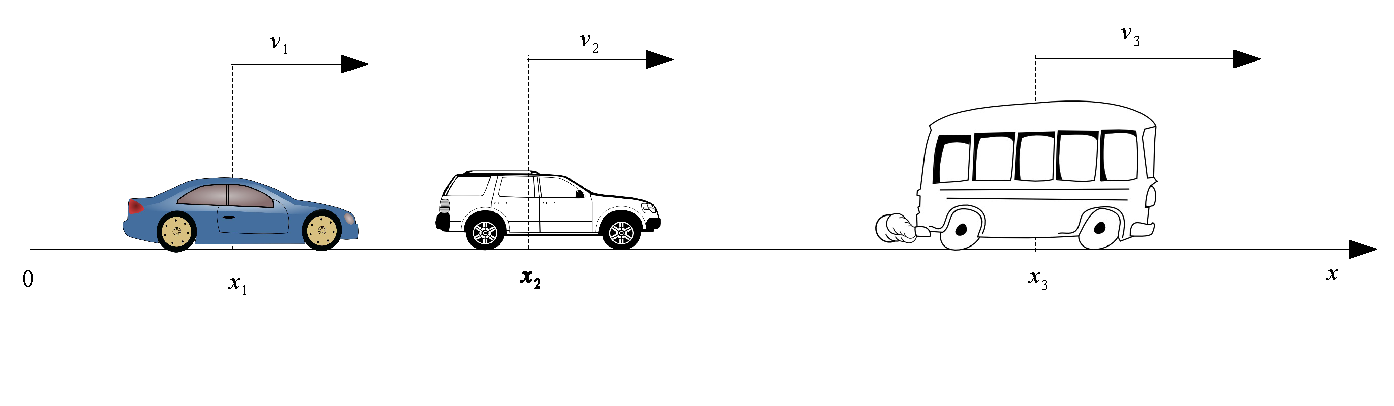
\includegraphics[width=\textwidth]{traffic_flow/traffic_flow1}
\end{center}
\begin{itemize}
\item All cars start with the same initial speed $v_0$ before time $t=0$.
\end{itemize}
}

\frame{\frametitle{Moving frame coordinates}
To make computations easier, express velocity of cars in a reference frame moving at speed $u_0$.
\vskip1cm
Remark that here, speed=velocity, since movement is 1-dimensional.
\vskip1cm
Let
\[
u_n(t)=v_n(t)-u_0.
\]
Then $u_n(t)=0$ for $t\leq 0$, and $u_n$ is the speed of the $n$th car in the moving frame coordinates.
}

\frame{\frametitle{Modeling driver behavior}
Assume that
\begin{itemize}
\item Driver adjusts his/her speed according to relative speed between his/her car and the car in front.
\item This adjustment is a linear term, equal to $\lambda$ for all drivers.
\end{itemize}
\vskip1cm
\begin{itemize}
\item
First car: evolution of speed remains to be determined.
\item 
Second car:
\[
u_2'=\lambda(u_1-u_2).
\]
\item
Third car:
\[
u_3'=\lambda(u_2-u_3)
\]
\item 
Thus, for $n=1,\ldots,N-1$,
\begin{equation}\label{eq:ode}
u_{n+1}'=\lambda(u_n-u_{n+1}).
\end{equation}
\end{itemize}
}


\frame{
This can be solved using \emph{linear cascades}: if $u_1(t)$ is known, then
\[
u_2'=\lambda(u_1(t)-u_2)
\]
is a linear first-order nonhomogeneous equation. Solution (integrating factors, or variation of constants) is
\[
u_2(t)=\lambda e^{-\lambda t}\int_0^t u_1(s)e^{\lambda s}ds
\]
Then use this function $u_2(t)$ in $u_3'$ to get $u_3(t)$,
\begin{align*}
u_3(t) &= \lambda e^{-\lambda t}\int_0^t u_2(s)e^{\lambda s}ds
\end{align*}
}

\frame{\frametitle{Example}
Suppose driver of car 1 follows this function
\[
u_1(t)=\alpha\sin(\omega t)
\]
that is, $\omega$-periodic, 0 at $t=0$ (we want all cars to start with speed relative to the moving reference equal to 0), and with amplitude $\alpha$.

\vskip0.5cm
Then
\begin{align*}
u_2(t) &= \frac{\lambda\alpha}{\lambda^2+\omega^2}\left(\omega e^{-\lambda t}
+\lambda\sin(\omega t)-\omega\cos(\omega t)\right).
\end{align*}
When $t\to\infty$, first term goes to 0, we are left with a $\omega$-periodic
term.
}


\frame{\frametitle{Using the theory of linear systems}
Consider the case of 3 cars. Let
\[
X=\begin{pmatrix}
u_2\\ u_3
\end{pmatrix}
\]
Then the system can be written as
\[
X'=\begin{pmatrix}
-\lambda & 0 \\
\lambda & -\lambda
\end{pmatrix}U
+\begin{pmatrix}
\lambda u_1(t)\\ 0
\end{pmatrix}
\]
which we write for short as $X'=AX+B(t)$.
}

\frame{
The matrix $A$ has the eigenvalue $-\lambda$ with multiplicity 2. Its Jordan form is
\[
J=\begin{pmatrix}
-\lambda & 1 \\
0 & -\lambda
\end{pmatrix}
\]
with matrix of change of basis
\[
P=\begin{pmatrix}
0 & 1 \\
\lambda & 0
\end{pmatrix}
\]
which is such that $P^{-1}AP=J$.
}

\frame{
Because $-\lambda$ is an eigenvalue with multiplicity 2 (same as the size of the matrix), we can use the simplified theorem, and only need $N$. 
\vskip1cm
We have
\begin{align*}
N &= A-S \\
&=\begin{pmatrix}
-\lambda & 0 \\
\lambda & -\lambda
\end{pmatrix}
-
\begin{pmatrix}
-\lambda & 0 \\
0 & -\lambda
\end{pmatrix} \\
&=\begin{pmatrix}
0 & 0 \\
\lambda & 0
\end{pmatrix}
\end{align*}
}


\frame{
Clearly, $N^2=0$, so, by the theorem in the simplified case,
\begin{align*}
x(t) &= e^{-\lambda t}\left(\II+Nt\right)x_0 \\
\end{align*}
But we know that solutions are unique, and that the solution to the differential equation is given by $x(t)=e^{At}x_0$. This means that
\begin{align*}
e^{At} &= e^{-\lambda t}\left(\II+Nt\right)\\
&= e^{-\lambda t}\left(\begin{pmatrix}1&0\\0&1\end{pmatrix}+
\begin{pmatrix}
0 & 0 \\
\lambda t & 0
\end{pmatrix}\right)\\
&= e^{-\lambda t}\begin{pmatrix}
1 & 0 \\
\lambda t & 1
\end{pmatrix} \\
&= \begin{pmatrix}
e^{-\lambda t} & 0 \\
\lambda te^{-\lambda t} & e^{-\lambda t}
\end{pmatrix}
\end{align*}
}

\frame{Now notice that the solution to
\[
X'=AX
\]
is trivially established here, since
\[
X(0)=\begin{pmatrix}u_2(0)\\u_3(0)\end{pmatrix}=\begin{pmatrix}0\\0\end{pmatrix},
\]
and thus
\[
X(t)=e^{At}0=0.
\]
$e^{At}$ does however play a role in the solution (fortunately), since it is involved in the variation of constants formula:
\[
X(t)=e^{At}X_0+\int_0^t e^{A(t-s)}B(s)ds
\]
}



\frame{
Let
\[
\Psi(t)=\int_0^t e^{\lambda s} u_1(s)ds
\]
and
\[
\Phi(t)=\int_0^t se^{\lambda s} u_1(s)ds
\]
These can be computed when we choose a function $u_1(t)$. Then, finally, we have
\begin{align*}
X(t) &= \int_0^t e^{A(t-s)}B(s)ds \\
&= \left(\begin{array}{ll}
\lambda e^{-\lambda t} \Psi(t) \\
\lambda^2 e^{-\lambda t}\left(t\Psi(t)
-\Phi(t)\right)
\end{array}
\right)
\end{align*}
}


\frame{\frametitle{Case of the $\alpha\sin(\omega t)$ driver}
We set
\[
u_1(t)=\alpha\sin(\omega t).
\]
Then
\begin{align*}
\Psi(t) &= \frac{\alpha (\omega-\omega e^{\lambda t} \cos(\omega t)+\lambda e^{\lambda t} \sin(\omega t))}{\lambda^2+\omega^2}
\end{align*}
and
\begin{align*}
\Phi(t) &=\frac{\alpha(\lambda^3 t+\lambda t \omega^2-\lambda^2+\omega^2) \sin(\omega t) e^{\lambda t}}{(\lambda^2+\omega^2)^2}\\
&\quad -\frac{\alpha\omega \cos(\omega t) (t \lambda^2+t \omega^2-2 \lambda) e^{\lambda t}+2\alpha \lambda \omega}{(\lambda^2+\omega^2)^2}
\end{align*}
}

\frame{
\begin{center}
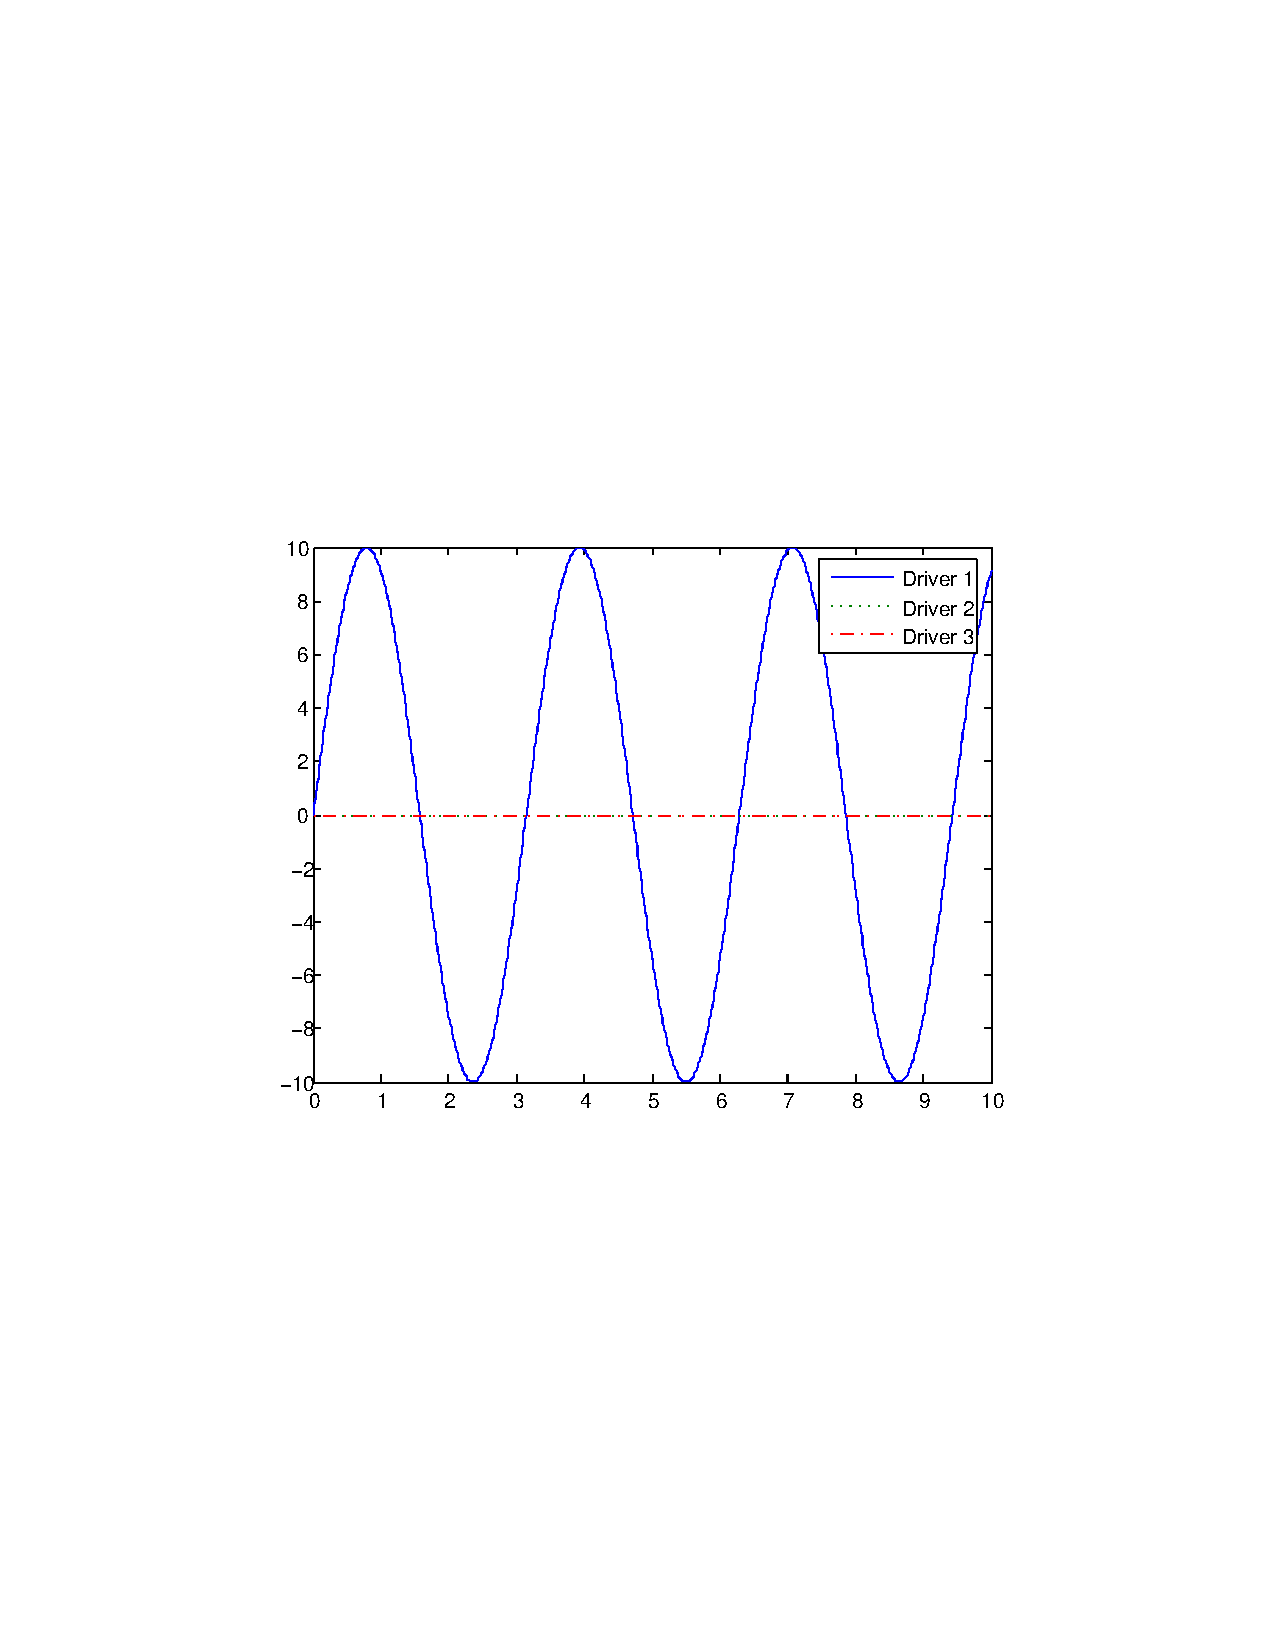
\includegraphics[width=\textwidth]{traffic_flow/traffic_flow_3cars_ODE_l0}
\end{center}
$\lambda=0$
}
\frame{
\begin{center}
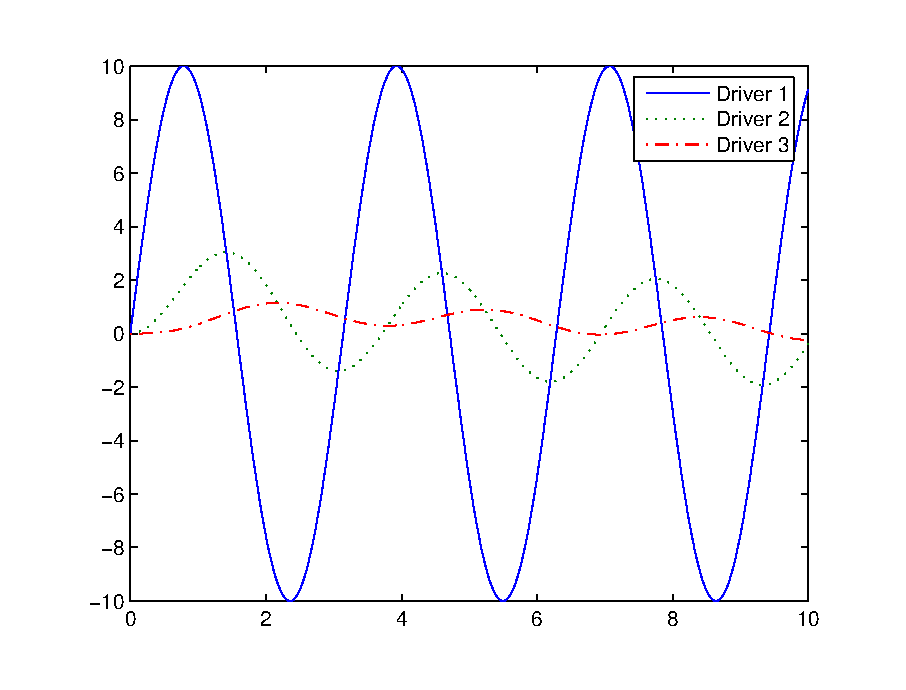
\includegraphics[width=\textwidth]{traffic_flow/traffic_flow_3cars_ODE_l04}
\end{center}
$\lambda=0.4$
}
\frame{
\begin{center}
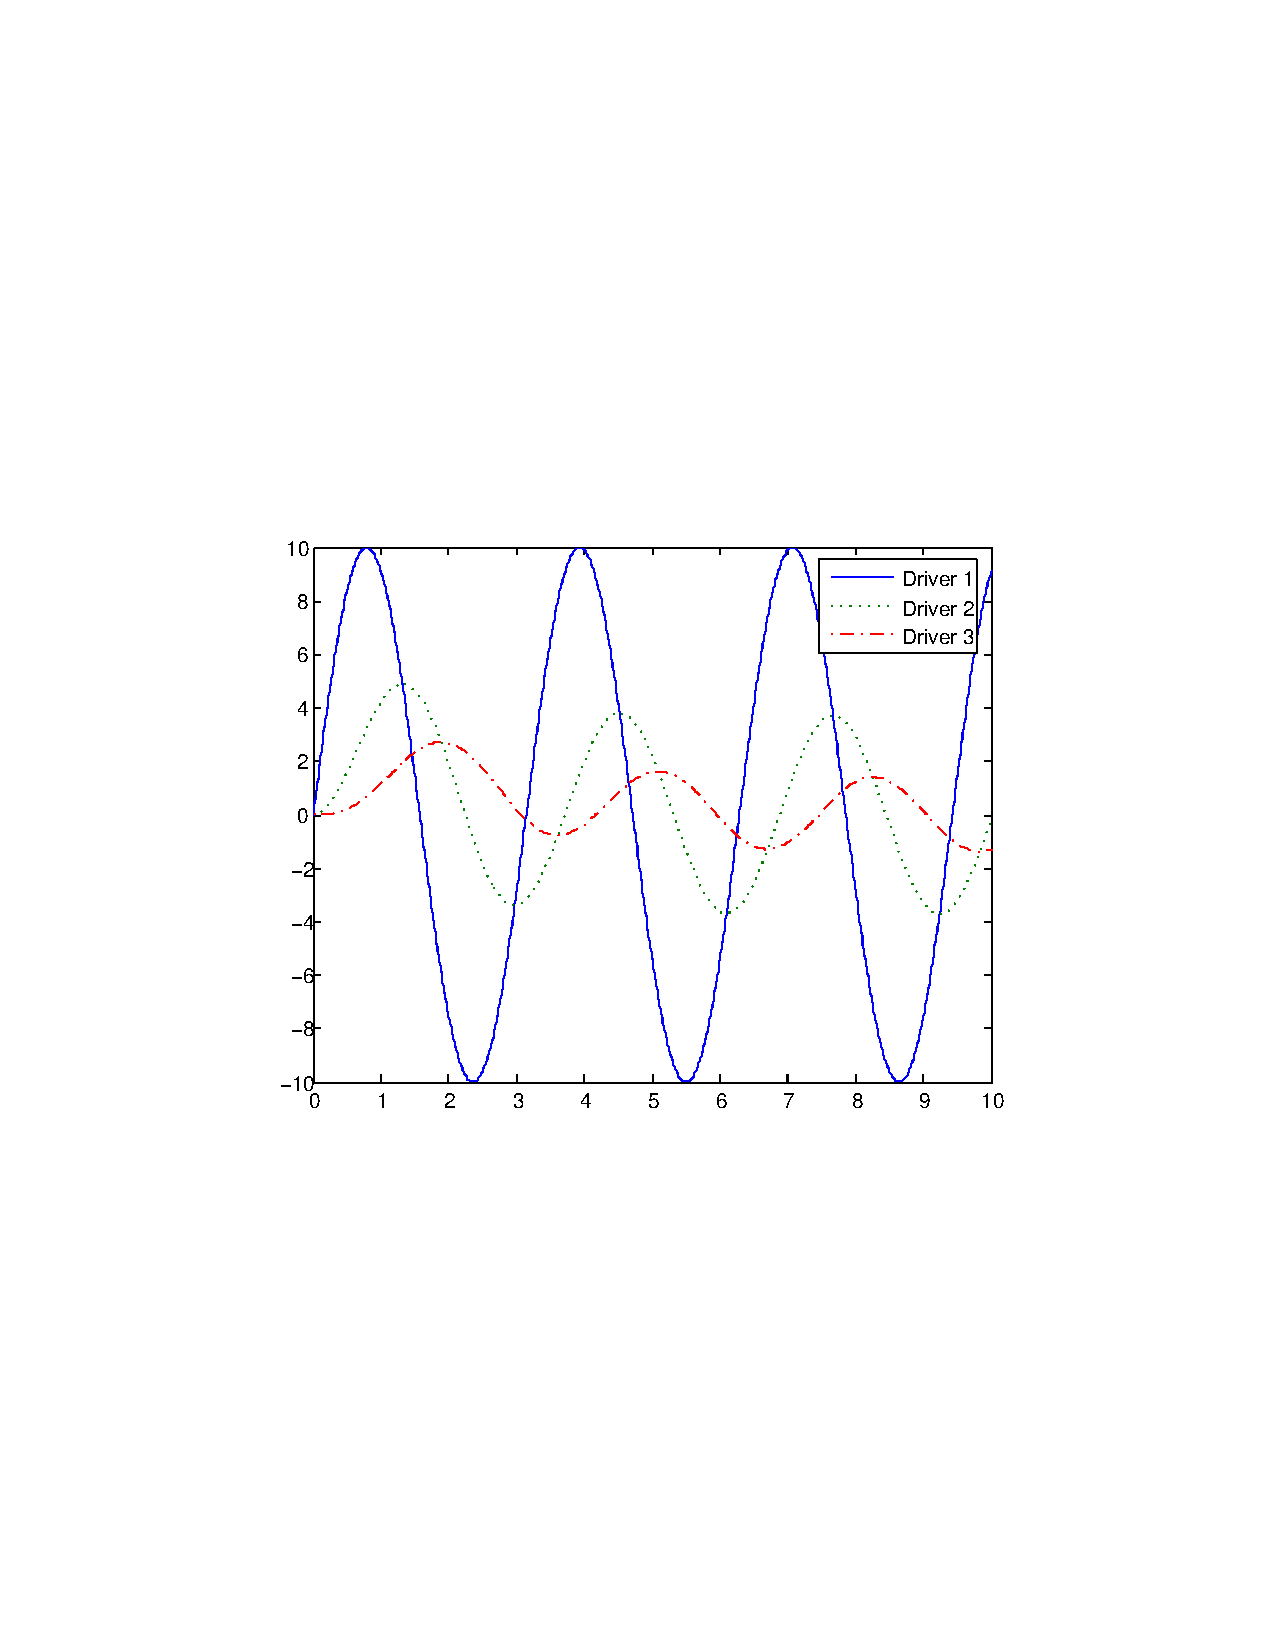
\includegraphics[width=\textwidth]{traffic_flow/traffic_flow_3cars_ODE_l08}
\end{center}
$\lambda=0.8$
}
\frame{
\begin{center}
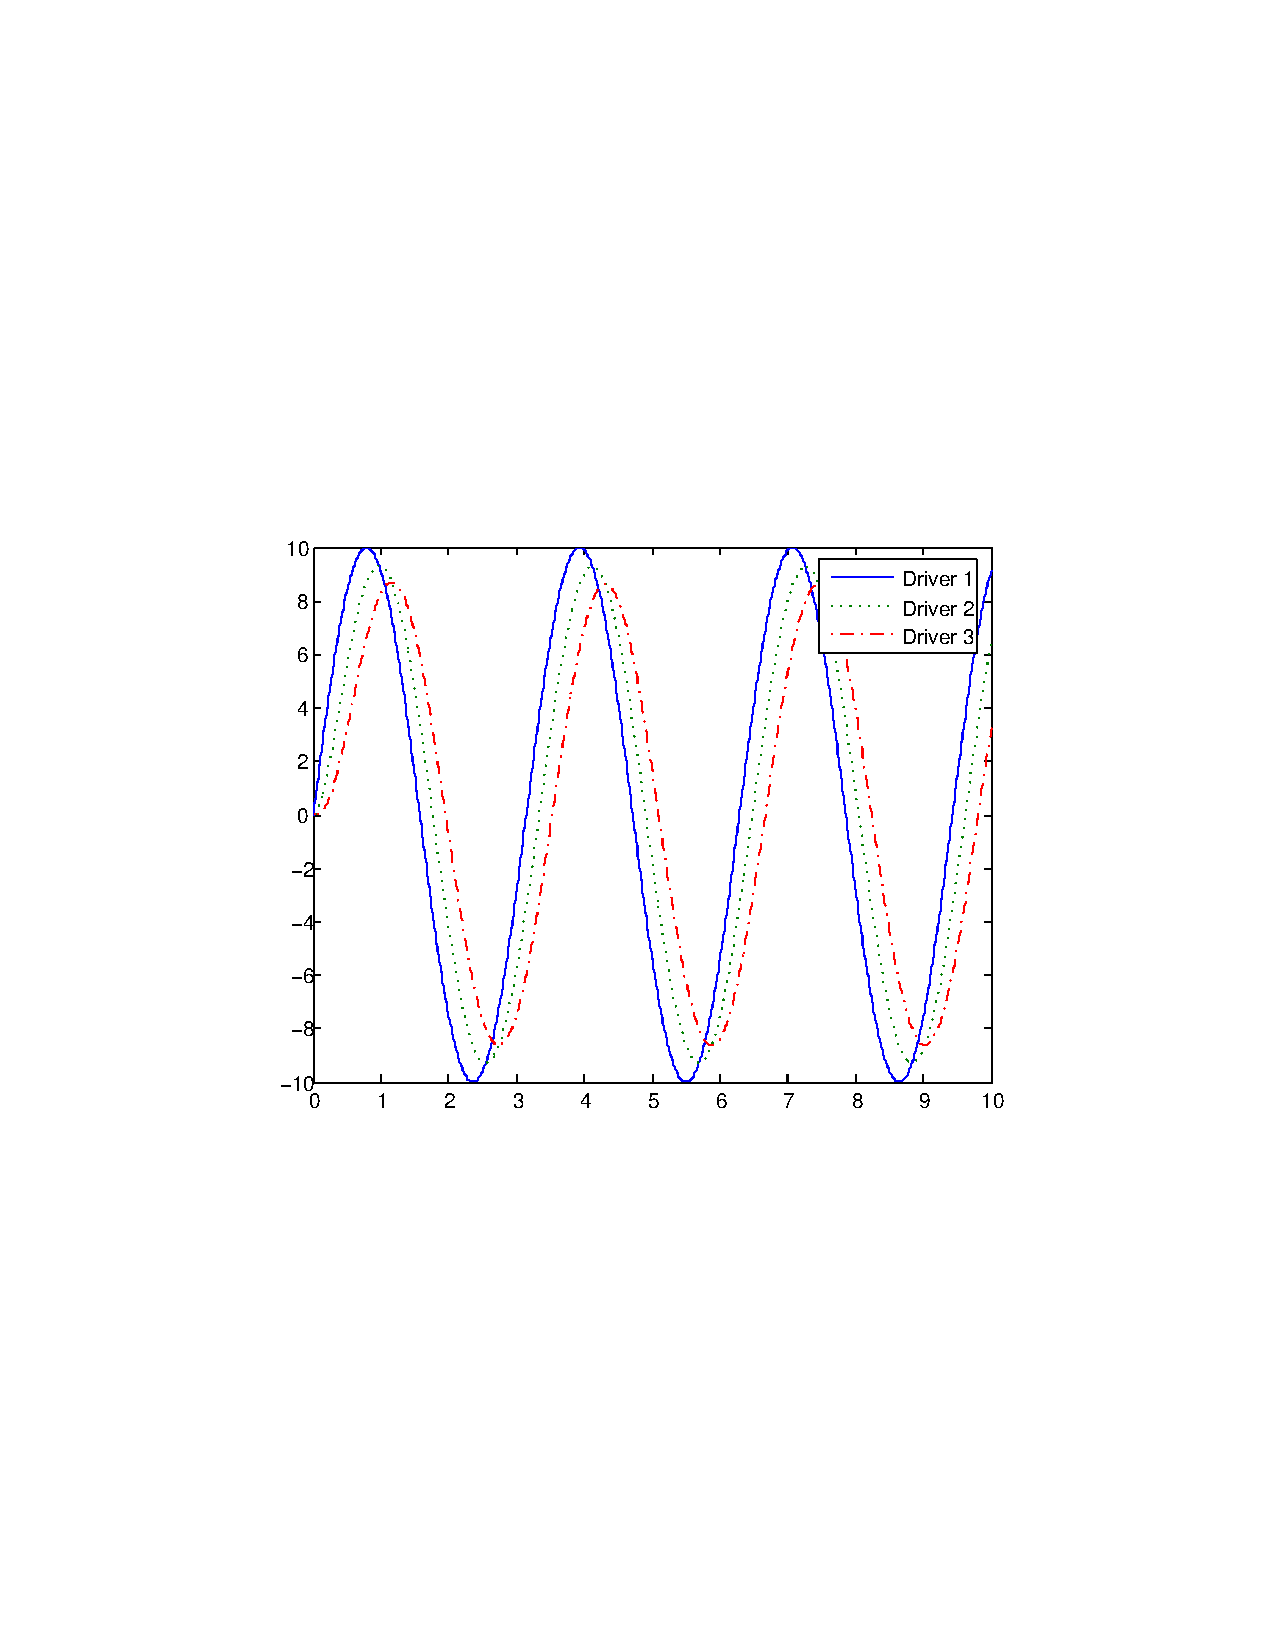
\includegraphics[width=\textwidth]{traffic_flow/traffic_flow_3cars_ODE_l5}
\end{center}
$\lambda=5$
}


\subsection{DDE model}

\frame{\frametitle{A delayed model of traffic flow}
We consider the same setting as previously, except that now, for $t>0$,
\begin{equation}\label{eq:dde}
u'_{n+1}(t)=\lambda(u_n(t-\tau)-u_{n+1}(t-\tau)),
\end{equation}
for $n=1,\ldots,N-1$. Here, $\tau\geq 0$ is called the \emph{time delay} (or \emph{time lag}), or for short, \emph{delay} (or \emph{lag}).

\vskip1cm
If $\tau=0$, we are back to the previous model.
}

\frame{\frametitle{Initial data}
For a delay equation such as \eqref{eq:dde}, the initial conditions become \emph{initial data}. This initial data must be specified on an interval of length $\tau$, left of zero.
\vskip0.5cm
This is easy to see by looking at the terms: $u(t-\tau)$ involves, at time $t$, the state of $u$ at time $t-\tau$. So if $t<\tau$, we need to know what happened for $t\in[-\tau,0]$.
\vskip0.5cm
So, normally, we specify initial data as
\[
u_n(t)=\phi(t)\textrm{ for }t\in[-\tau,0],
\]
where $\phi$ is some function, that we assume to be continuous. We assume $u_1(t)$ is known.
\vskip0.5cm
Here, we assume, for $n=1,\ldots,N$,
\[
u_n(t)=0,\qquad t\leq (n-1)\tau
\]
}

\frame{\frametitle{Important remark}
Although \eqref{eq:dde} looks very similar to \eqref{eq:ode}, you must keep in mind that it is in fact much more complicated.
\begin{itemize}
\item
A solution to \eqref{eq:ode} is a continuous function from $\IR$ to $\IR$ (or to $\IR^n$ if we consider the system).
\item
A solution to \eqref{eq:dde} is a continuous function in the space of continuous functions.
\item
The space $\IR^n$ has dimension $n$. The space of continuous functions has dimension $\infty$.
\end{itemize}
We then computed the Laplace transform of the system, but this was not very helpful, since, after solving the problem in $s$-space, we were not able to transform back into the original $t$-space.
}


%%%%%%%%%%%%%%
%%%%%%%%%%%%%%
%%%%%%%%%%%%%%
%%%%%%%%%%%%%%
\section{Shallow water waves}

\frame{\frametitle{Spatial domain}
We consider the motion of a body of water that is infinite in the $z$ direction, with or without boundary in the $x$ direction, and the vertical direction of gravity taken as the $y$ direction.
\begin{center}
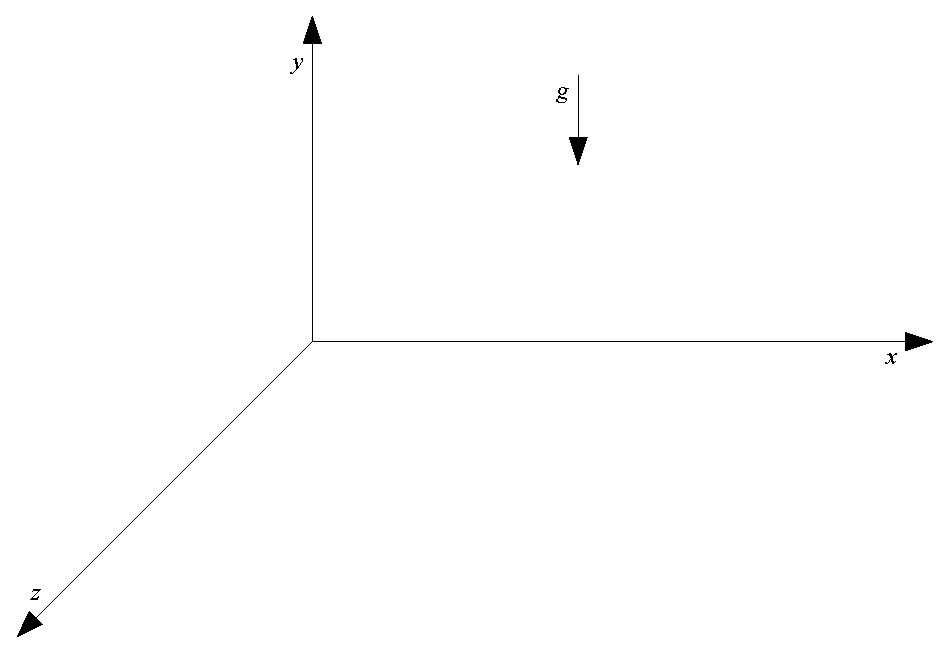
\includegraphics[width=0.7\textwidth]{shallow_water/xyz_domain}
\end{center}
From now on, suppose $z$ direction uniform (the same for all $z$), so ignore $z$ except for the sake of argument.
}



\frame{\frametitle{The one-dimensional wave equation (1)}
Following a long and complex argument, the following was derived.
\vskip1cm
The partial differential equation
\begin{equation}\label{eq:wave_zeta}
\zeta_{tt}=c^2\zeta_{xx}
\end{equation}
with $c^2=Hg$, is the one-dimensional wave equation. Initial conditions are given by
\begin{align*}
\zeta(x,0) &= h_0(x)-H\equiv\zeta_0(x) \\
\zeta_t(x,0) &= -Hu_x(x,0)=-H[u_0(x)]_x\equiv \nu_0(x)
\end{align*}
}

\frame{\frametitle{The one-dimensional wave equation (2)}
Things can also be expressed in terms of $u$. Using the same type of simplification used before for $\zeta$, we get
\begin{equation}\label{eq:wave_u}
u_{tt}=c^2u_{xx}
\end{equation}
with $c^2=Hg$. Initial conditions are given by
\begin{align*}
u(x,0) &= u_0(x) \\
u_t(x,0) &= -g\zeta_x(x,0)=-g[h_0(x)]_x\equiv v_0(x)
\end{align*}
}

\subsection{Traveling wave solutions}


\frame{\frametitle{Traveling wave solutions}
This was obtained by d'Alembert. Consider
\begin{equation}
u_{tt}=c^2u_{xx} \tag{\ref{eq:wave_u}}
\end{equation}
Note that this can be written as
\[
\left(\frac{\partial}{\partial t}-c\frac{\partial}{\partial x}\right)
\left(\frac{\partial}{\partial t}+c\frac{\partial}{\partial x}\right)u=0
\]
This implies that for any $F,G$, the sum
\[
u(x,t)=F(x-ct)+G(x+ct)
\]
satisfies \eqref{eq:wave_u}.
}

\frame{
Set
\[
u(x,0)=f(x)\qquad u_t(x,0)=g(x)
\]
Then d'Alembert's formula gives
\[
u(x,t) = \frac{f(x-ct) + f(x+ct)}{2} + \frac{1}{2c} \int_{x-ct}^{x+ct} g(s) ds
\]
}

\frame{\frametitle{Case of a Dirac delta initial condition}
Suppose $u_0(x)=0$ and $v_0(x)=\delta(x)$, for $-\infty<x<\infty$, with $\delta$ the Dirac delta,
\[
\delta(x)=\begin{cases}
\infty & \textrm{if }x=0\\
0 & \textrm{otherwise}.
\end{cases}
\]
Therefore,
\[
u(x,t)=\frac 1{2c}\int_{x-ct}^{x+ct}\delta(z)dz=\frac 1{2c}\left\{H(x+ct)-H(x-ct)\right\},
\]
with $H$ the Heaviside function,
\[
H(x)=\begin{cases}
0 & \textrm{if }x<0\\
1 & \textrm{if }x>0.
\end{cases}
\]
}

\frame{
For simplicity, take $c=1$. This gives
\[
u(x,t)=\frac 12\left\{H(x+t)-H(x-t)\right\},
\]
}

\frame{
\begin{center}
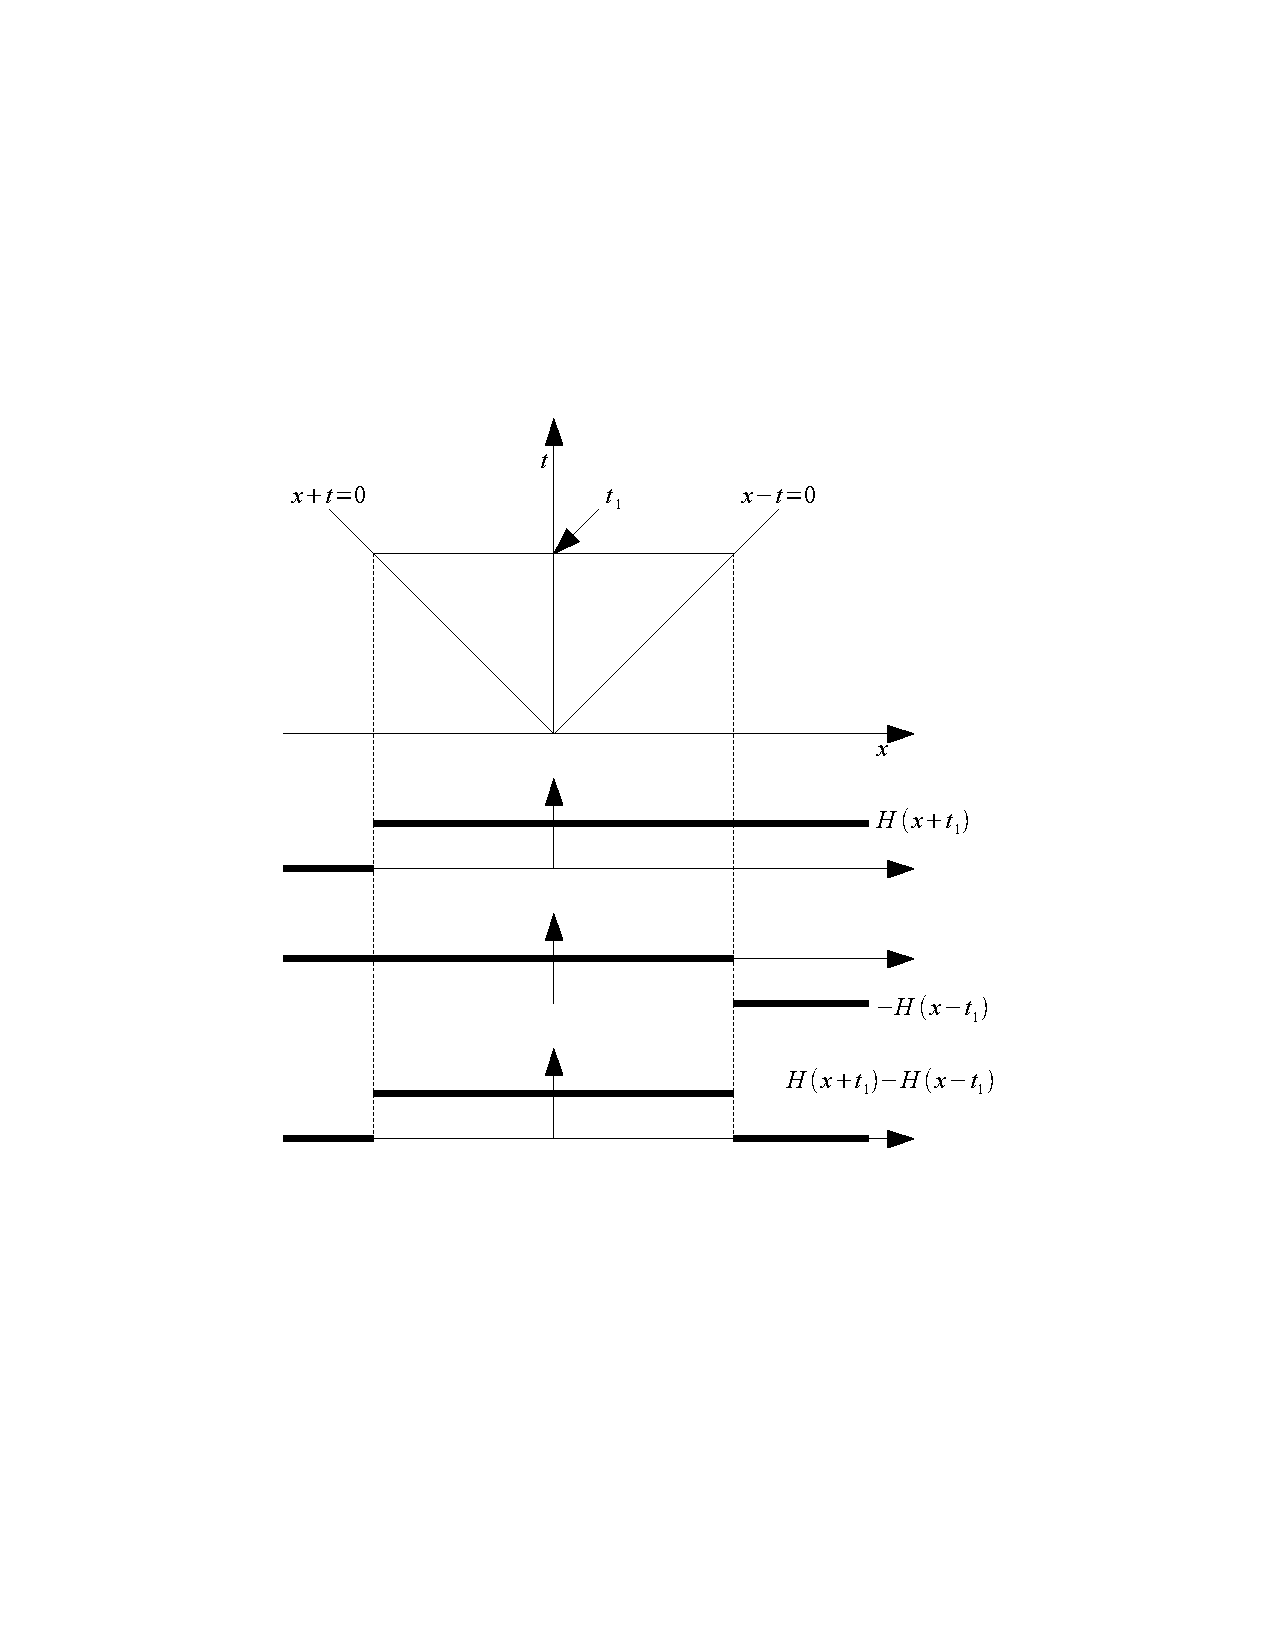
\includegraphics[height=0.95\textheight]{shallow_water/xct}
\end{center}
}

\frame{
As $t$ increases, we move further up in the top graph in $(x,t)$-space, resulting in a wider and wider square pulse.
\begin{center}
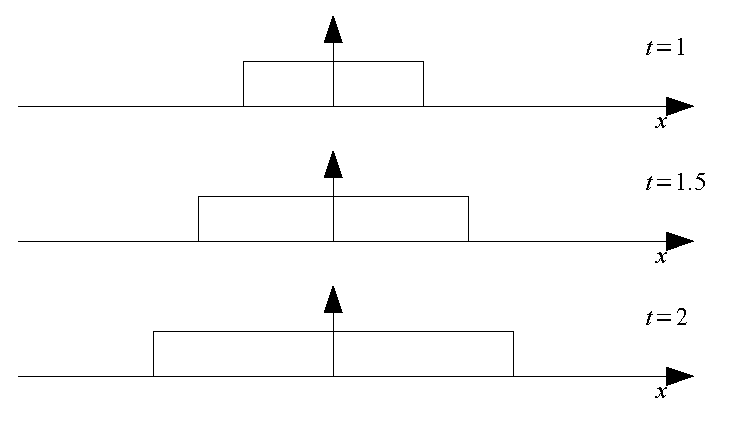
\includegraphics[width=\textwidth]{shallow_water/xwave}
\end{center}
}

%%%%%%%%%%%%%%
%%%%%%%%%%%%%%
%%%%%%%%%%%%%%
%%%%%%%%%%%%%%
\section{A simple genetic model}

\frame{\frametitle{Simple Mendelian inheritance}
A certain trait is determined by a specific pair of genes, each of which may be two types, say $G$ and $g$. 
\vskip0.4cm
One individual may have:
\begin{itemize}
\item $GG$ combination (\emph{dominant})
\item $Gg$ or $gG$, considered equivalent genetically (\emph{hybrid})
\item $gg$ combination (\emph{recessive})
\end{itemize}
\vskip0.4cm
In sexual reproduction, offspring inherit one gene of the pair from each parent. 
}

\frame{\frametitle{Basic assumption of Mendelian genetics}
Genes inherited from each parent are selected at random, independently of each other.
This determines probability
of occurrence of each type of offspring. The offspring
\begin{itemize}
\item of two $GG$ parents must be $GG$, 
\item of two $gg$ parents must be $gg$,
\item of one $GG$ and one $gg$ parent must be $Gg$,
\item other cases must be examined in more detail.
\end{itemize}
}

\frame{\frametitle{$GG$ and $Gg$ parents}
\begin{center}
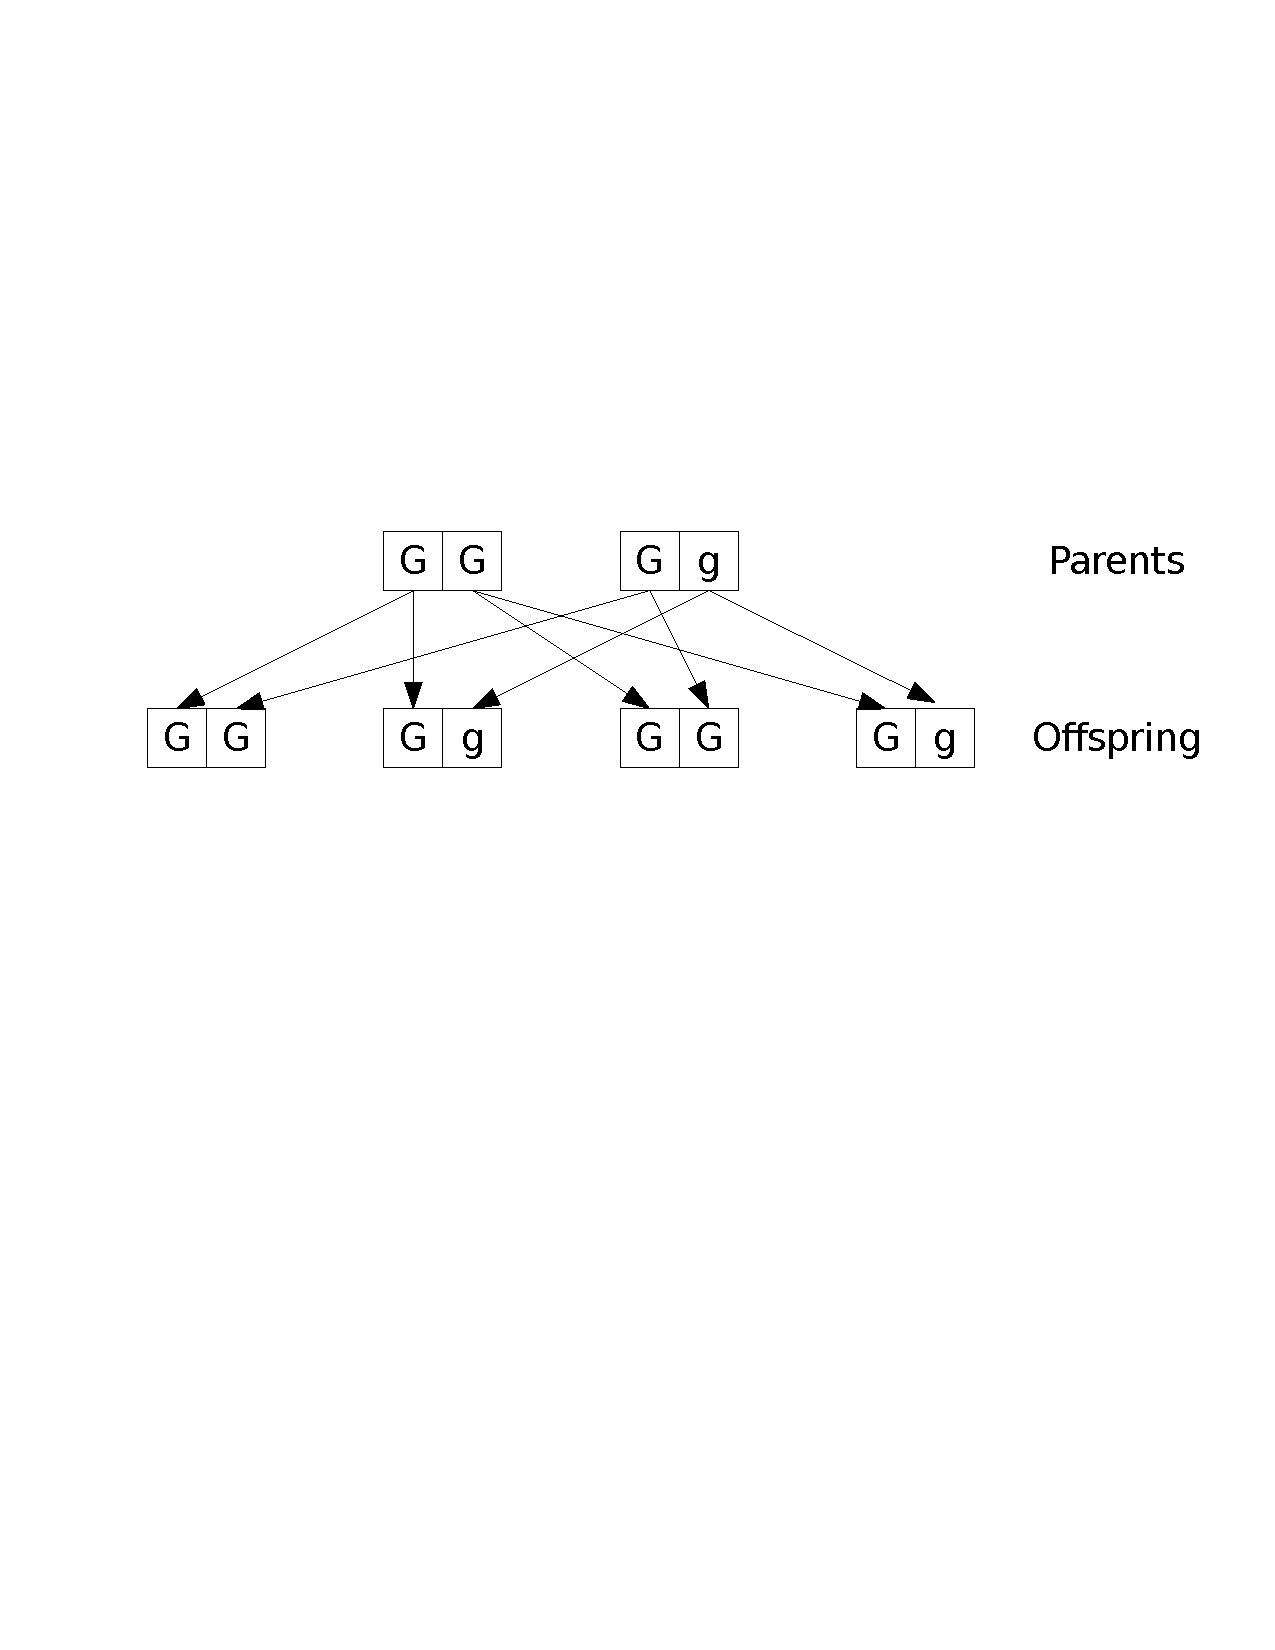
\includegraphics[width=0.9\textwidth]{genetics/dominant_hybrid}
\end{center}
\vskip0.3cm
Offspring has probability
\begin{itemize}
\item $\dfrac 12$ of being $GG$
\item $\dfrac 12$ of being $Gg$
\end{itemize}
}


\frame{\frametitle{$Gg$ and $Gg$ parents}
\begin{center}
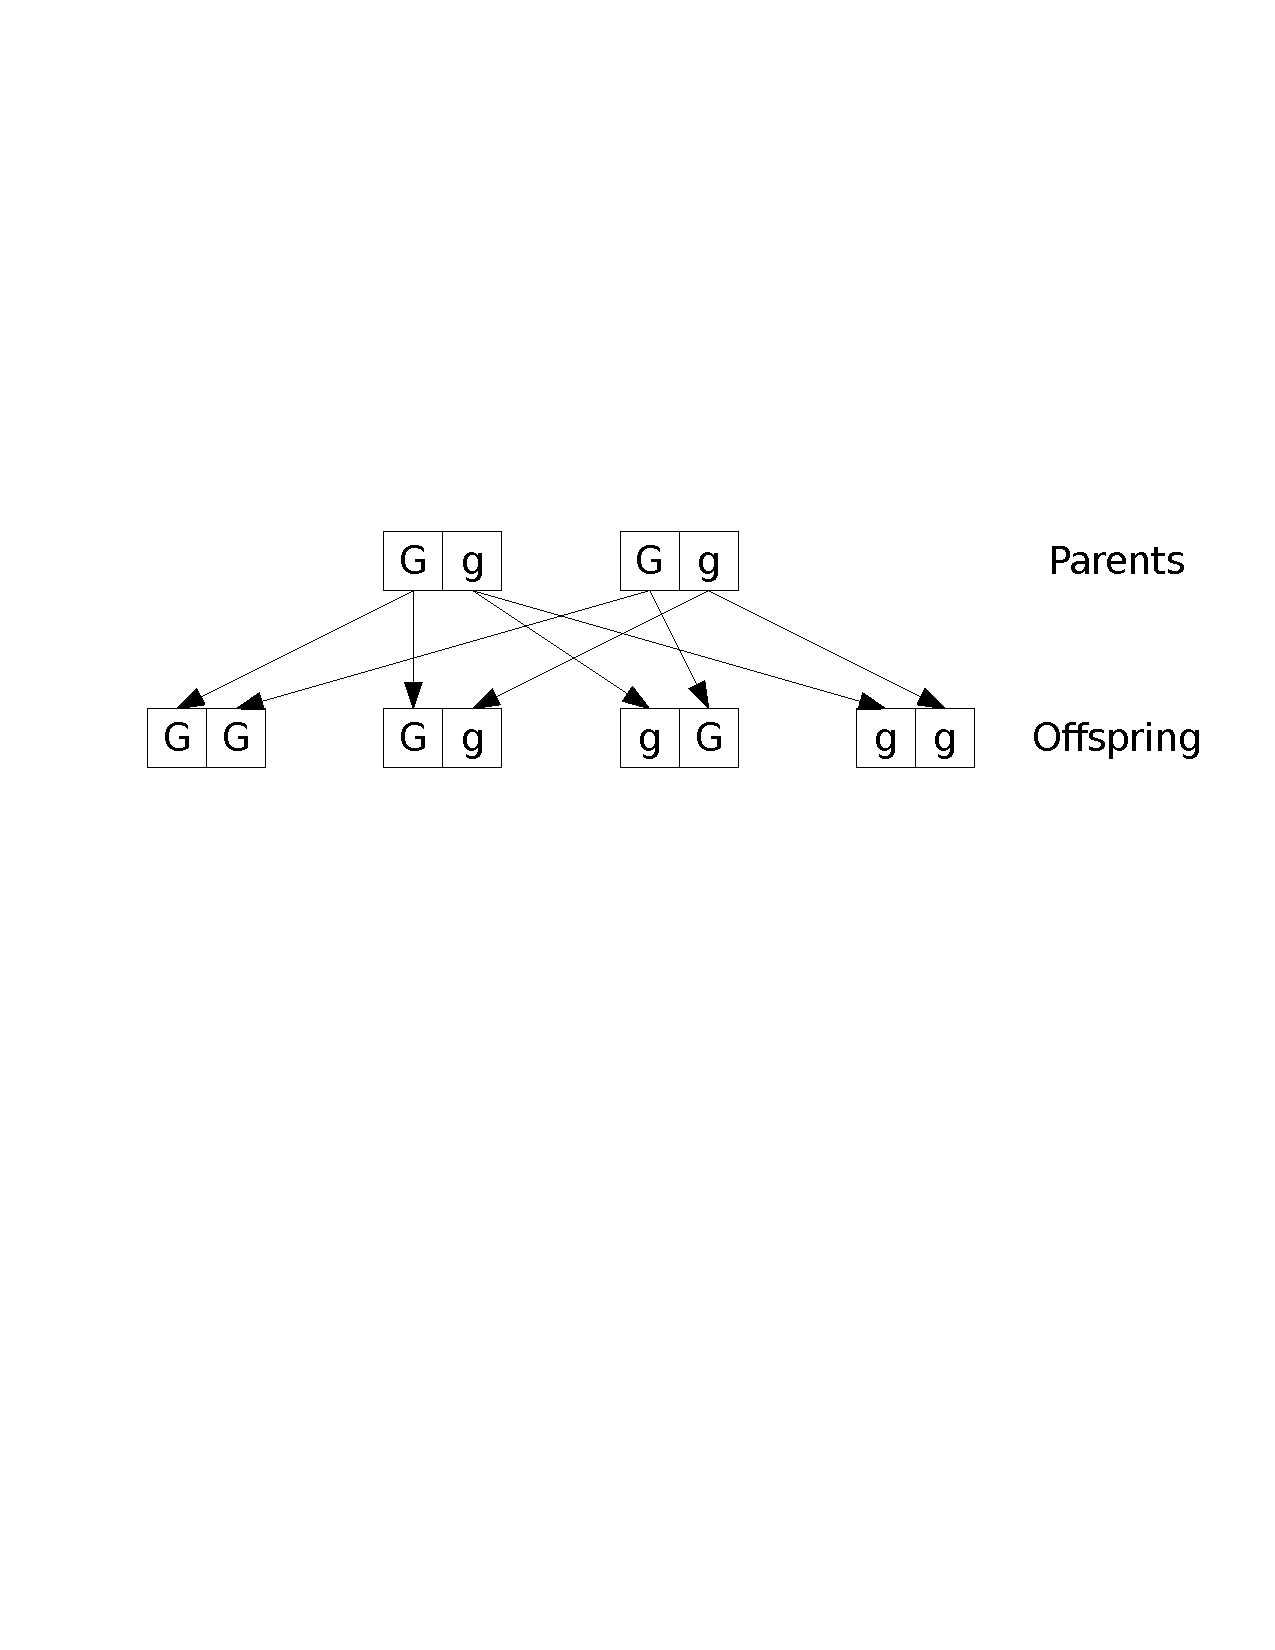
\includegraphics[width=0.9\textwidth]{genetics/hybrid_hybrid}
\end{center}
\vskip0.3cm
Offspring has probability
\begin{itemize}
\item $\dfrac 14$ of being $GG$
\item $\dfrac 12$ of being $Gg$
\item $\dfrac 14$ of being $gg$
\end{itemize}
}


\frame{\frametitle{$gg$ and $Gg$ parents}
\begin{center}
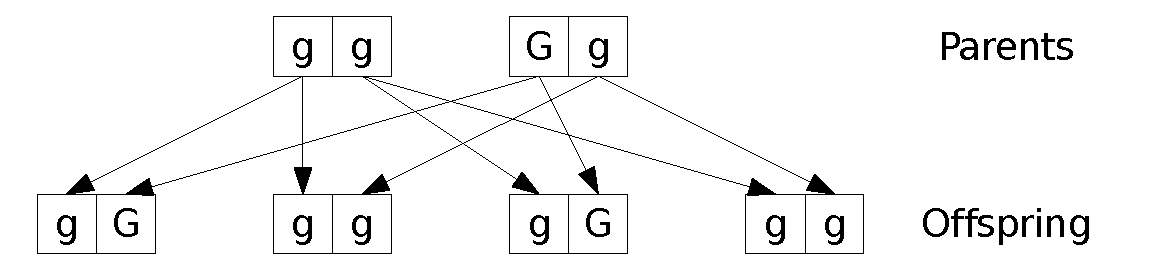
\includegraphics[width=0.9\textwidth]{genetics/recessive_hybrid}
\end{center}
\vskip0.3cm
Offspring has probability
\begin{itemize}
\item $\dfrac 12$ of being $Gg$
\item $\dfrac 12$ of being $gg$
\end{itemize}
}



\subsection{Continued matings with a $Gg$ individual -- Regular chain}

\frame{\frametitle{Continued matings}
Consider a process of continued matings. 
\begin{itemize}
\item Start with an individual of known or unknown
genetic character and mate it with a hybrid. 
\item Assume that there is at least one
offspring; choose one of them at random and mate it with a hybrid.
\item Repeat this process through a number of generations. 
\end{itemize}
The genetic type of the chosen
offspring in successive generations can be represented by a Markov chain, with states $GG$, $Gg$ and $gg$. So there are 3 possibles states $S_1=GG$, $S_2=Gg$ and $S_3=gg$.
}

\frame{
We have
\begin{center}
\begin{tabular}{c|ccc}
$\nearrow$ & GG & Gg & gg \\
\hline
GG & 0.5 & 0.5 & 0 \\
Gg & 0.25 & 0.5 & 0.25 \\
gg & 0 & 0.5 & 0.5
\end{tabular}
\end{center}
The transition probabilities are thus
\[
P=\left (
\begin{array}{ccc}
\frac 12 & \frac 12 & 0 \\
\frac 14 & \frac 12 & \frac 14 \\
0 & \frac 12 & \frac 12
\end{array}\right)
\]
}

\frame{
The Markov chain is here regular. Indeed, take the matrix $P$,
\[
P=\left (
\begin{array}{ccc}
\frac 12 & \frac 12 & 0 \\
\frac 14 & \frac 12 & \frac 14 \\
0 & \frac 12 & \frac 12
\end{array}\right)
\]
and compute $P^2$:
\[
P^2=\left (
\begin{array}{ccc}
\frac 38 & \frac 12 & \frac 18 \\
\frac 14 & \frac 12 & \frac 14 \\
\frac 18 & \frac 12 & \frac 38
\end{array}\right)
\]
As all entries are positive, $P$ is primitive and the Markov chain is regular.
}

\frame{
Another way to check regularity:
\begin{theorem}
A matrix $M$ is primitive if the associated connection graph is strongly connected, i.e., that there is a path between any pair $(i,j)$ of states, and that there is at least one positive entry on the diagonal of $M$.
\end{theorem}
This is checked directly on the transition graph
\begin{center}
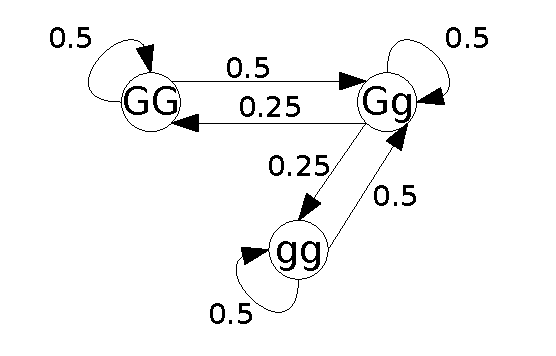
\includegraphics[width=0.6\textwidth]{genetics/graphe_hybride}
\end{center}
}

\frame{
Compute the left eigenvector associated to 1 by solving
\[
(w_1,w_2,w_3)
\left (
\begin{array}{ccc}
\frac 12 & \frac 12 & 0 \\
\frac 14 & \frac 12 & \frac 14 \\
0 & \frac 12 & \frac 12
\end{array}\right)=(w_1,w_2,w_3)
\]
\begin{subequations}
\begin{align}
\frac 12 w_1+\frac 14 w_2 &= w_1 \label{eq:l1} \\
\frac 12 w_1+\frac 12 w_2+\frac 12 w_3 &= w_2 \label{eq:l2} \\
\frac 14 w_2+\frac 12 w_3 &= w_3 \label{eq:l3} 
\end{align}
\end{subequations}
From \eqref{eq:l1}, $w_1=w_2/2$, and from \eqref{eq:l3}, $w_3=w_2/2$. Substituting these values into \eqref{eq:l2},
\[
\frac 14 w_2+\frac 12 w_2 +\frac 14 w_2=w_2,
\]
that is, $w_2=w_2$, i.e., $w_2$ can take any value. So $w=(\frac 14,\frac 12,\frac 14)$.
}

\subsection{Continued matings with a $GG$ individual -- Absorbing chain}


\frame{\frametitle{Mating with a $GG$ individual}
Suppose now that we conduct the same experiment, but mate each new generation with a $GG$ individual instead of a $Gg$ individual. Transition table is
\begin{center}
\begin{tabular}{c|ccc}
$\nearrow$ & GG & Gg & gg \\
\hline
GG & 1 & 0 & 0 \\
Gg & 0.5 & 0.5 & 0 \\
gg & 0 & 1 & 0
\end{tabular}
\end{center}
The transition probabilities are thus
\[
P=\left (
\begin{array}{ccc}
1 & 0 & 0 \\
\frac 12 & \frac 12 & 0 \\
0 & 1 & 0
\end{array}\right)
\]
}

\frame{\frametitle{New transition graph}
\begin{center}
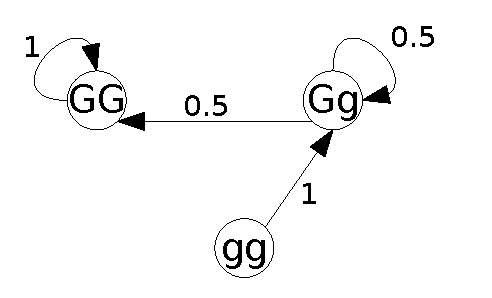
\includegraphics[width=0.8\textwidth]{genetics/graphe_dominant}
\end{center}
Clearly: 
\begin{itemize}
\item we leave $gg$ after one iteration, and can never return,
\item as soon as we leave $Gg$, we can never return,
\item can never leave $GG$ as soon as we get there.
\end{itemize}
}


\frame{
The matrix is already in standard form,
\[
P=\left (
\begin{array}{ccc}
1 & 0 & 0 \\
\frac 12 & \frac 12 & 0 \\
0 & 1 & 0
\end{array}\right)
=\begin{pmatrix}
\mathbb{I}_1 & \mathbf{0} \\
R & Q
\end{pmatrix}
\]
with $\mathbb{I}_1=1$, $\mathbf{0}=(0\;\; 0)$ and
\[
R=\begin{pmatrix}
\frac 12\\ 0
\end{pmatrix}
\qquad
Q=\begin{pmatrix}
\frac 12 & 0\\
1 & 0
\end{pmatrix}
\]
}

\frame{
We have
\[
\mathbb{I}_2-Q=\begin{pmatrix}
1 & 0 \\
0 & 1
\end{pmatrix}
-\begin{pmatrix}
\frac 12 & 0\\
1 & 0
\end{pmatrix}
=\begin{pmatrix}
\frac 12 & 0\\
-1 & 1
\end{pmatrix}
\]
so
\[
N=(\mathbb{I}_2-Q)^{-1}=
2\begin{pmatrix}
1 & 0 \\
1 & \frac 12
\end{pmatrix}=
\begin{pmatrix}
2 & 0 \\
2 & 1
\end{pmatrix}
\]
Then
\[
T=N\nbOne=\begin{pmatrix}
2\\
3
\end{pmatrix}
\]
and
\[
B=NR=
\begin{pmatrix}
2 & 0 \\
2 & 1
\end{pmatrix}
\begin{pmatrix}
\frac 12\\ 0
\end{pmatrix}
=
\begin{pmatrix}
1\\ 1
\end{pmatrix}
\]
}


\end{document}
